\chapter{Establishment of laboratory methods and analytical tools to assess genome-wide chromatin accessibility in clinical samples}
\chaptermark{Establishment of methods to assess genome-wide chromatin accessibility}
\label{ch:Results1}


%%%%%%%%%%%%%%%%%%%%%%%%%%%%%%%%%%%%%%%%%%%%%%%%%%
\section{Introduction}
\subsection*{Previous and current methods to identify the accessible genome in cells and tissues}

\subsection*{Implementation of ATAC-seq to define the chromatin landscape}

\subsection*{Technical limitations and recent advances in optimisation}
https://www.ncbi.nlm.nih.gov/pmc/articles/PMC4473780/

Talk about ATAC being more variable, a native chromatin accessibility assessment without cross-linking. Role of transposase ability in accessing the chromatin, debri and DNA from dead cells adding noise

ATAC-seq requires between 500 to 50,000 cells and is a fast two-steps protocol that yields information about open chromatin and nucleosome positioning simultaneously. 
These two aspects make ATAC-seq a very versatile technique to interrogate the chromatin landscape in a clinical set-up, where sample availability and time-efficiency are key factors \parencite{Scharer2016,Qu2015,Qu2017}. Regardless of the strengths of this new technique, ATAC-seq sensitivity is not comparable to DNase-seq for some cell types and tissues, and further optimisations of the first released protocol by Buenrostro and colleagues have been implemented \parencite{Corces2016,Sos2016,Corces2017}. 


Paper to justify peak calling: A comparison of peak callers used for DNase-Seq data.

New ATAC but also explanations of the limitations: Characterization of chromatin accessibility with a transposome hypersensitive sites sequencing (THS-seq) assay

\subsection*{Challenges of working with clinical samples}

%
\begin{landscape}
\begin{center}
\begin{longtable}[ht]{p{.20\textheight} p{.40\textheight} p{.40\textheight} p{.40\textheight}}
\caption[Summary table of ATAC-seq methodology analysis for peak calling, filtering and differential analysis.]{\textbf{.}}
\label{tab:ATAC_comparative_methods} \\
\toprule
\textbf{Publication} & \textbf{Peak calling and filtering} & \textbf{Master list} & \textbf{Differential analysis} \\
\midrule
\midrule
Corces \textit{et al.}, 2016 & MACS2 (-nomodel), peak summit extension $+/-$250bp, rank summits by pval & Maximally significant non-overlapping peaks. & Quantile normalisation and unsupervised hierarchical clustering. \\
&&&&
ENCODE  & MACS2 -nomodel, pairwise IDR analysis, filtering IDR$<$10\% & Choosing longest pairwise IDR filtered list or only peaks present in the two samples pseudoreplicates. & NA \\
&&&&              
Turner \textit{et al.}, 2018 	& MACS2 (-nomodel --q 0.01) & Merging all filtered called peaks from the different cell types. & \texti{De novo}:DiffReps with fragment size 50bp. \\                             
&&&&																																										
Alasoo \textit{et al.}, 2018 & MACS2 (-nomodel -shift -25 -extsize 50 --q 0.01 &	Union of peaks from all conditions present in at least in three samples of the same condition. & Peak based: TMM normalisation and lima voom (FDR$<$0.01).\\ 
&&&&
Qu \textit{et al.}, 2017 & ZINBA PP$>$0.99. & Merging of filtered peaks from each individual sample. & Quantile normalisation and peak based in house Pearson correlation method. \\							
&&&&
Rendeiro \textit{et al.} 2016 & MACS2 (-nomodel -extsize 147)	& Merge of peaks from all samples in an iterative process including permutations & Peak based: quantile normalisation and Fisher exact text (FDR$<$0.05). \\
&&&&
Scharer\textit{et al.} 2016 & HOMER (-style dnase) & Merge of all overlapping peaks between all samples using HOMER mergePeaks & Peak based: TMM normalisation and edgeR package (FDR$<$0.05). \\														   
\bottomrule
\medskip
\end{longtable}
\end{center}
\end{landscape}



%%%%%%%%%%%%%%%%%%%%%%%%%%%%%%%%%%%%%%%%%%%%%%%%%%
\section{Results}
%

\subsection{Establishment of an ATAC-seq data analysis pipeline based on current knowledge}
At the time of the first ATAC-seq publication \parencite{Buenrostro2013}, well established protocols for the complete processing and data analysis were missing. Since then, several publications have implemented ATAC-seq and modifications of this protocol together with a wide range of data analysis strategies to answer different biological questions (Table \ref{tab:ATAC_comparative_methods}).
In the process of analysing ATAC-seq data, several limiting aspects are encountered, including quality control (QC) assessment, peak calling/filtering and identification of differential chromatin accessibility regions between groups of samples. Using the current knowledge in the field as well as own analysis, the most appropriate criteria and parameters to implement in the in-house pipeline were agreed. For this purpose different types of analysis were performed using ATAC-seq data generated with the \parencite{Buenrostro2013} protocol in paired CD14$^+$ monocytes and total CD4$^+$ T cells from three healthy individuals. 


\subsubsection{Sample quality control}
%all of them downsamples to 30 million of reads, in order to facilitate the comparison across all of them.
Regarding QC measurements, the variability in performance of the methodology, particularly ATAC-seq and FAST-ATAC, has required identify appropriate parameters to determine the quality of the samples before proceeding with downstream differential analysis. This has been a dynamic process during the project that has benefited from the increase in the number of publications including ATAC-seq data analysis as well as identifying some of the limitations from the different protocols. After continuous review of the different read-outs implemented across different publications, as well as the recently ENCODE updates, a comprehensive analysis was performed in order to identify the most informative QC measures as well as equivalence and correlation between them.

The first analysed measure was the fragment size distribution for each of the six samples downsampled to 30 million of total reads after filtering (to facilitate the comparison across them). This measure allowed to determine recapitulation of nucleosome periodicity protecting the DNA during the transposition event (Figure \ref{fig:QC_ATAC}a), which is characteristic of ATAC-seq libraries. All the samples presented appropriate periodicity every $\sim$200bp up to 600bp, clearly distinguishing chromatin organisation into mono-, di- and tri-nucleosomes. The relative intensity of nucleosome-free DNA fragments ($<$$\sim$147pb) compared to nucleosome-bound DNA was greater for some of the samples (e.g CTL1 CD4$^+$ and CD14$^+$) and similar or lower for others (e.g CTL3 CD4$^+$ and CD14$^+$), which could be related to the overall library quality. %need to establish links with TSS or sth later
Nucleosome-free fragments(peak$<$$\sim$147bp) were also clearly distinguished in all of the samples and can be considered a compulsory requirement for ATAC-seq libraries passing QC according to the latest ENCODE recommendations \parencite{ENCODE}.


\begin{figure}[htbp]
\centering
\begin{subfigure}[b]{0.45\textwidth}
\centering
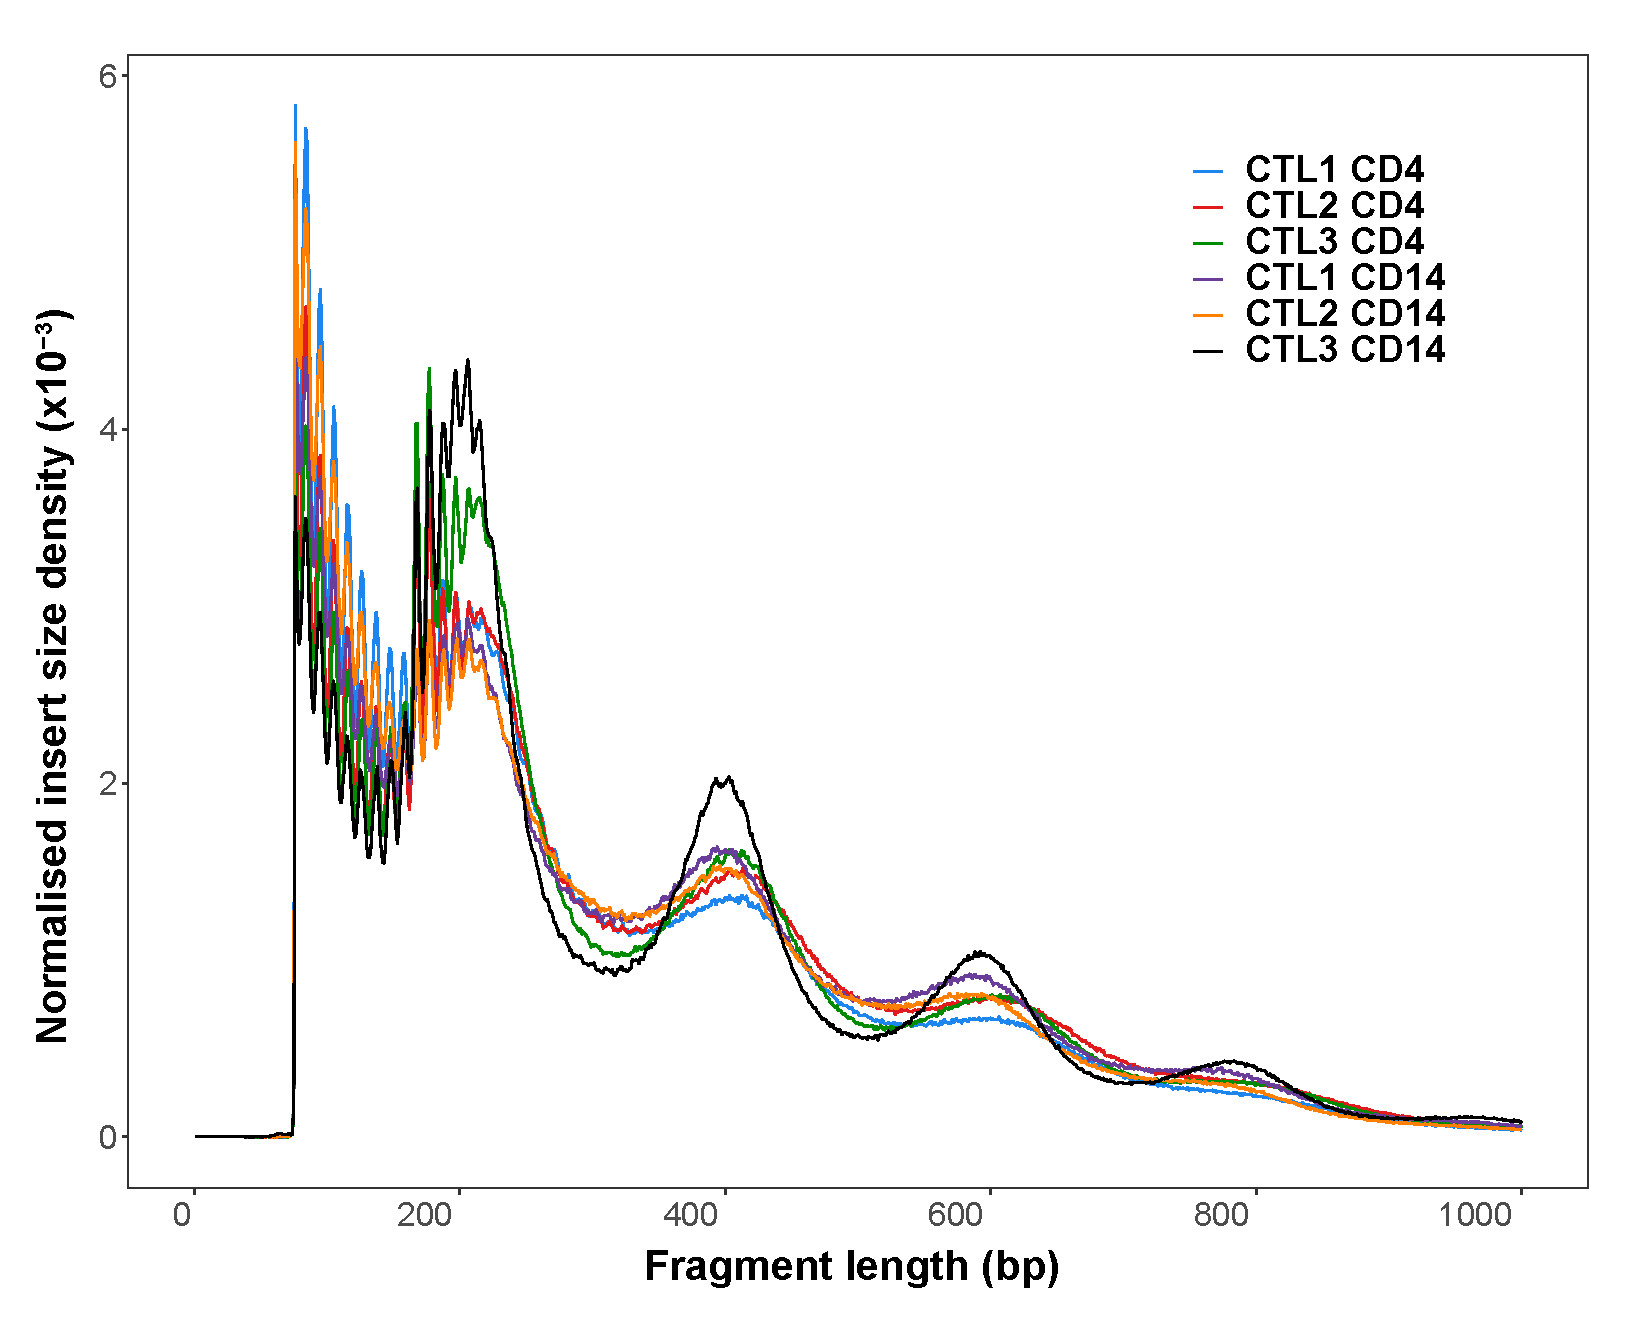
\includegraphics[width=\textwidth]{./Results1/pdfs/ATAC_Core_fresh_CD4_CD14_frag_size_distribution}
\caption{\textbf{}}
\end{subfigure}%
\begin{subfigure}[b]{0.45\textwidth}
\centering
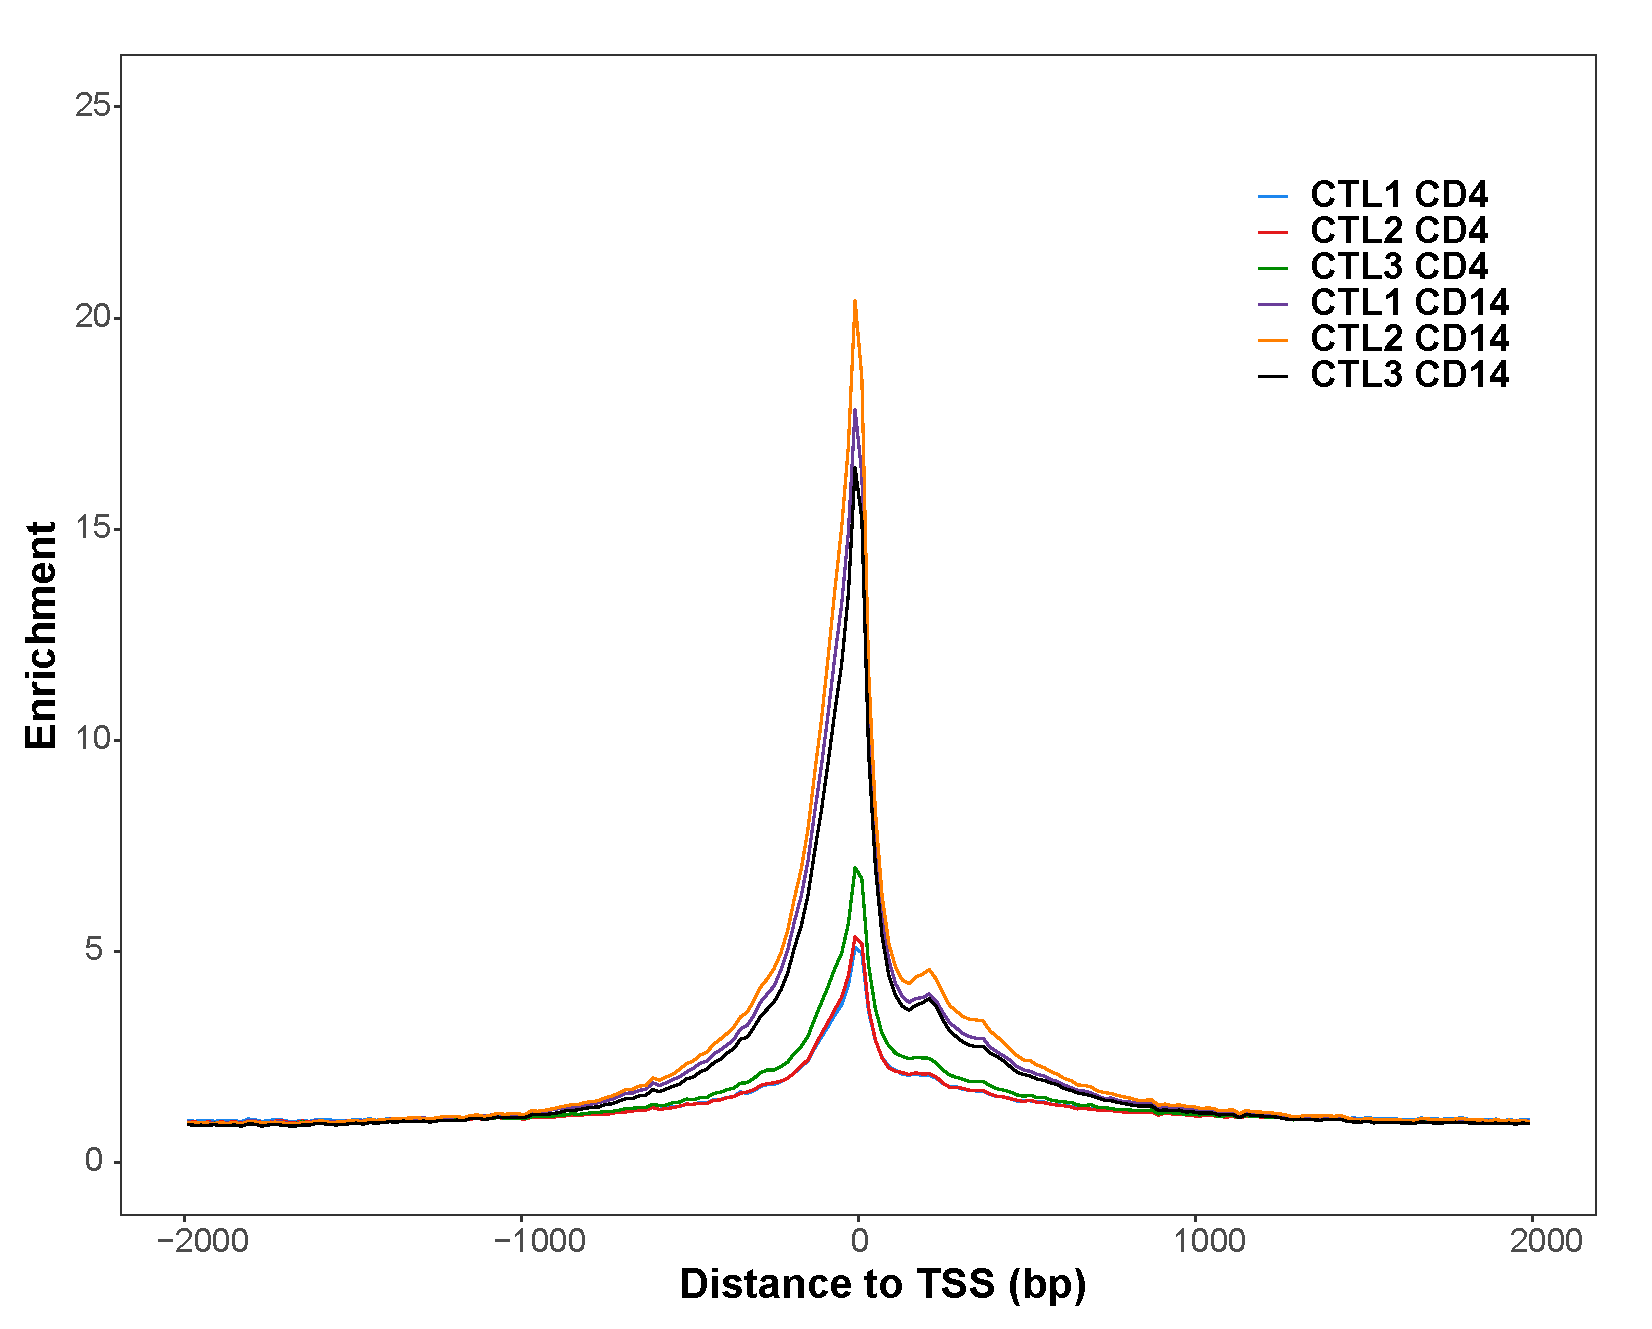
\includegraphics[width=\textwidth]{./Results1/pdfs/TSS_enrichment_Core_fresh_CD4_CD14}
\caption{\textbf{}}
\end{subfigure}
\begin{subfigure}[b]{0.6\textwidth}
\centering
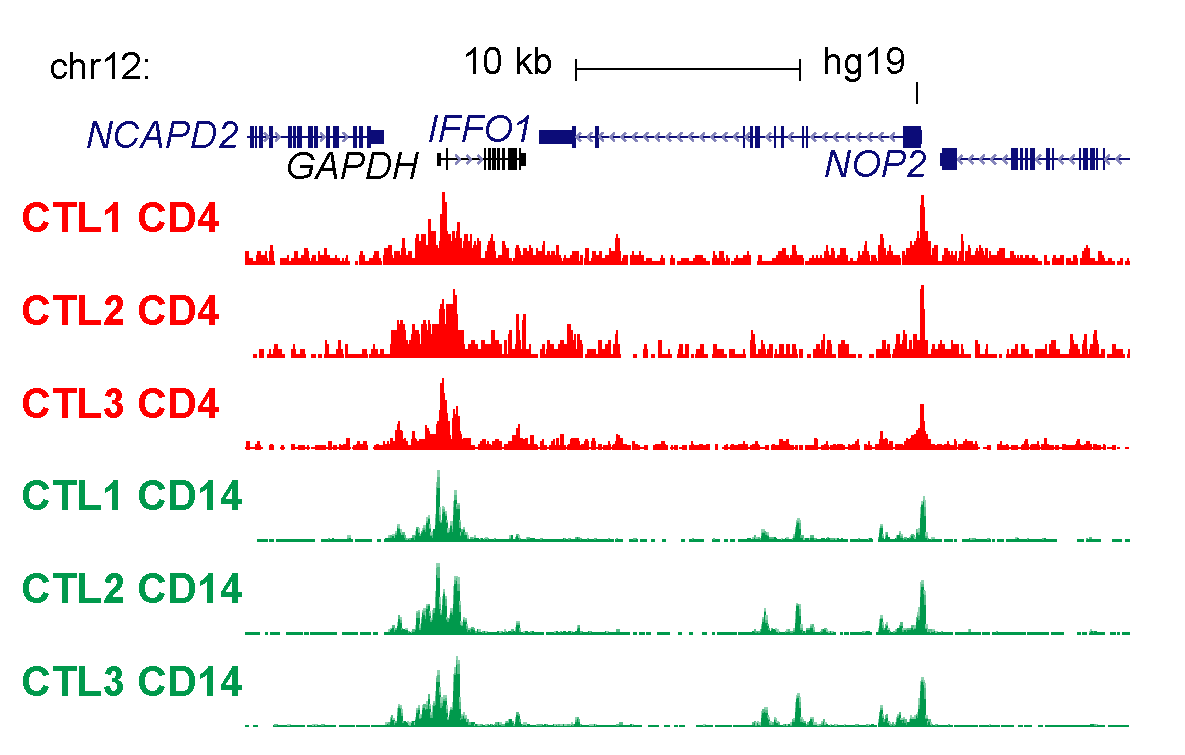
\includegraphics[width=\textwidth]{./Results1/pdfs/ATAC_Core_CD4_CD14_fresh_GAPDH}
\caption{\textbf{}} % to add text to the figure name
\end{subfigure}
\caption[Measurements for quality control assessment in ATAC-seq samples]{\textbf{Measurements for quality control assessment in ATAC-seq samples}}
\label{fig:QC_ATAC}
\end{figure} 



Another QC measurement that was investigated and implemented was the enrichment of ATAC-seq signal over a random background of reads across all the TSS identified for Ensemble genes (Figure \ref{fig:QC_ATAC}b). It is well established that nucleosome repositioning and an increase in chromatin accessibility take place at the genes TSS to allow TFs binding and initiation of transcription. Fold-enrichment signals over the TSS ranged between 5-7 for the CD4$^+$ samples being much higher(between 17-20) in the CD14$^+$ samples. The lower sample quality of the CD4$^+$ compared to CD14$^+$ samples indicated by the TSS enrichment values were recapitulated by the ATAC-seq reads pile up at the promoters of the glyceraldehyde-3-phosphate dehydrogenase (\textit{GAPDH}) and the NOP2 Nucleolar Protein gene \textit{NOP2} , presenting more background reads and less define signal for the CD4$^+$ samples in red (Figure \ref{fig:QC_ATAC}c).
	
As part of the QC assessment, the percentage of mitochondrial reads and the fraction of reads in peaks (FRiP) were also investigated (Table \ref{tab:ATAC_MT_fraction_reads_in_peaks}). 

\begin{table}[htbp]
%\setlength{\tabcolsep}{20pt} only to stretch the columns if you want
%\renewcommand{\arraystretch}{1.5}
\centering
\begin{tabular}{@{} c c c}
\toprule
\textbf{Sample} & \textbf{\% MT reads} & \textbf{Fraction of reads in peaks} \\
\midrule
\midrule
CTL1 CD4 & 14.9 & 9.8 \\
CTL2 CD4 & 30.5 & 11.2 \\
CTL3 CD4 & 28.8 & 11.6 \\
CTL1 CD14 & 43.3 & 32.2 \\
CTL2 CD14 & 36.8 & 57.0 \\
CTL3 CD14 & 37.6 & 49.9 \\
\bottomrule
\end{tabular}
\medskip %gap
\caption[ATAC-seq percentage of MT reads and fraction of reads in called peaks]{\textbf{}}
\label{tab:ATAC_MT_fraction_reads_in_peaks}
\end{table}
\bigskip %bigger space


FRiP score is an alternative way to TSS of assessing the background signal in different types of assays that are based on peak calling, including ChIP-seq. Positive correlation between the TSS fold-change enrichment and FRiP was observed (data not shown), being both appropriate inter-dependent QC measures to evaluate sample noise.  The mitochondrial content ranged between 14.9-43.3\% and, alike FRiP and TSS, it was higher in CD14$^+$ than in CD4$^+$ and not directly related with any of the other QC measurements. Therefore, MT reads in this range did not appear to reflect in the samples quality and the main inconvenience related to the need of deeper sequencing to achieve the desired number of no MT reads for doenstream analysis.

In summary, both TSS and FRiP appeared as appropriate signal-to-noise measures with recommended cut-ff values by ENCODE and Alsoo \textit{et al.}, 2018 being a minimum FRiP between 10-20\% and TSS between 6-10. Importantly ENCODE has prioritised the use of TSS over FRiP as a more stable measure to determine the noise in the sample and will also be the chosen measure in this study. Overall, according to this analysis, all six samples passed library QC and TSS enrichment recapitulated successfully the noticeable the differences observed in the ATAC-seq signal of the UCSC tracks, between the CD4$^+$ and CD14$^+$ samples.
	

\subsubsection{Peak calling and filtering}
As part of the ATAC-seq pipeline implementation, peak calling and their their filtering criteria were another two aspects to determine.
Although different peak callers have been used to analyse ATAC-seq data, MACS2 has been the preferred methodology by ENCODE and most of the publications (Table \ref{tab:ATAC_comparative_methods}). MACS2 has initially been developed for ChIP data, but it has also been used for DHS and ATAC-seq disabling the model option and manually setting the shift (--shift) and extension size (--extsize), which refer to the number of bp and direction for the reads to be shifted and the number of bp for them to be extended, respectively. Since the --extsize should correspond to the average fragment size, it was set to 200bp which was the average fragment size calculated for the ATAC-seq libraries in this project. The --shift was set to -100, as it is recommended to be -1/2 of the fragment size when analysing chromatin accessibility data, such as DHS or ATAC-seq. 

Although the optimisation of the previous parameter escaped from the aim of this thesis, a systematic analysis of the effect of sequencing depth and the sample quality on the peak calling was conducted to better control the effect of both variables in the downstream analysis. For each of the six samples, random sub-sampling of reads was performed every 5 million, ranging from 5 to 30 total million reads, and followed by peak calling with arbitrary filtering for FDR$<$0.01. The number of called peaks passing filtering showed an steady increase over the read depth reaching a \textit{plateau} at approximately 25M reads (Figure \ref{fig:Peak_calling_versus_depth_ATAC}a). This was consistent with the decay in the increments of called peaks over read depth, almost invariable, from 20M reads onwards (Figure \ref{fig:Peak_calling_versus_depth_ATAC}b). Moreover, lower number of peaks were detected in CD4$^+$ samples compared to CD14$^+$ highlighting the influence of sample quality on the total number of called peaks. Interestingly, sample quality measured by FRiP reflected very low changes over read depth and was stable from 15M reads onwards for all six samples (Figure \ref{fig:Peak_calling_versus_depth_ATAC}c), similar.ly to TSS (data not shown). Overall, this confirmed that measurement of sample quality using FRiP or TSS was not affected by the sequencing depth.


\begin{figure}[htbp]
\centering
\begin{subfigure}{0.50\textwidth}
\centering
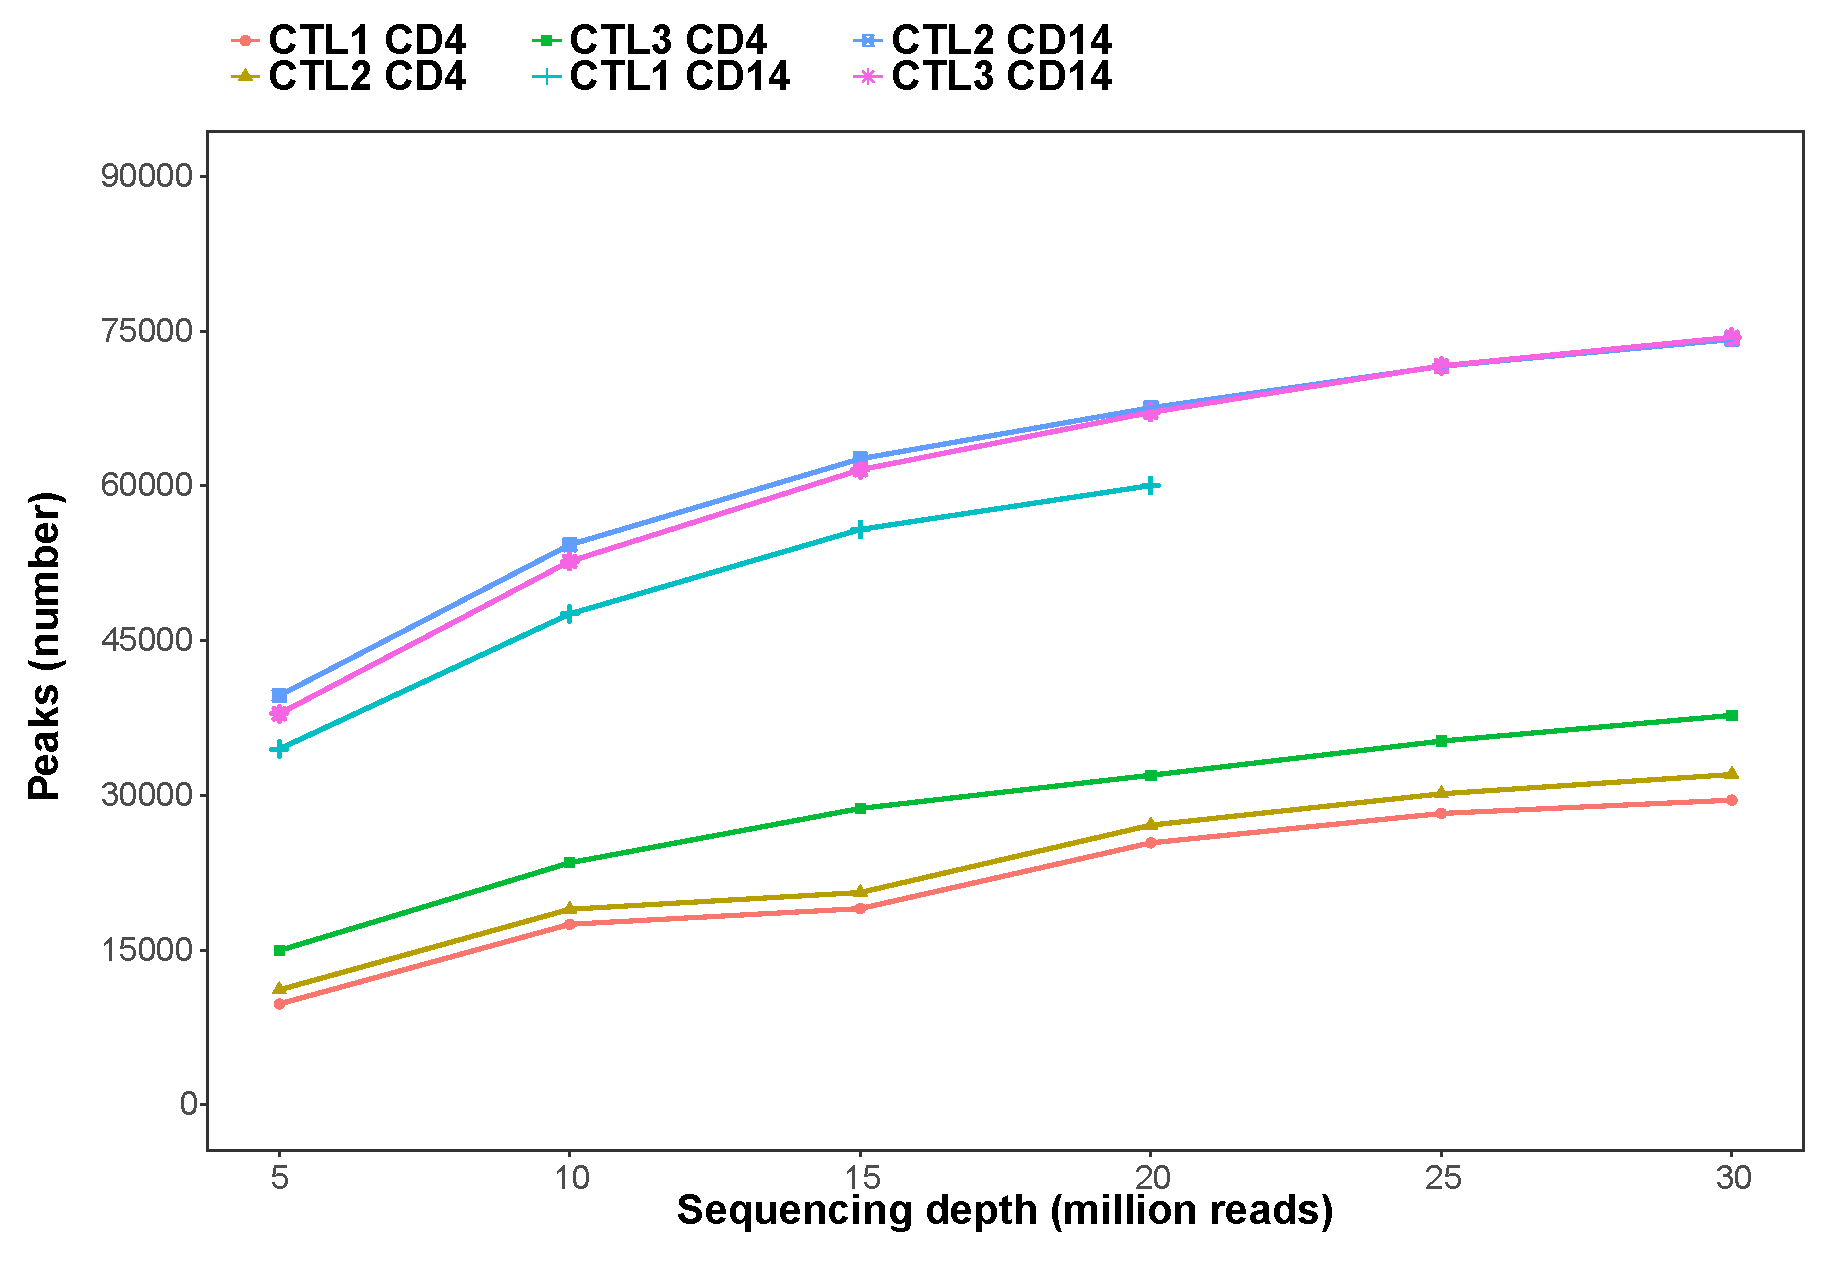
\includegraphics[width=\textwidth]{./Results1/pdfs/ATAC_Core_fresh_CD4_CD14_num_peaks_vs_depth}
\caption{\textbf{}}
% The percentage sign indicated that the other subfig goes side by side
\end{subfigure} \\
\begin{subfigure}{0.45\textwidth}
\centering
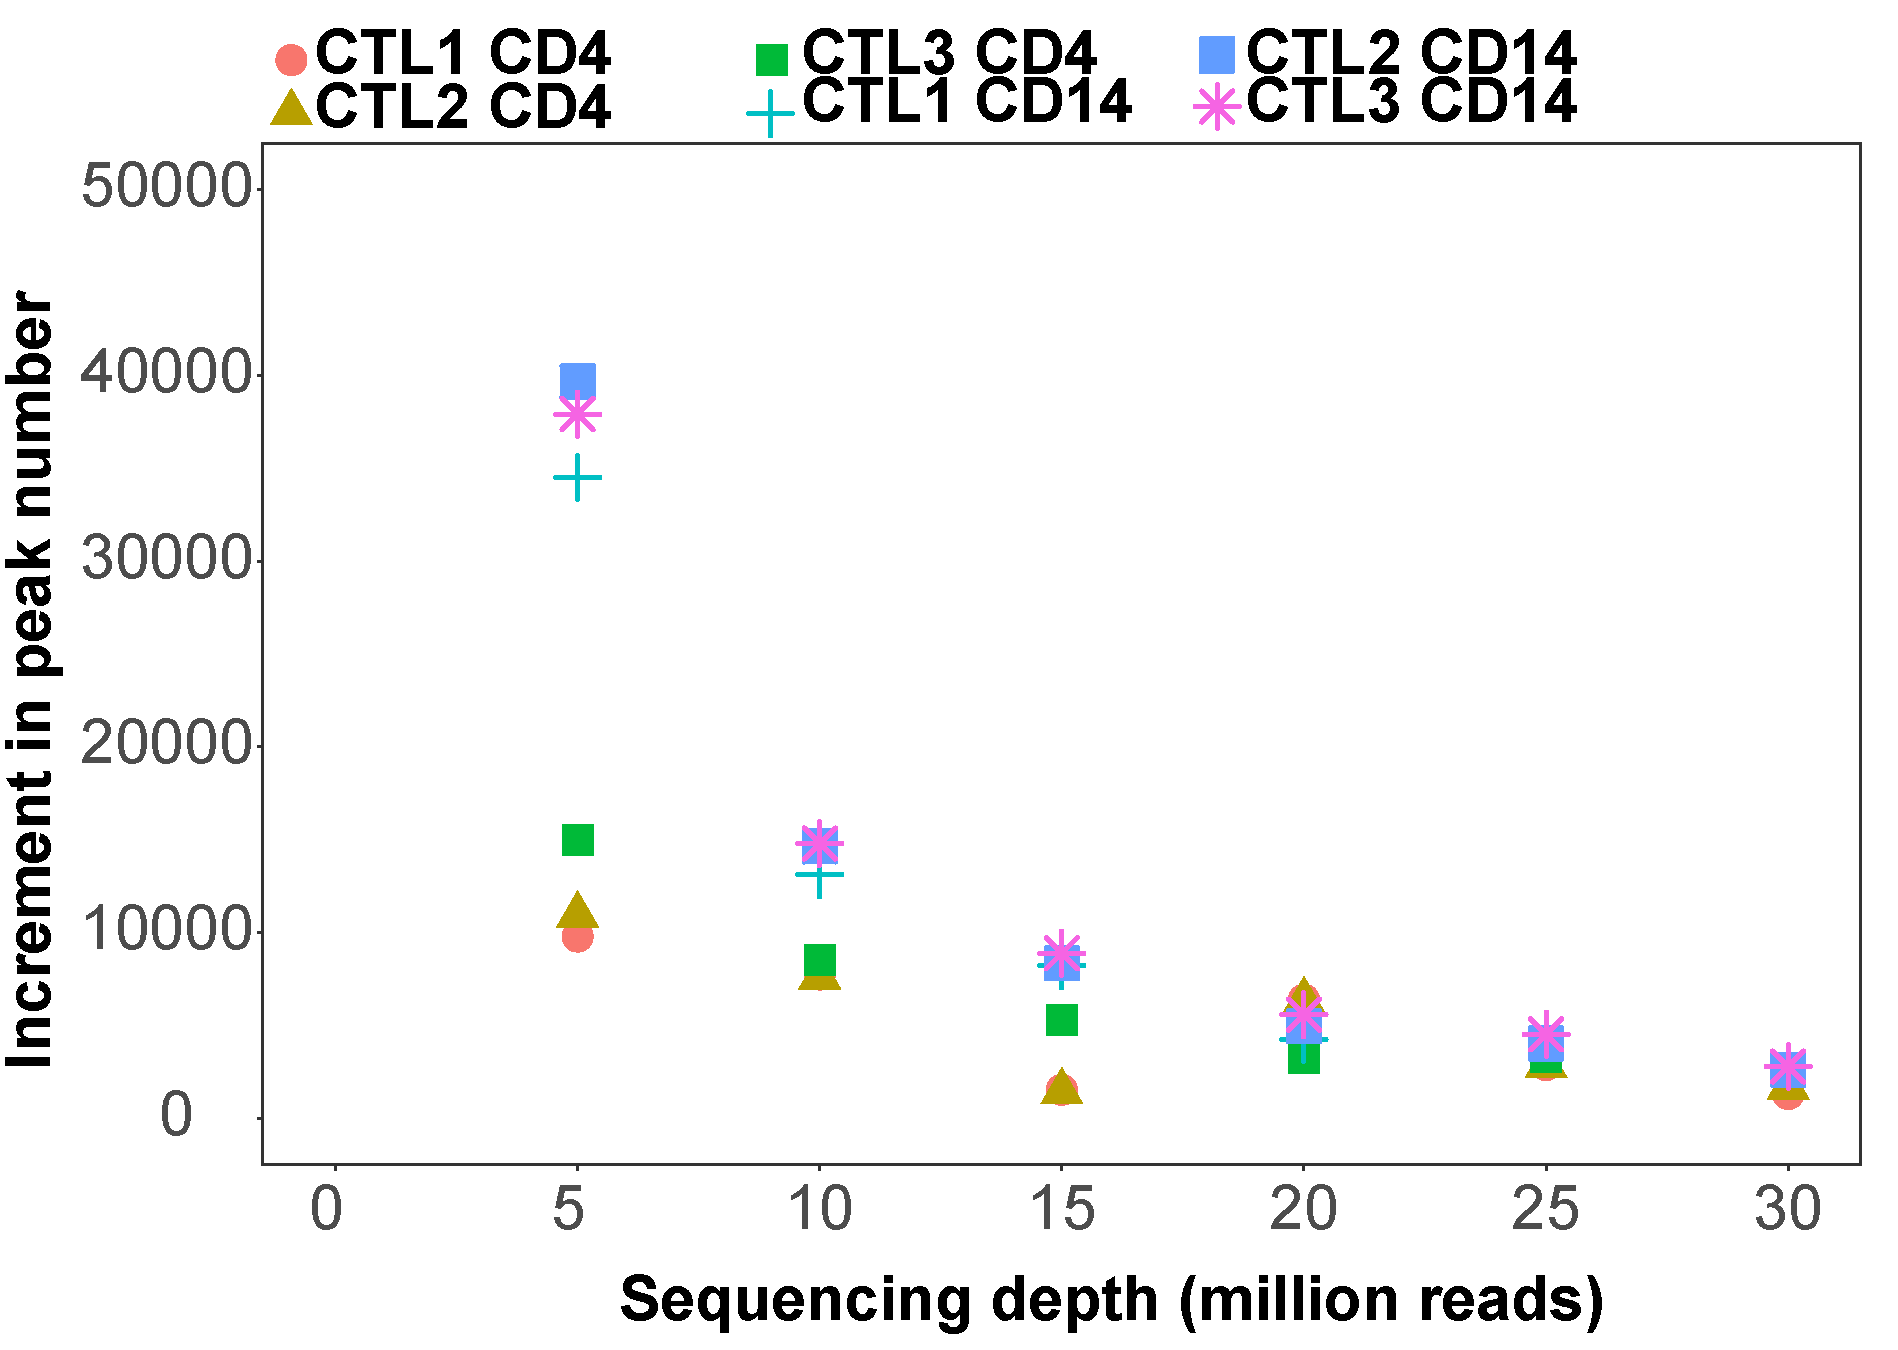
\includegraphics[width=\textwidth]{./Results1/pdfs/ATAC_Core_fresh_CD4_CD14_increment_num_peaks_vs_depth}
\caption{\textbf{}}
\end{subfigure} %
\begin{subfigure}{0.45\textwidth}
\centering
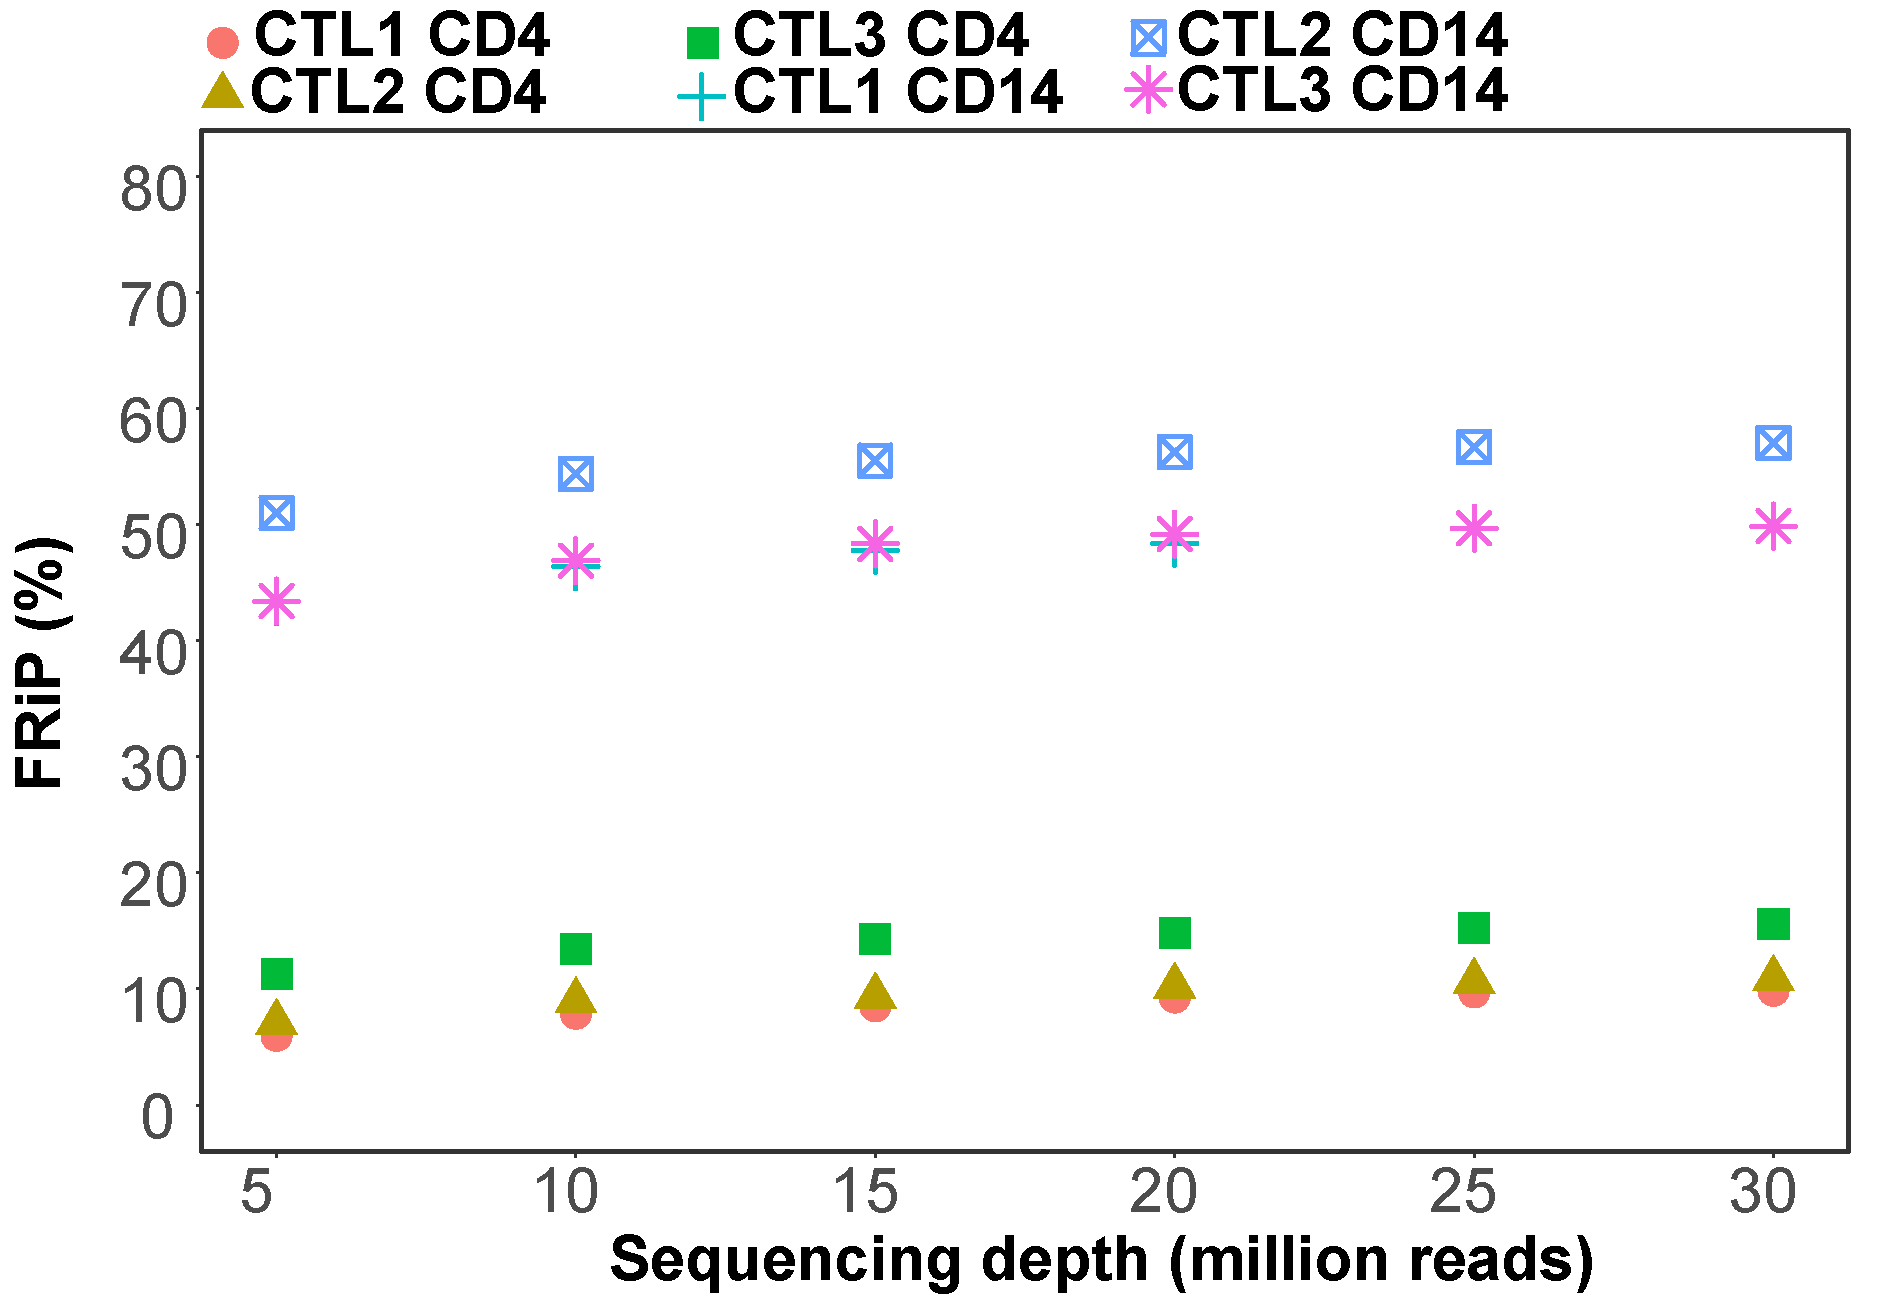
\includegraphics[width=\textwidth]{./Results1/pdfs/ATAC_Core_fresh_CD4_CD14_frac_reads_in_peaks_vs_depth}
\caption{\textbf{}}
\end{subfigure}
\caption[Peak calling and sequencing depth in ATAC-seq samples]{\textbf{Peak calling at different sequencing depth in ATAC-seq samples} \\
}
\label{fig:Peak_calling_versus_depth_ATAC}
\end{figure} 



Regarding peak calling filtering, most of the ATAC-seq publications using MACS2 have arbitrarily used an FDR$<$0.01 (Table \ref{tab:ATAC_comparative_methods}). In collaboration with Dr. Gabriele Migliorini and following ENCODE pipeline, we explored the use of IDR to experimentally identify the most appropriate p-val for filtering each individual sample. Each sample was partitioned in two, peaks were called in each half and the percentage of peaks (over the total number shared peaks) sharing IDR at a particular p-val was calculated (Figure \ref{fig:Peak_calling_IDR_filtering_and_chrom_stated_ATAC} a and b). Both of the representative samples showed variation in the percentage of shared peaks upon sequencing depth under 10M reads, being the effect more pronounced and extended in the lower quality (CTL2 CD4$^+$ Figure \ref{fig:Peak_calling_IDR_filtering_and_chrom_stated_ATAC} a) compared to the counterpart CD14$^+$ (Figure \ref{fig:Peak_calling_IDR_filtering_and_chrom_stated_ATAC} b). The shape of the curves was also influenced by the sample quality, presenting a smoother profile reaching a single maximum percentage of shared IDR peaks for samples with TSS enrichment $>\sim$10 compared to samples with lower quality. All the CD14$^+$ samples reached the maximum percentage of IDR shared peaks at approximately -log10 pval 8 (data not shown). 
Filtering the CD4$^+$ peaks at the -log10 pval of the first maximum of IDR shared peaks reduced the percentage of peaks overlapping noise ( e.g heterochromatin, repetitive sequences and repressed regions) when compared to peaks filtered based on FDR$<$0.01 (Figure \ref{fig:Peak_calling_IDR_filtering_and_chrom_stated_ATAC} b). In summary, this IDR analysis appeared as systematic method to identify an optimum p-val to perform sample-specific filtering of the called peaks used then downstream for building the master list of regions across all the samples to perform chromatin accessibility differential analysis. 

%Should mention that the median of all this first max are used to perform filtering for all the samples because following other pipelines they always use same filtering value for all samples so we need to be consistent across samples



\begin{figure}[htbp]
\centering
\begin{subfigure}{0.5\textwidth}
\centering
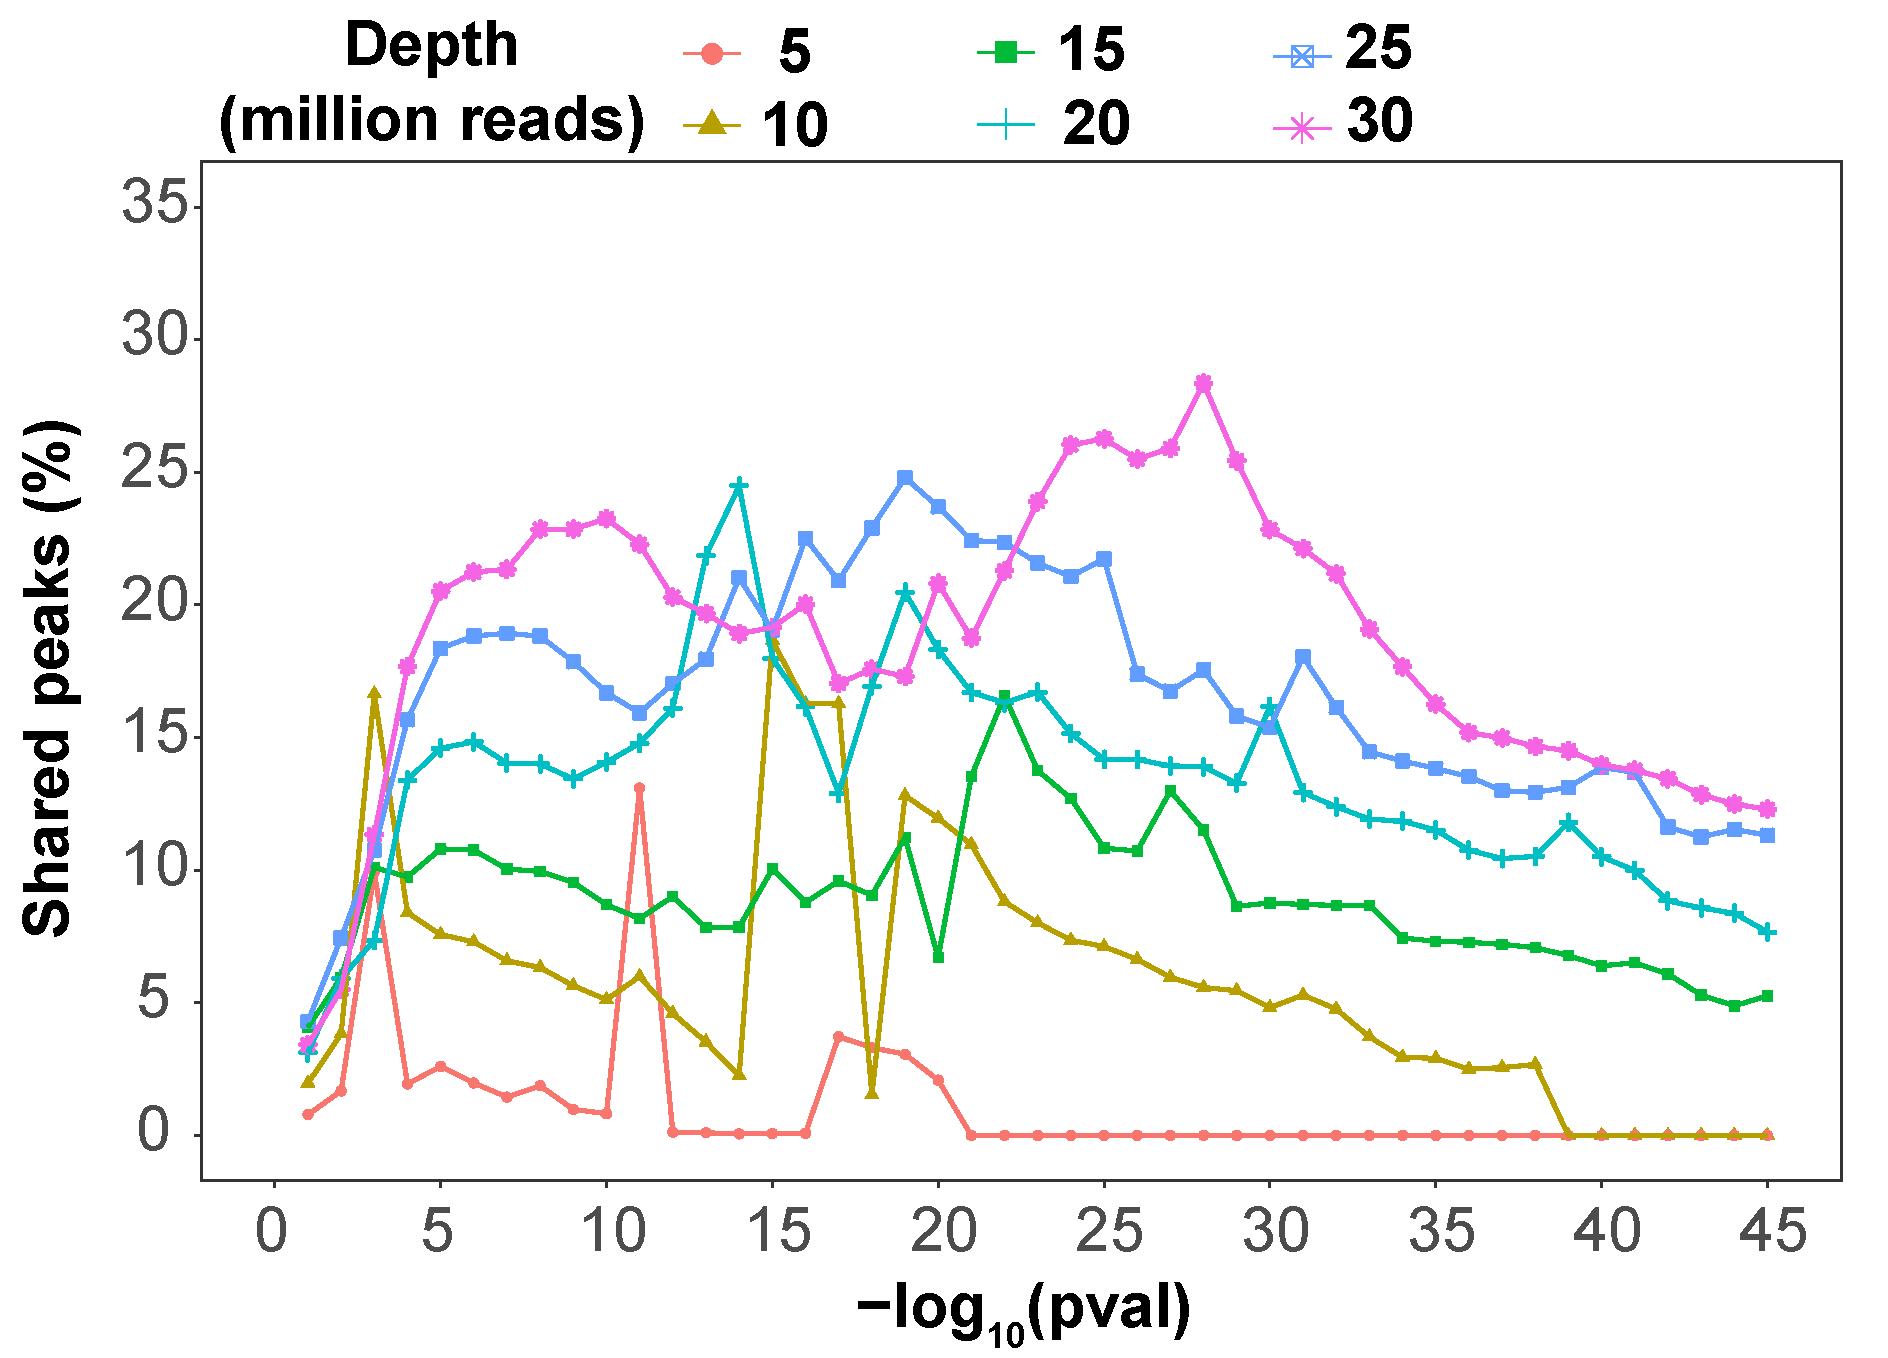
\includegraphics[width=\textwidth]{./Results1/pdfs/ATAC_Core_fresh_CTL2_CD4_shared_peaks_IDR_vs_pval}
\caption{\textbf{}}
% The percentage sign indicated that the other subfig goes side by side
\end{subfigure}%
\begin{subfigure}{0.5\textwidth}
\centering
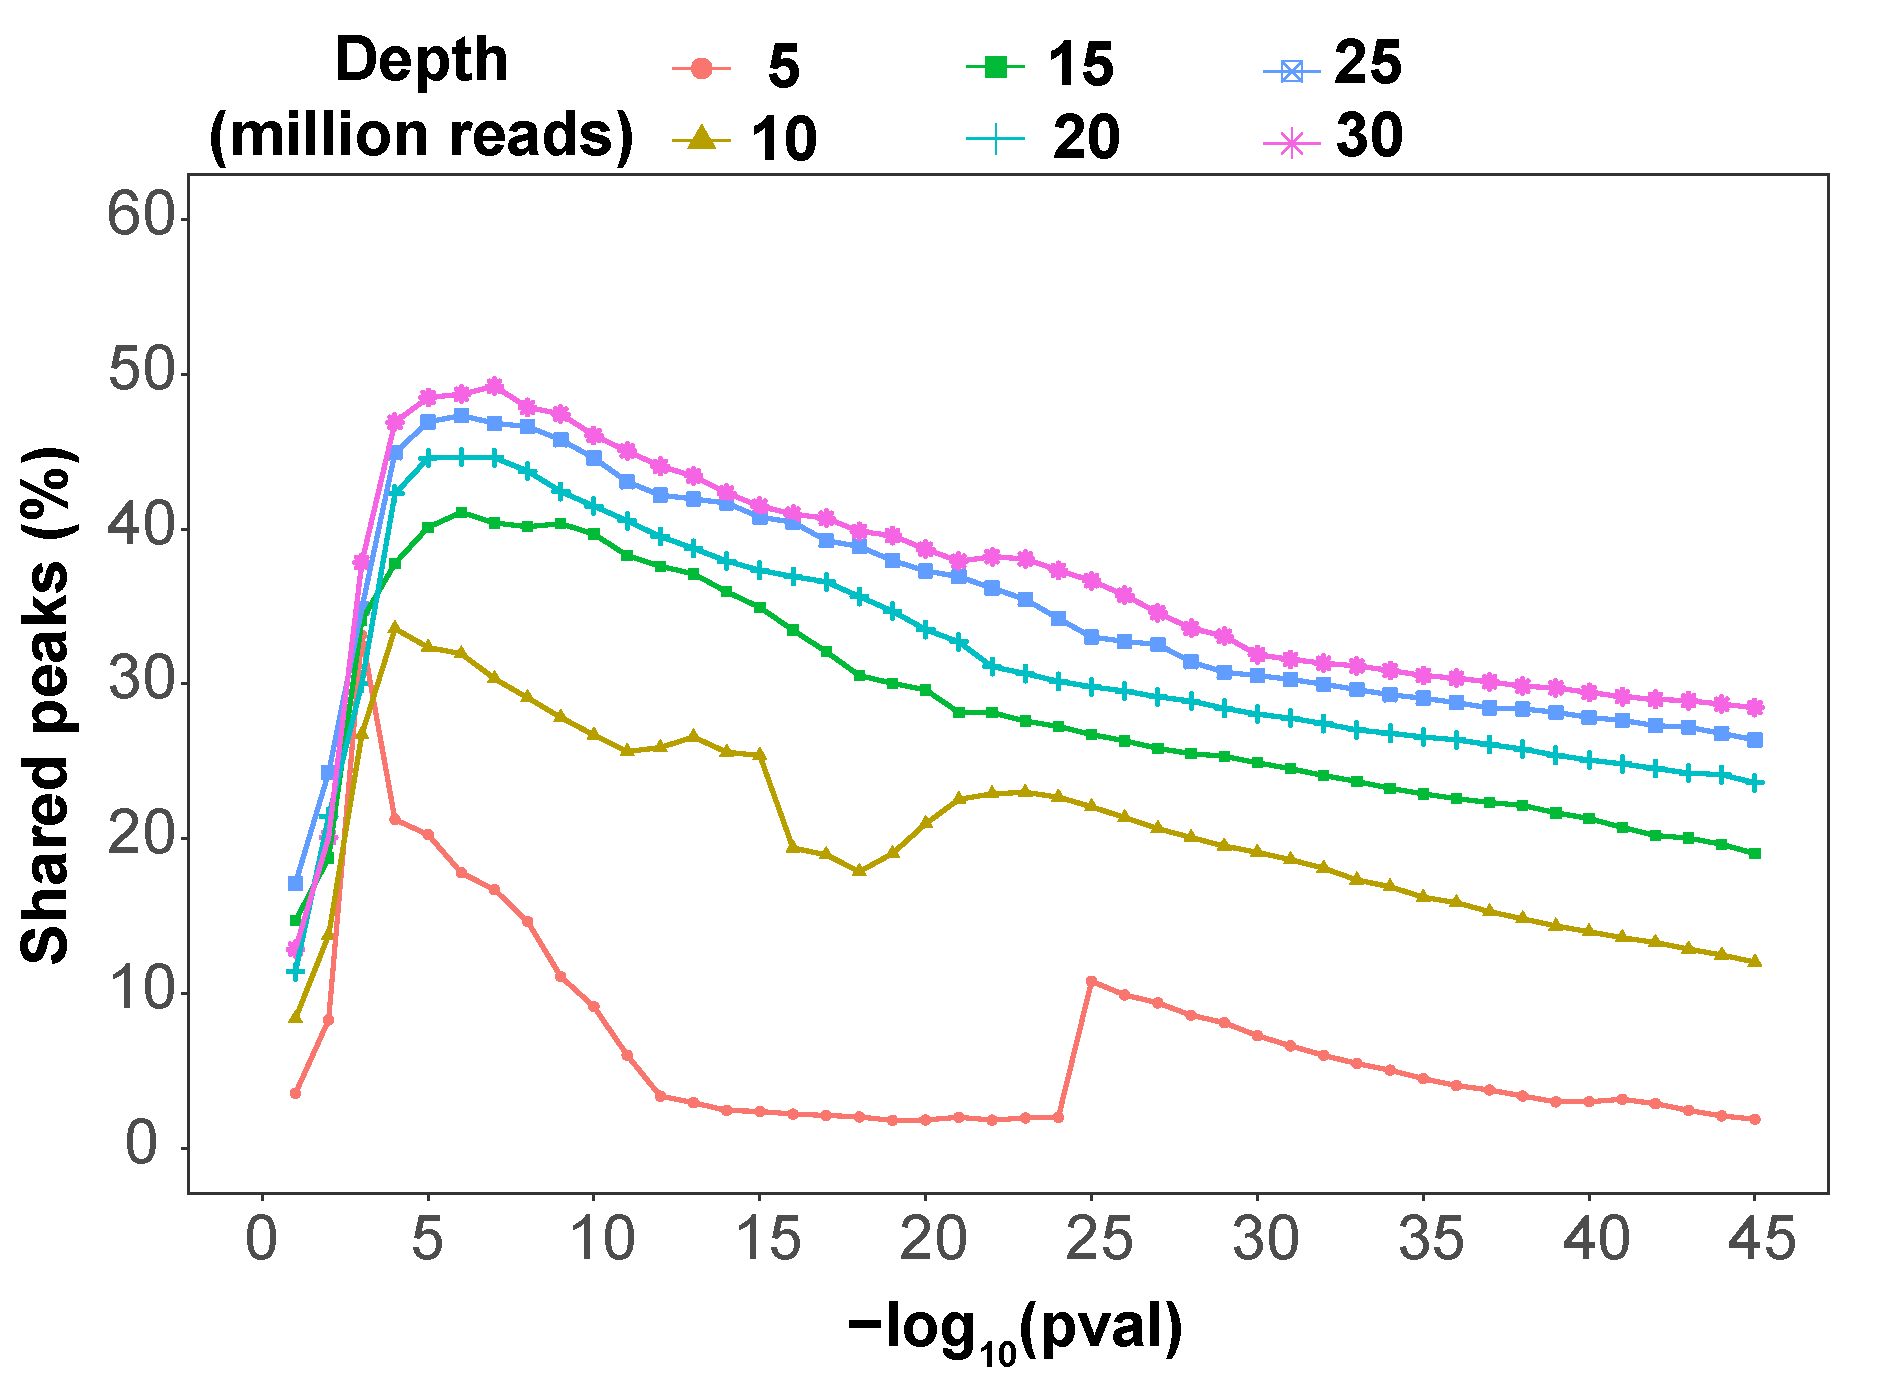
\includegraphics[width=\textwidth]{./Results1/pdfs/ATAC_Core_fresh_CTL2_CD14_shared_peaks_IDR_vs_pval}
\caption{\textbf{}}
\end{subfigure} \\
\begin{subfigure}{0.65\textwidth}
\centering
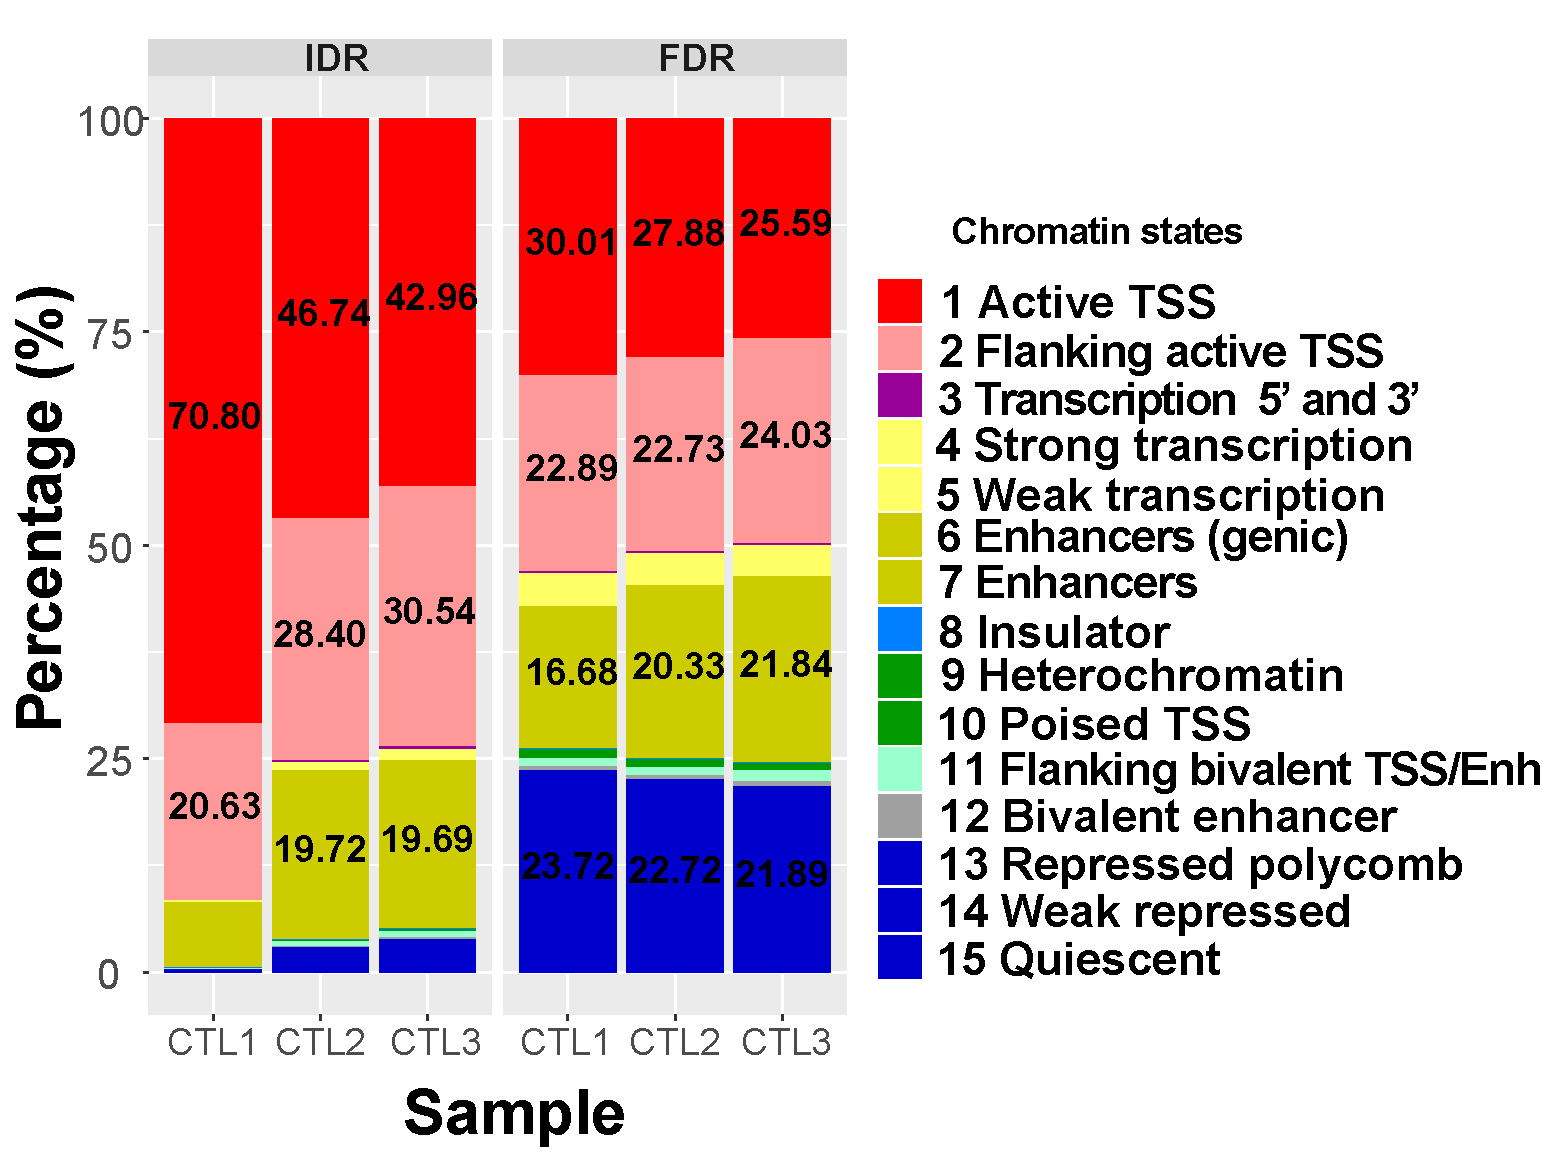
\includegraphics[width=\textwidth]{./Results1/pdfs/stacked_barplot_chromatin_states_percent_CD4_qval_vs_PVAL_IDR_filtered}
\caption{\textbf{}} % to add text to the figure name
\end{subfigure}%
\caption[Peak calling filtering using IDR analysis in ATAC-seq samples]{\textbf{Peak calling filtering using IDR analysis in ATAC-seq samples}}
\label{fig:Peak_calling_IDR_filtering_and_chrom_stated_ATAC}
\end{figure} 




\subsubsection{Differential chromatin accessibility analysis}

From the methods that can be used to perform differential chromatin accessibility analysis (Table \ref{tab:ATAC_comparative_methods}), I chose a peak-based approach where a consensus master list between all samples was built and the number of reads overlapping the master list peaks were retrieved for each sample. As previously mentioned in the Chapter \label{ch:Mat} the master list was composed of non-overlapping 500bp with peaks present in at least 30\% of the samples, regardless the group they belonged to (e.g patients or controls). One of the main limitations of the ATAC-seq and FAST-ATAC protocols (discussed in the next section) is the background signal. Therefore, it was calculation of an empirical cut-off, similarly to the strategy use in micro-array technology, was performed to minimise the impact of background read counts on the differential analysis \parencite{Xinmin2005,Jonker2014}. Moreover, due to the lack of consistency found across the ATAC-seq publications, two methods for normalisation/differential analysis were assayed.

From the count matrix of the same six samples as before, the combined distribution of read density from all the absent peaks in each sample was used to define a sequence of twenty cut-offs. These cut-offs corresponded to the number of counts showed by a particular percentage of absent peaks (supplementary info). Each cut-off was used to filter out from the raw count matrix those peaks from the master list for which the number of counts was $<=$ than that particular cut-off in more than three samples  (being three the number of the smallest group of replicates in this particular experimental design). Quantile normalisation followed by differential analysis with limma voom showed greater number of differential open chromatin regions (DOCs) at an FDR$<$0.01 compared to DESeq2 across all the cut-offs (Figure \ref{fig:DOC_quantile_DESeq2} a). The two approaches presented progressive decrease in the number of DOC sites from the 75\% cut-off. Conversely, the proportion of DOC calculated over the total number of regions considered in the differential analysis for each cut off significantly increased from the 50\% cut-off onwards, indicating a progressive reduction in the false positive hits reported \ref{fig:DOC_quantile_DESeq2} b). 
From this analysis, 80\% was chosen as a conservative filtering cut-off for which almost all the 19,855 DOCs identified by the most conservative method (DESeq2) at an FDR$<$0.01 were recapitulated by limma voom at the same FDR (Figure \ref{fig:DOC_quantile_DESeq2} c). 

\begin{figure}[htbp]
\centering
\begin{subfigure}{0.45\textwidth}
\centering
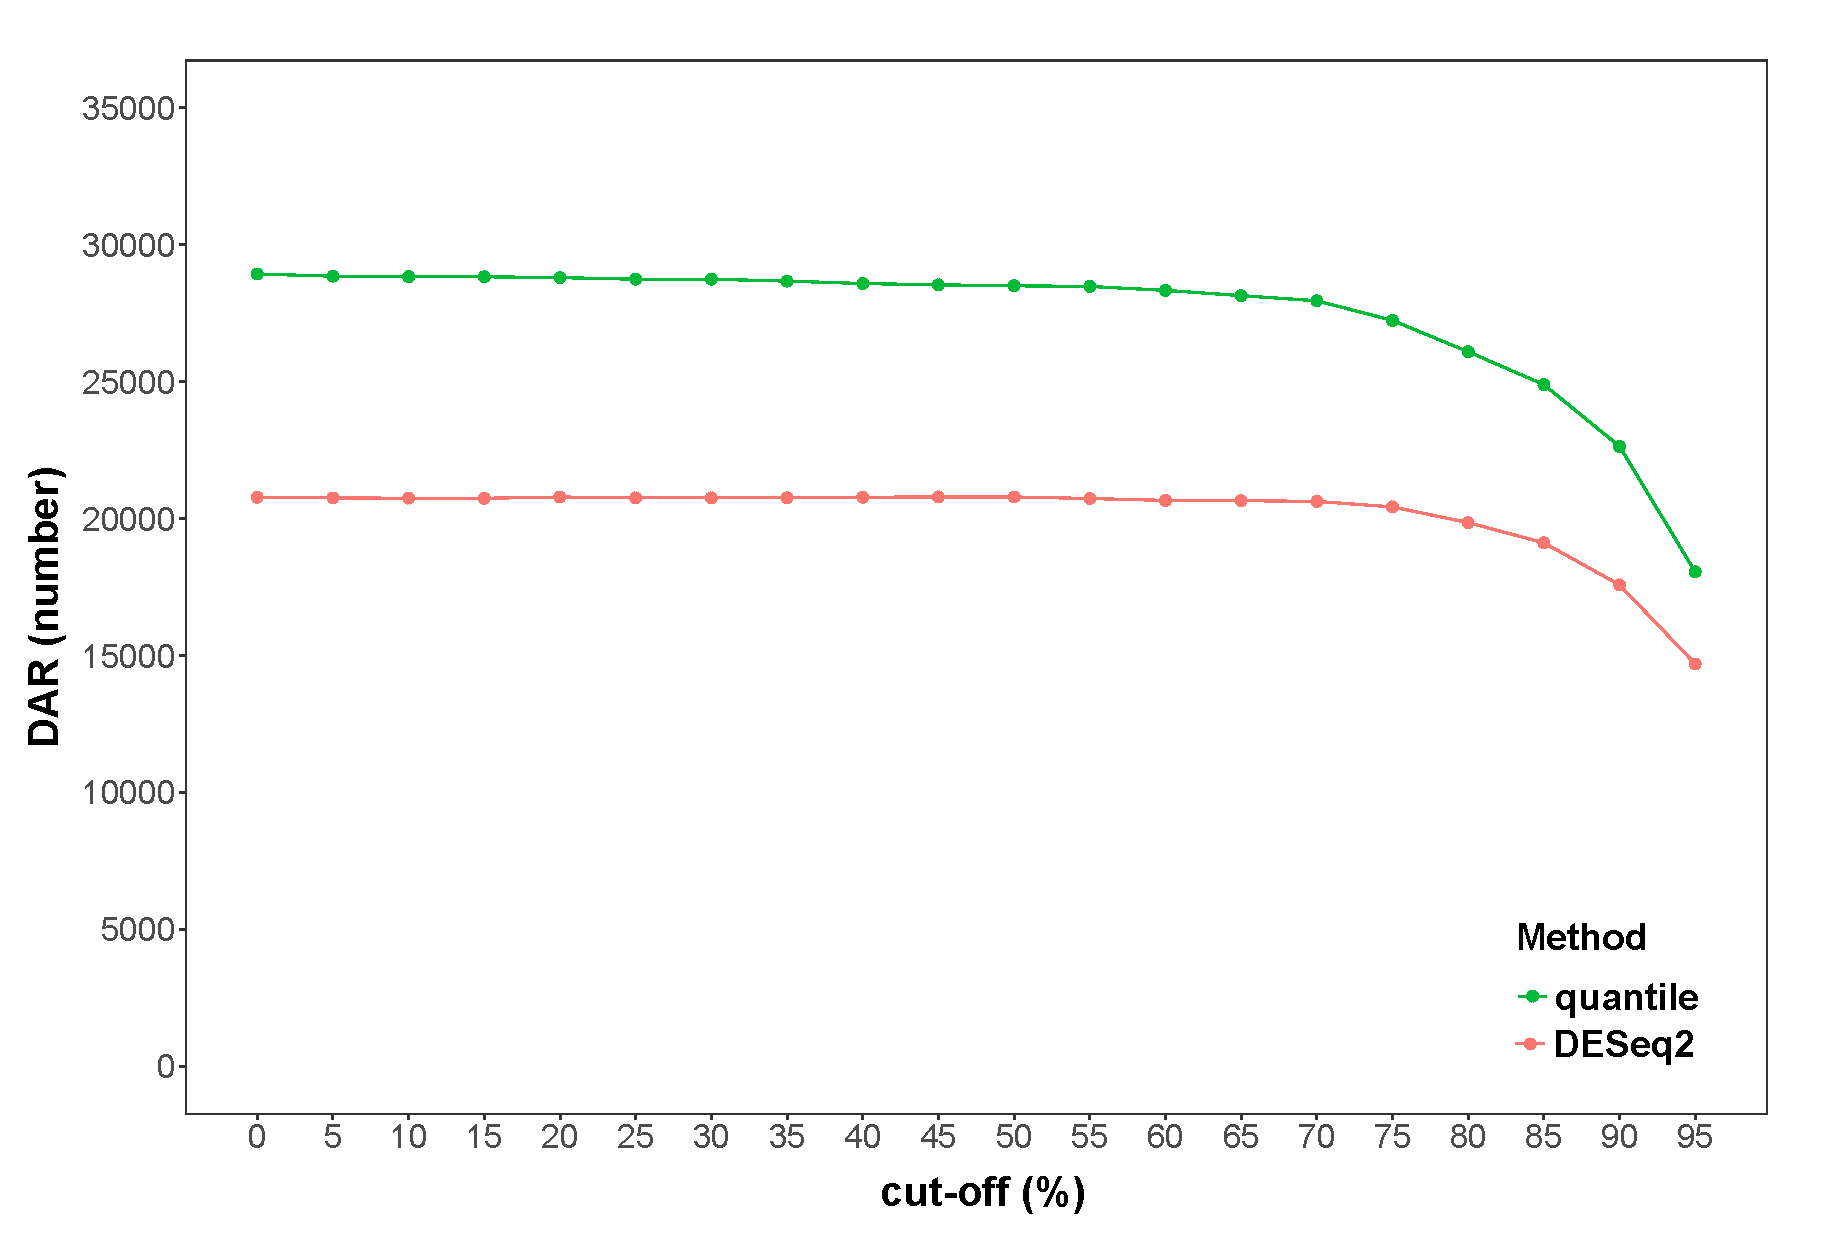
\includegraphics[width=\textwidth]{./Results1/pdfs/ATAC_Core_CD4vsCD14_DOC_FDR_01_vs_cutoffs_quantile_DESeq2_only}
\caption{\textbf{}}
\end{subfigure}%
\begin{subfigure}{0.45\textwidth}
\centering
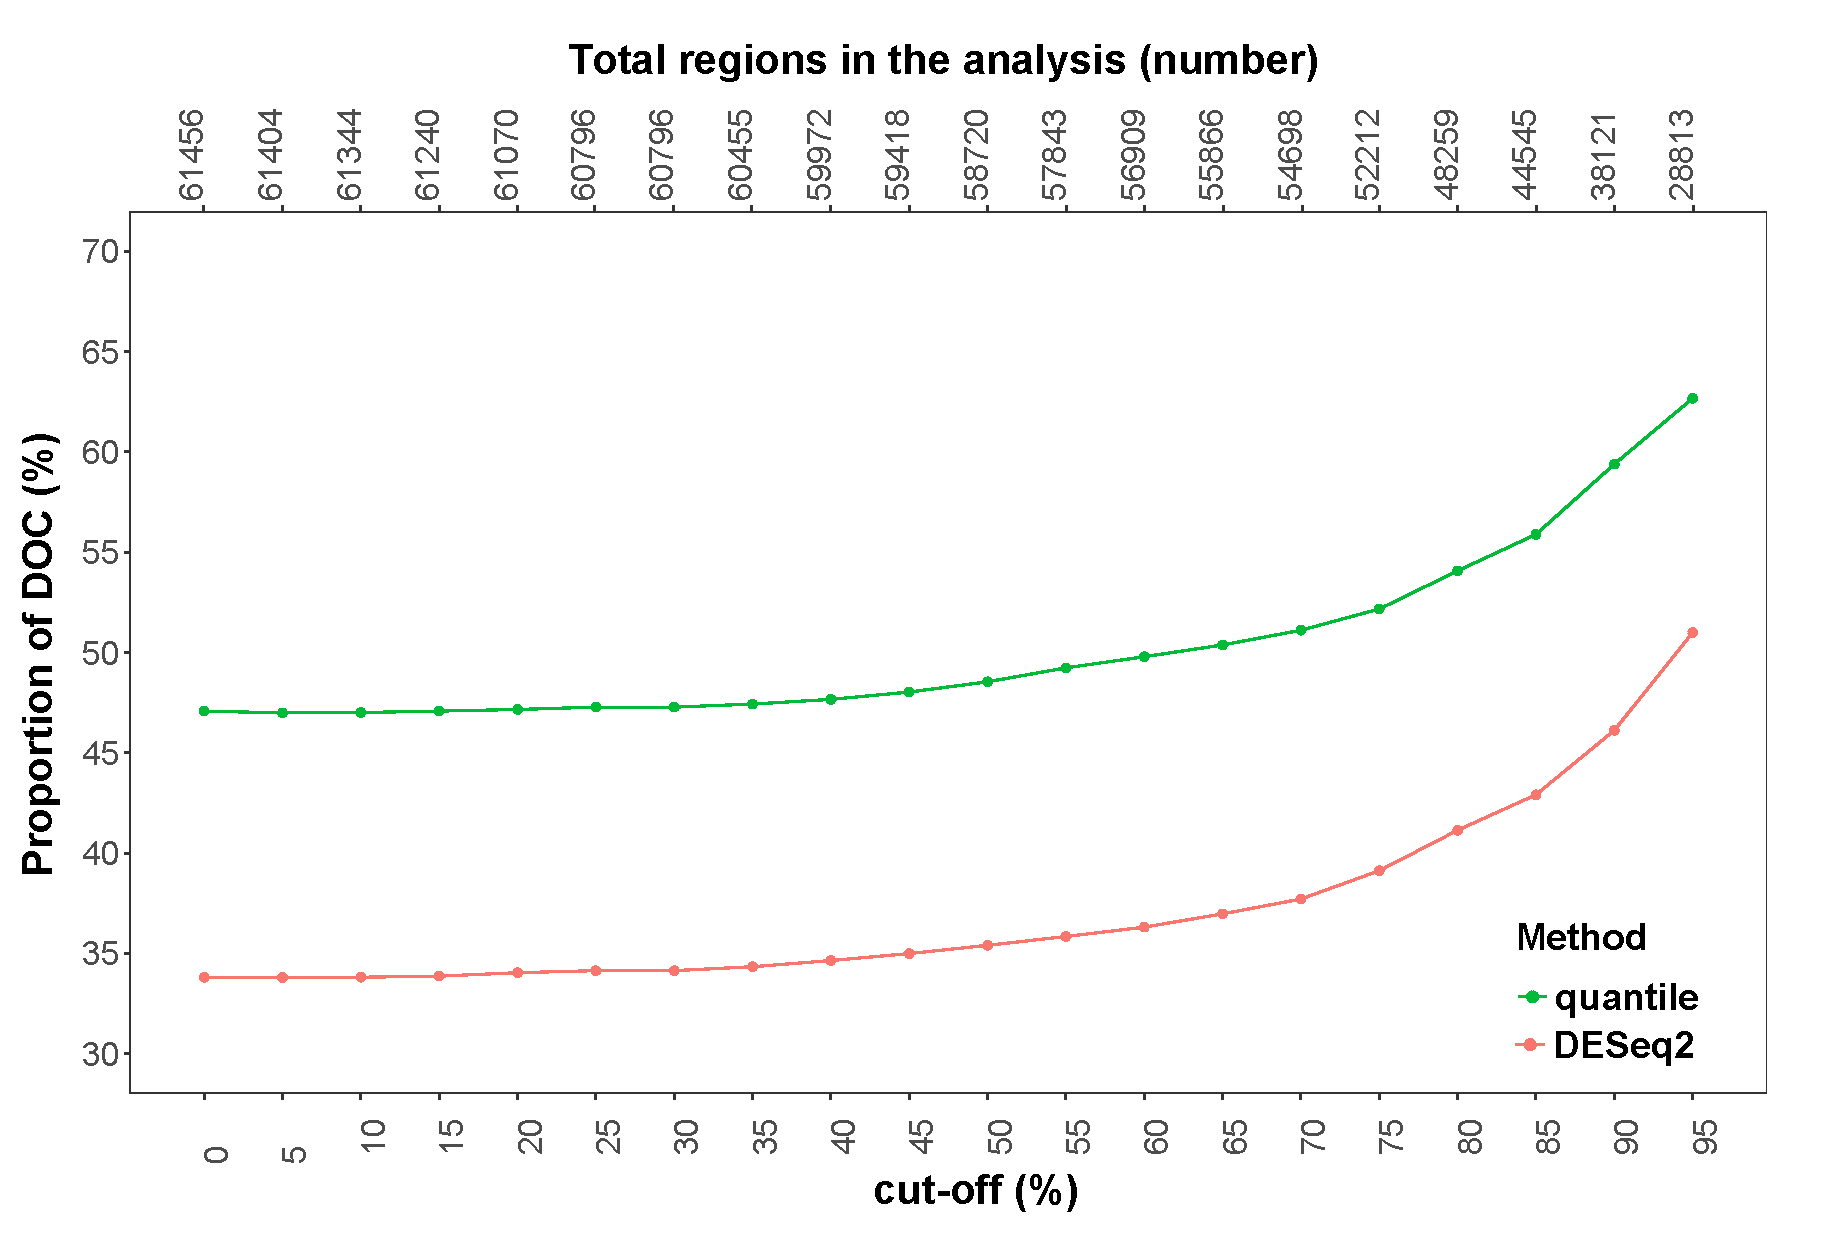
\includegraphics[width=\textwidth]{./Results1/pdfs/ATAC_Core_CD4vsCD14_proportion_DOC_FDR_01_vs_cutoffs_quantile_DESeq2_only}
\caption{\textbf{}}
\end{subfigure}
\begin{subfigure}{0.5\textwidth}
\centering
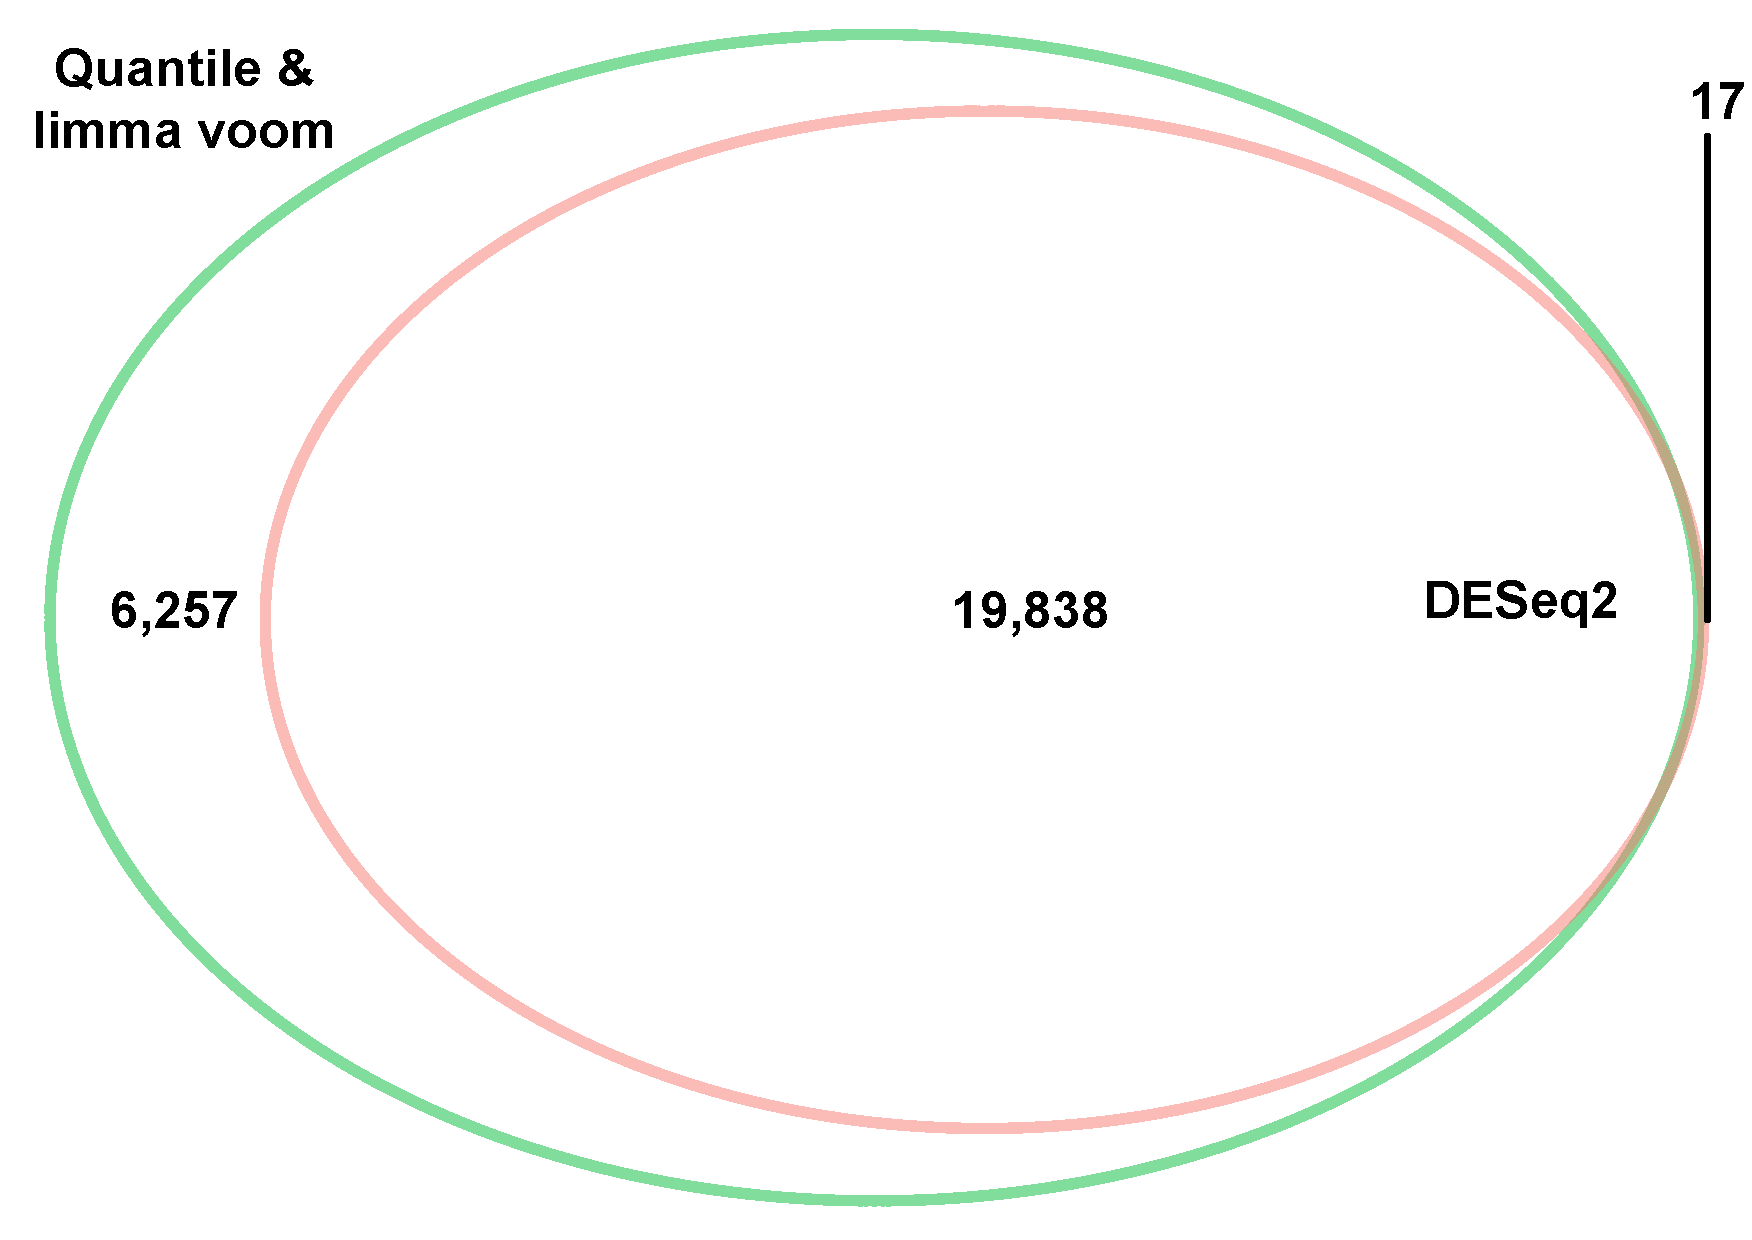
\includegraphics[width=\textwidth]{./Results1/pdfs/ATAC_Core_fresh_CD4vsCD14_venn_diagram_differential_analysis_FDR_01_quantile_DESeq2_only}
\caption{\textbf{}} % to add text to the figure name
\end{subfigure}%
\caption[Differential chromatin accessibility analysis for different background reads cut-offs.]{\textbf{Differential chromatin accessibility analysis using limma voom and DESeq2.\\
}}
\label{fig:DOC_quantile_DESeq2}
\end{figure} 


Both methods performed appropriate normalisation of the counts at each of the master list peaks across the six samples, being the median of the quantile normalisation slightly more consistent across the two cell types compared to DESeq2 (Figure \ref{fig:QC_quantile_DOC_and_DESeq2_comparison} a). When looking at the first FDR ranked 19,855 limma voom DOCs, 18,768 of them were the same as the retrieved by DESeq2. Moreover, very significant positive correlation was found between the fold changed of those 18,768 significant DOCs in both differential analysis methods (r$^2$=0.999, p-val=2.2$^-16$) (Figure \ref{fig:QC_quantile_DOC_and_DESeq2_comparison} b). These observations suggested that the differences in the number of FDR significant DOCs reported by each of the methods could be partly due to differences in the way of calculating the false-positive rate.

 
Clustering and heat map and pathway analysis-briefly


\begin{figure}[htbp]
\centering
\begin{subfigure}{0.48\textwidth}
\centering
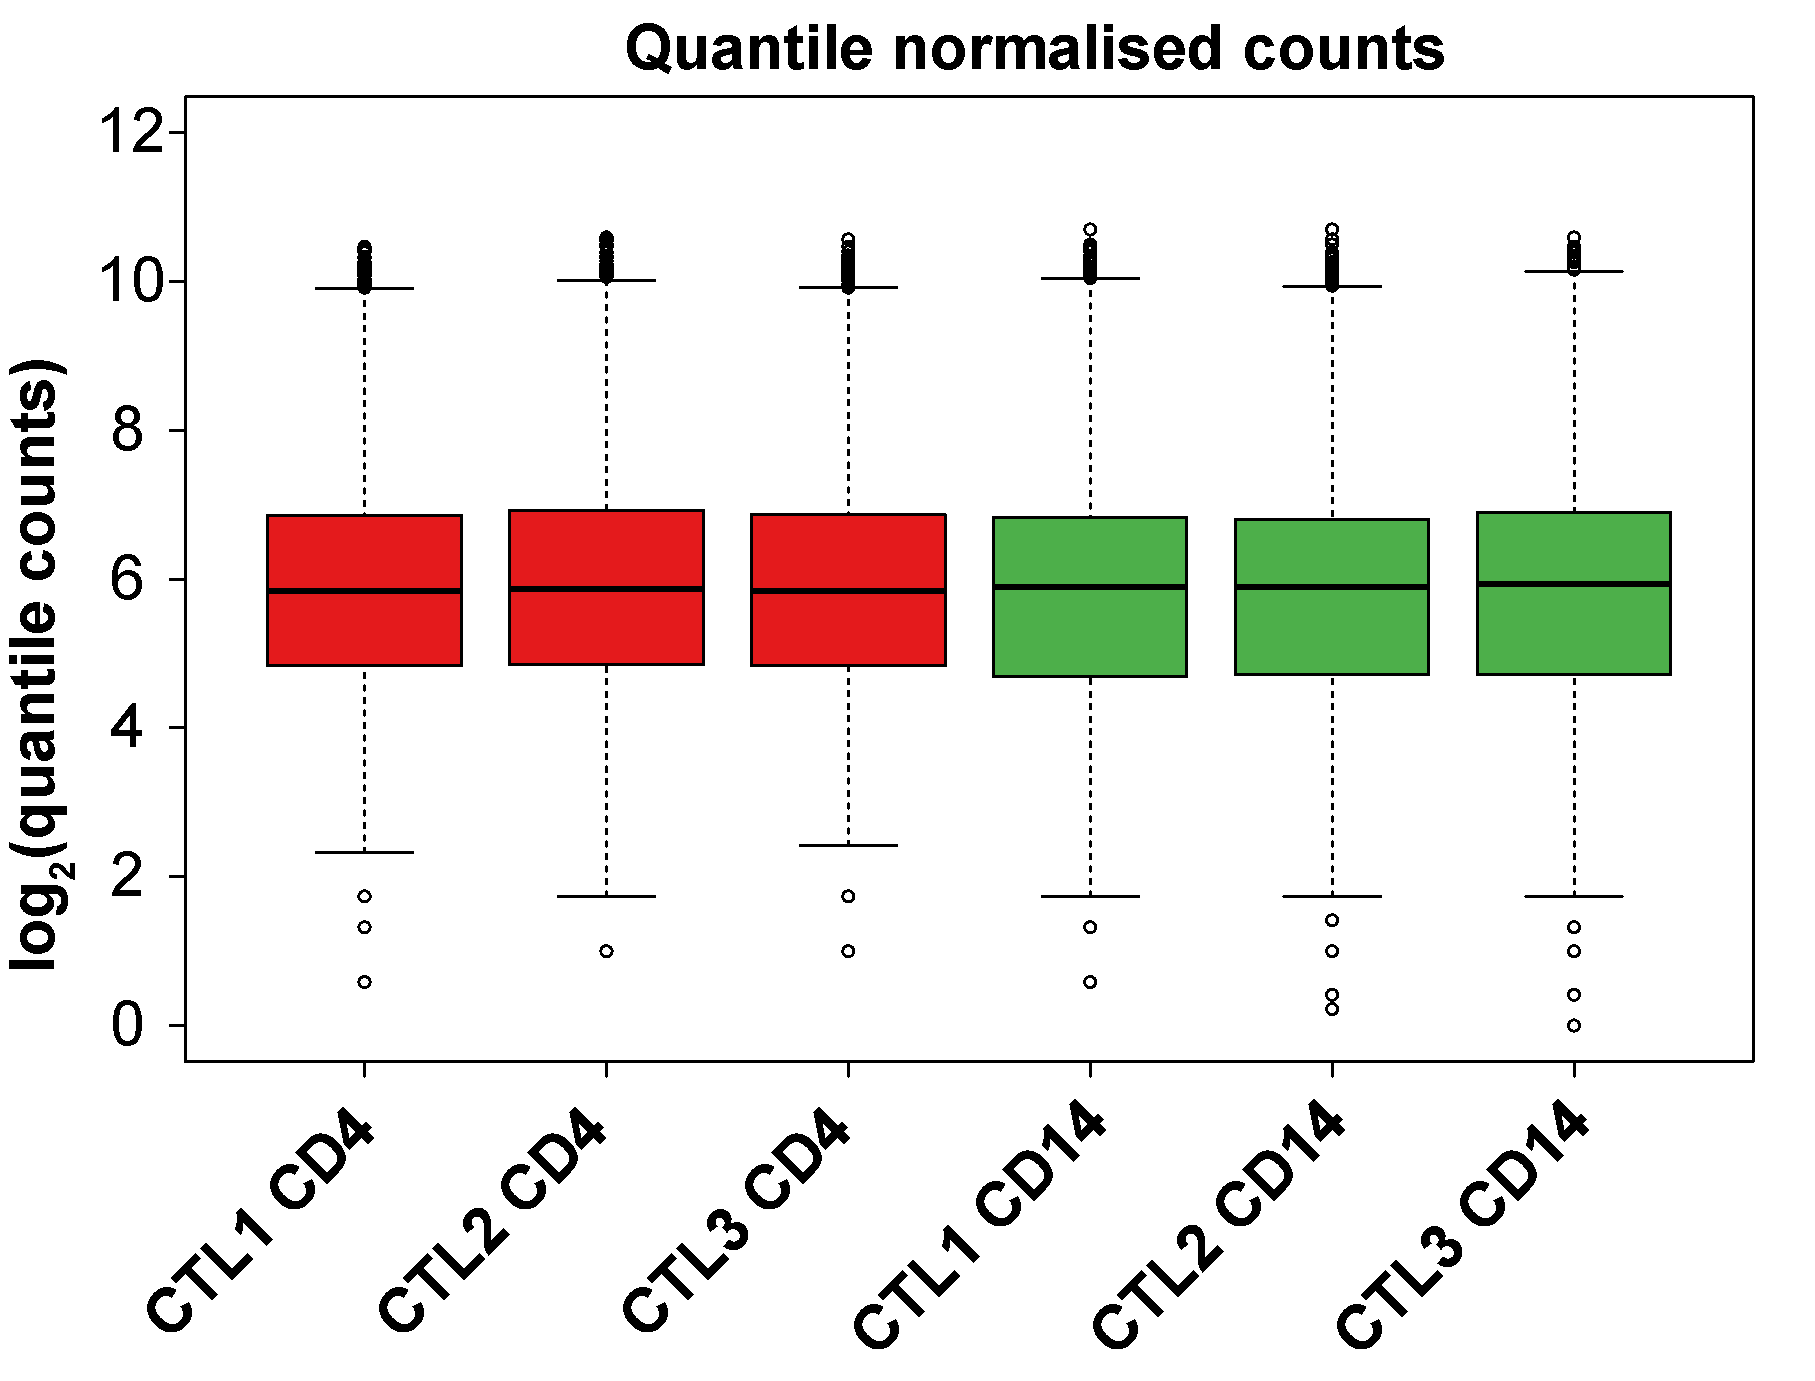
\includegraphics[width=\textwidth]{./Results1/pdfs/ATAC_Core_CD4_CD14_boxplot_80pcnt_cut_off_filtered_quantile_counts}
\caption{\textbf{}}
\end{subfigure}%
\begin{subfigure}{0.48\textwidth}
\centering
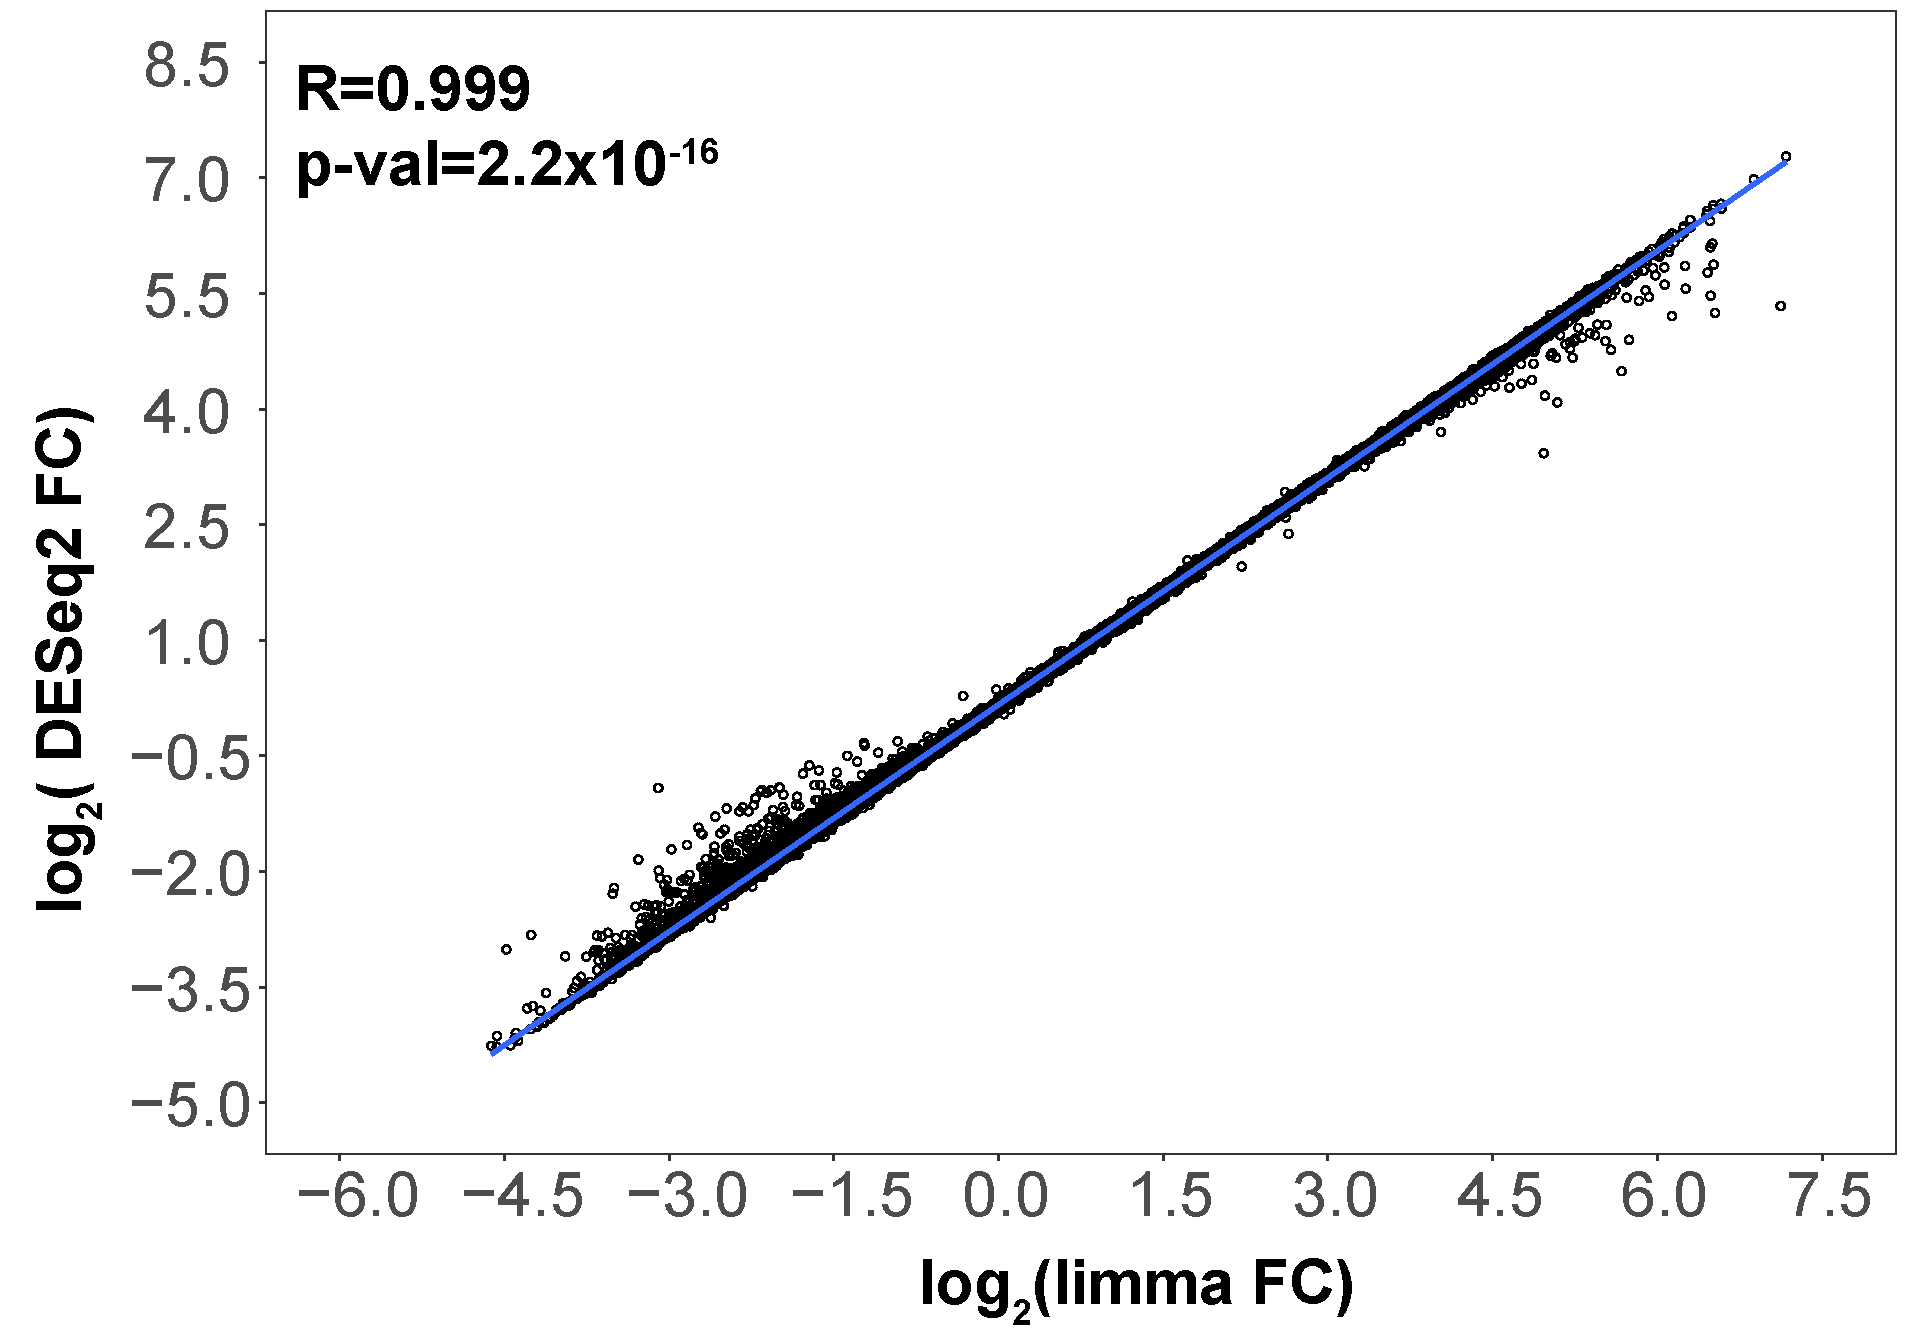
\includegraphics[width=\textwidth]{./Results1/pdfs/ATAC_Core_fastq_CD4_CD14_80pcnt_cut_off_correlation_log2FC_quantile_vs_deseq2}
\caption{\textbf{}}
\end{subfigure}
\begin{subfigure}{0.65\textwidth}
\centering
\includegraphics[width=\textwidth]{./Results1/pdfs/ATAC_Core_CD4vsCD14_clusters_and_heatmap_quantile_common}
\caption{\textbf{}} % to add text to the figure name
\end{subfigure}
\caption[Exploration of the differential chromatin accessibility analysis using 80\% as the empirical cut-off.]{\textbf{Exploration of the differential chromatin accessibility analysis using 80\% as the empirical cut-off.}}
\label{fig:QC_quantile_DOC_and_DESeq2_comparison}
\end{figure} 


\subsection{Assessment of ATAC-seq transposition times and comparison with FAST-ATAC protocol in relevant cell types}


\begin{figure}[htbp]
\centering
\begin{subfigure}{0.5\textwidth}
\centering
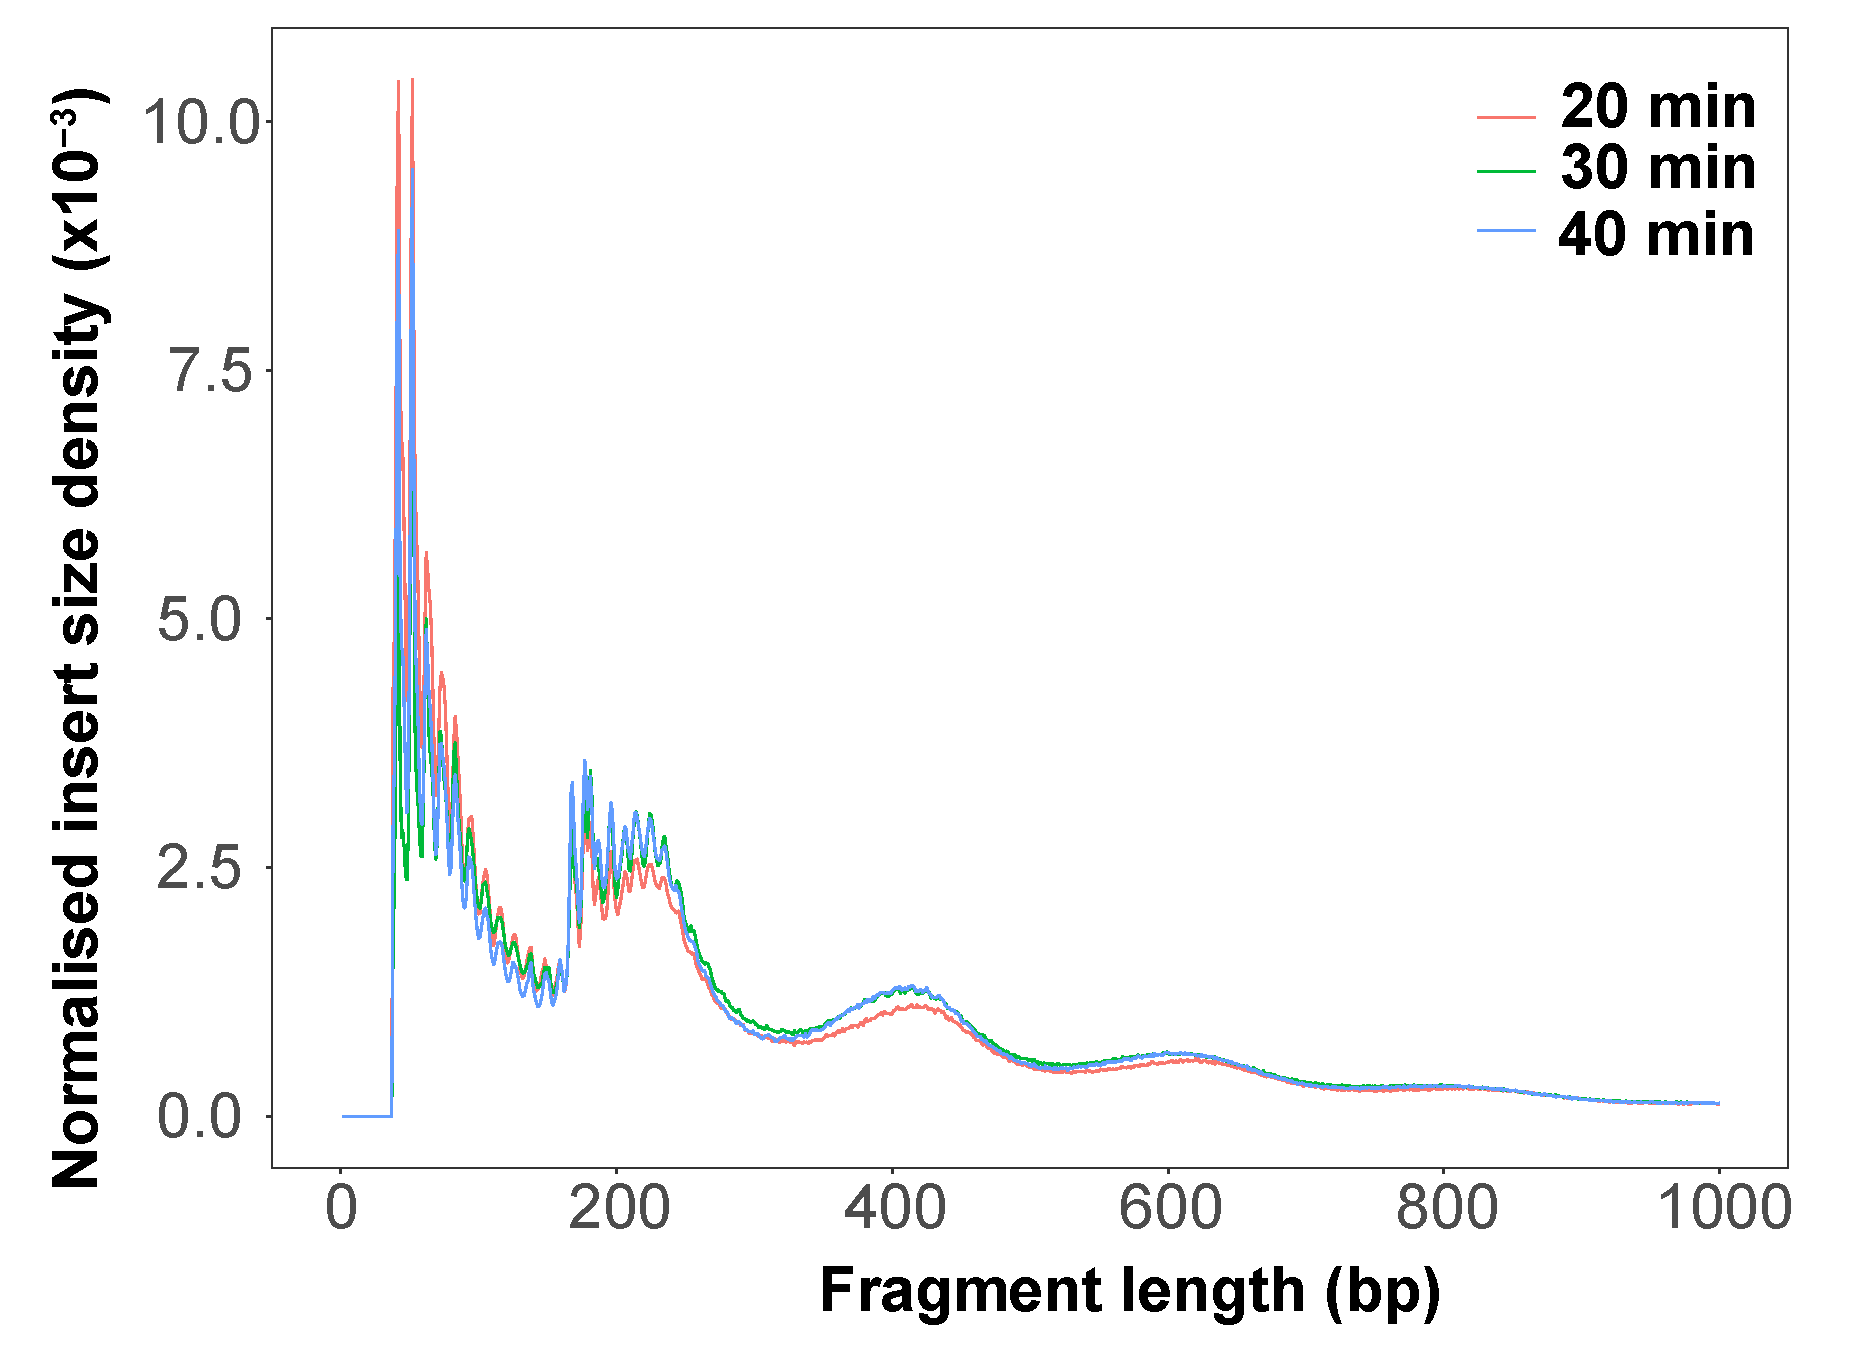
\includegraphics[width=\textwidth]{./Results1/pdfs/ATAC_CD8_fragment_size_distribution_20_30_40min}
\caption{\textbf{}}
% The percentage sign indicated that the other subfig goes side by side
\end{subfigure}
\begin{subfigure}{0.5\textwidth}
\centering
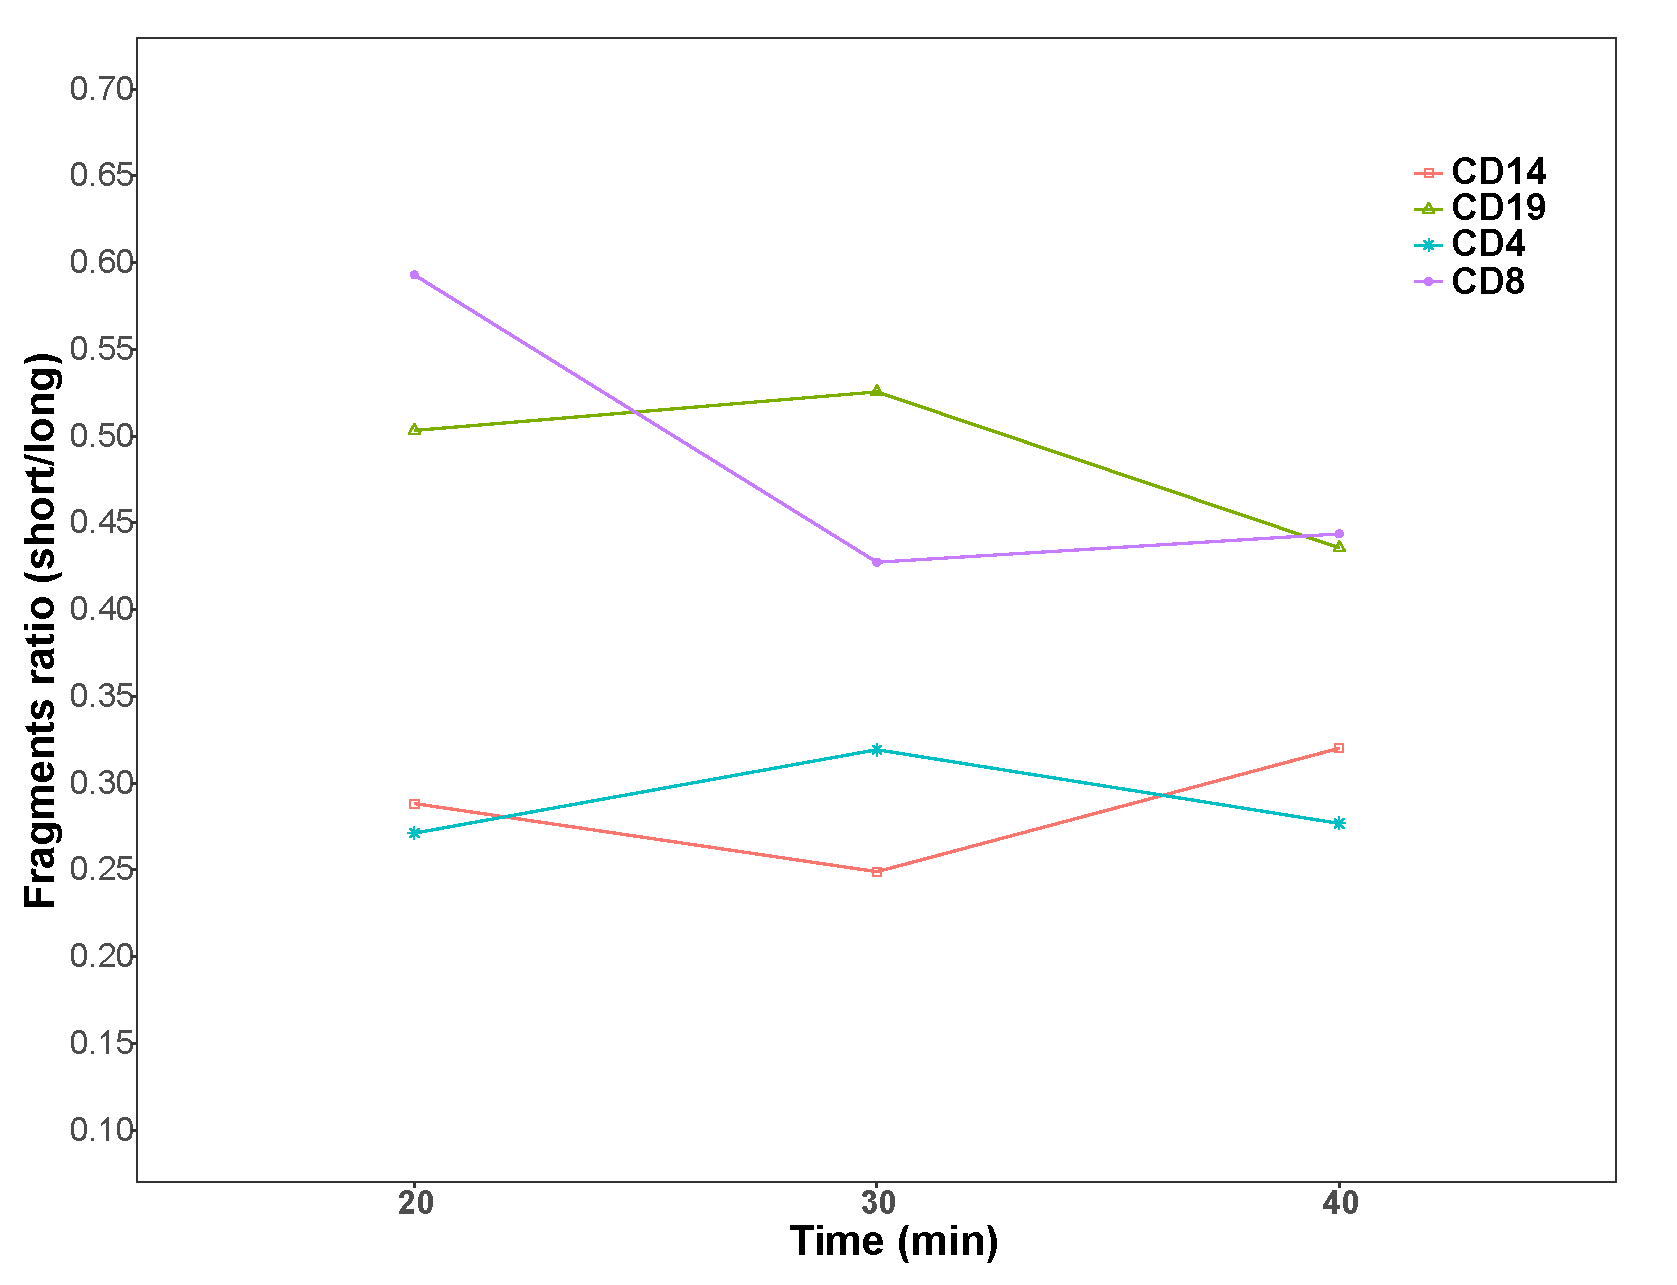
\includegraphics[width=\textwidth]{./Results1/pdfs/ATAC_ratio_short_long_fragments_20_30_40_min}
\caption{\textbf{}}
\end{subfigure} \\
\begin{subfigure}{0.5\textwidth}
\centering
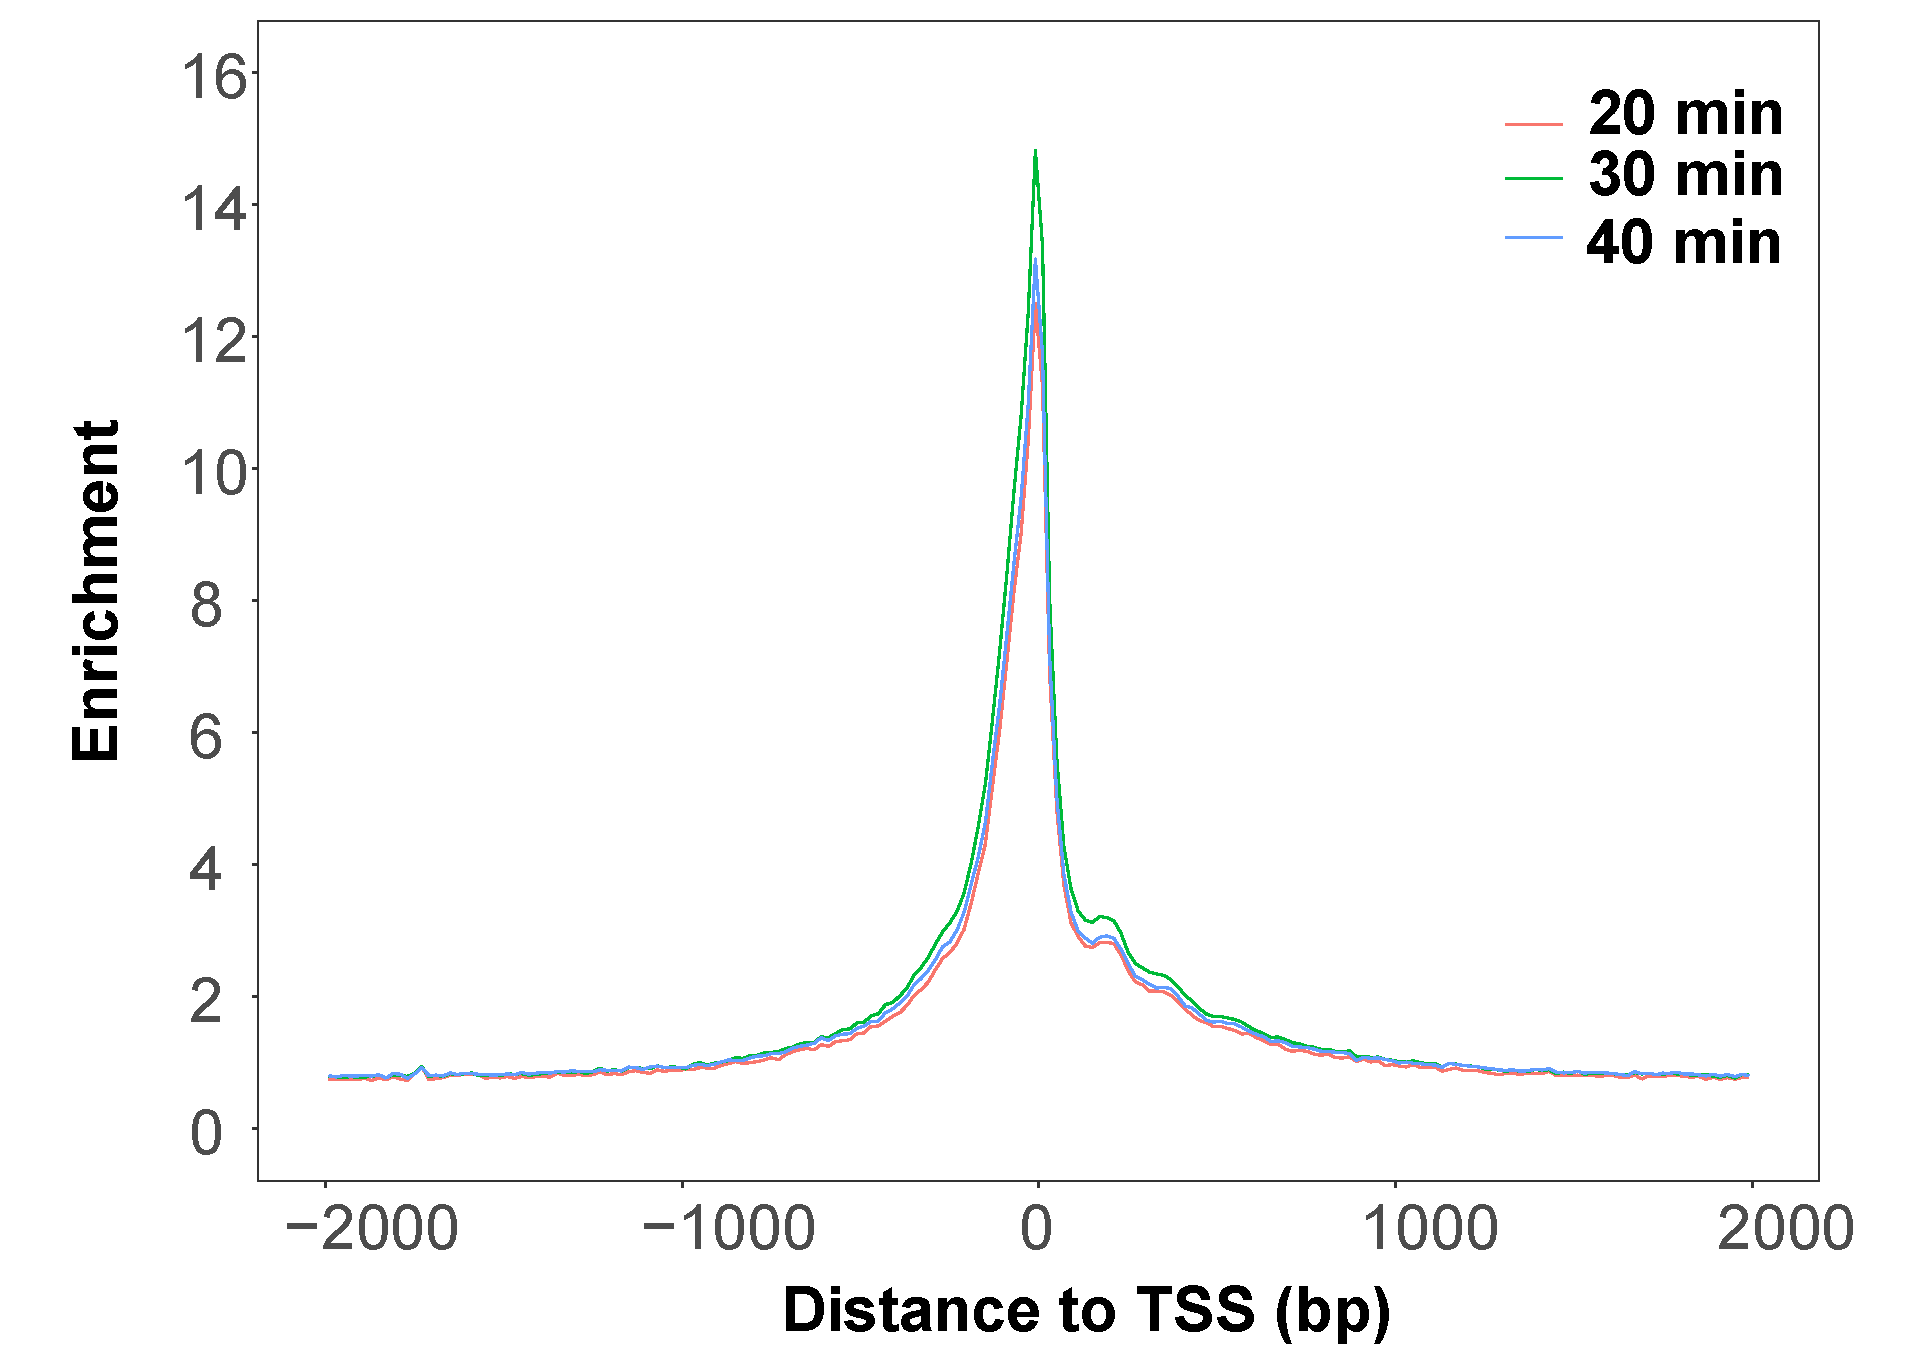
\includegraphics[width=\textwidth]{./Results1/pdfs/ATAC_optimisation_CD4_20_30_40_min_tss_enrichment}
\caption{\textbf{}} % to add text to the figure name
\end{subfigure}
\caption[Assessment of the effect of transposition times on the ATAC-seq QC parameters]{\textbf{Assessment of the effect of transposition times on the ATAC-seq QC parameters} \\
}
\label{fig:Transposition_times_ATAC}
\end{figure} 



\begin{figure}[htbp]
\centering
\begin{subfigure}{0.5\textwidth}
\centering
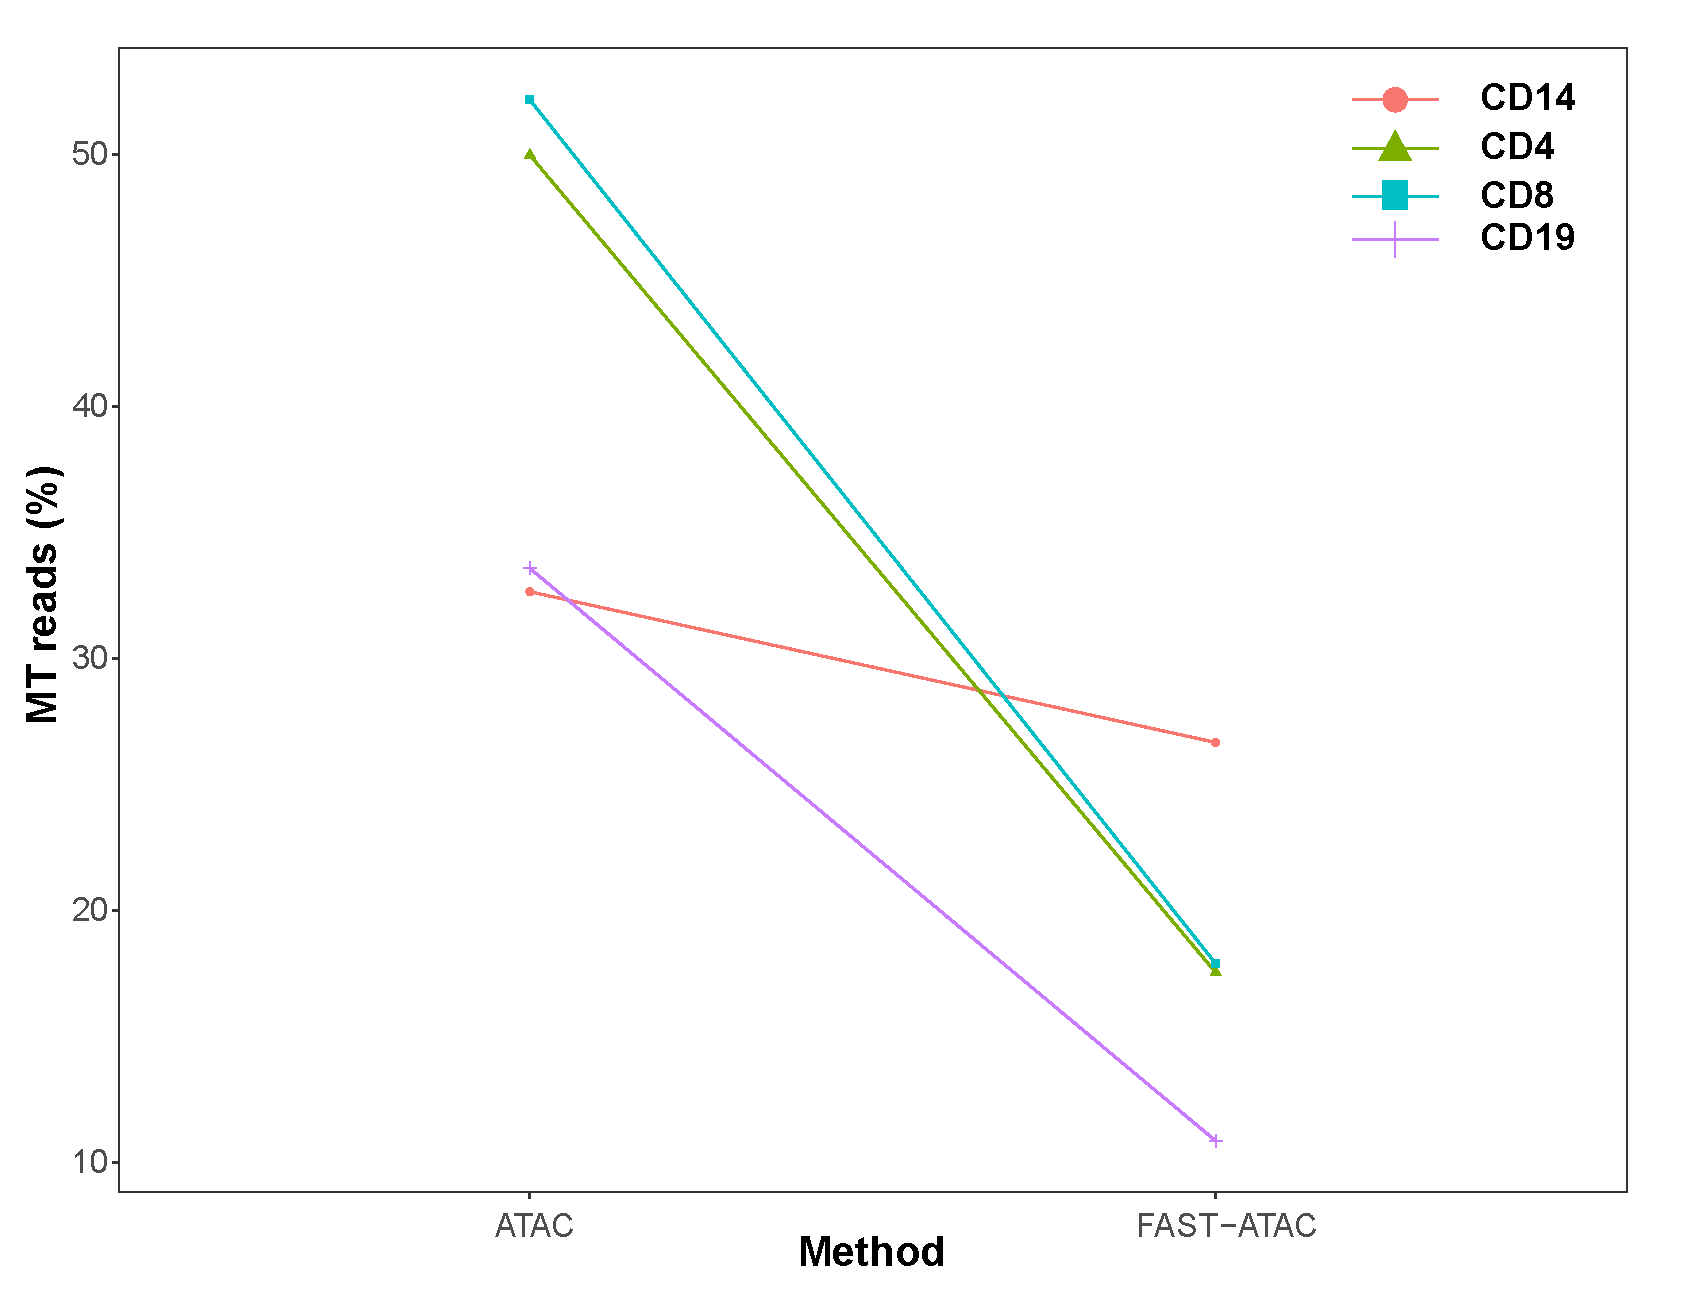
\includegraphics[width=\textwidth]{./Results1/pdfs/ATAC_vs_FAST_ATAC_percnt_MT_reads_dotplot}
\caption{\textbf{}}
% The percentage sign indicated that the other subfig goes side by side
\end{subfigure}%
\begin{subfigure}{0.5\textwidth}
\centering
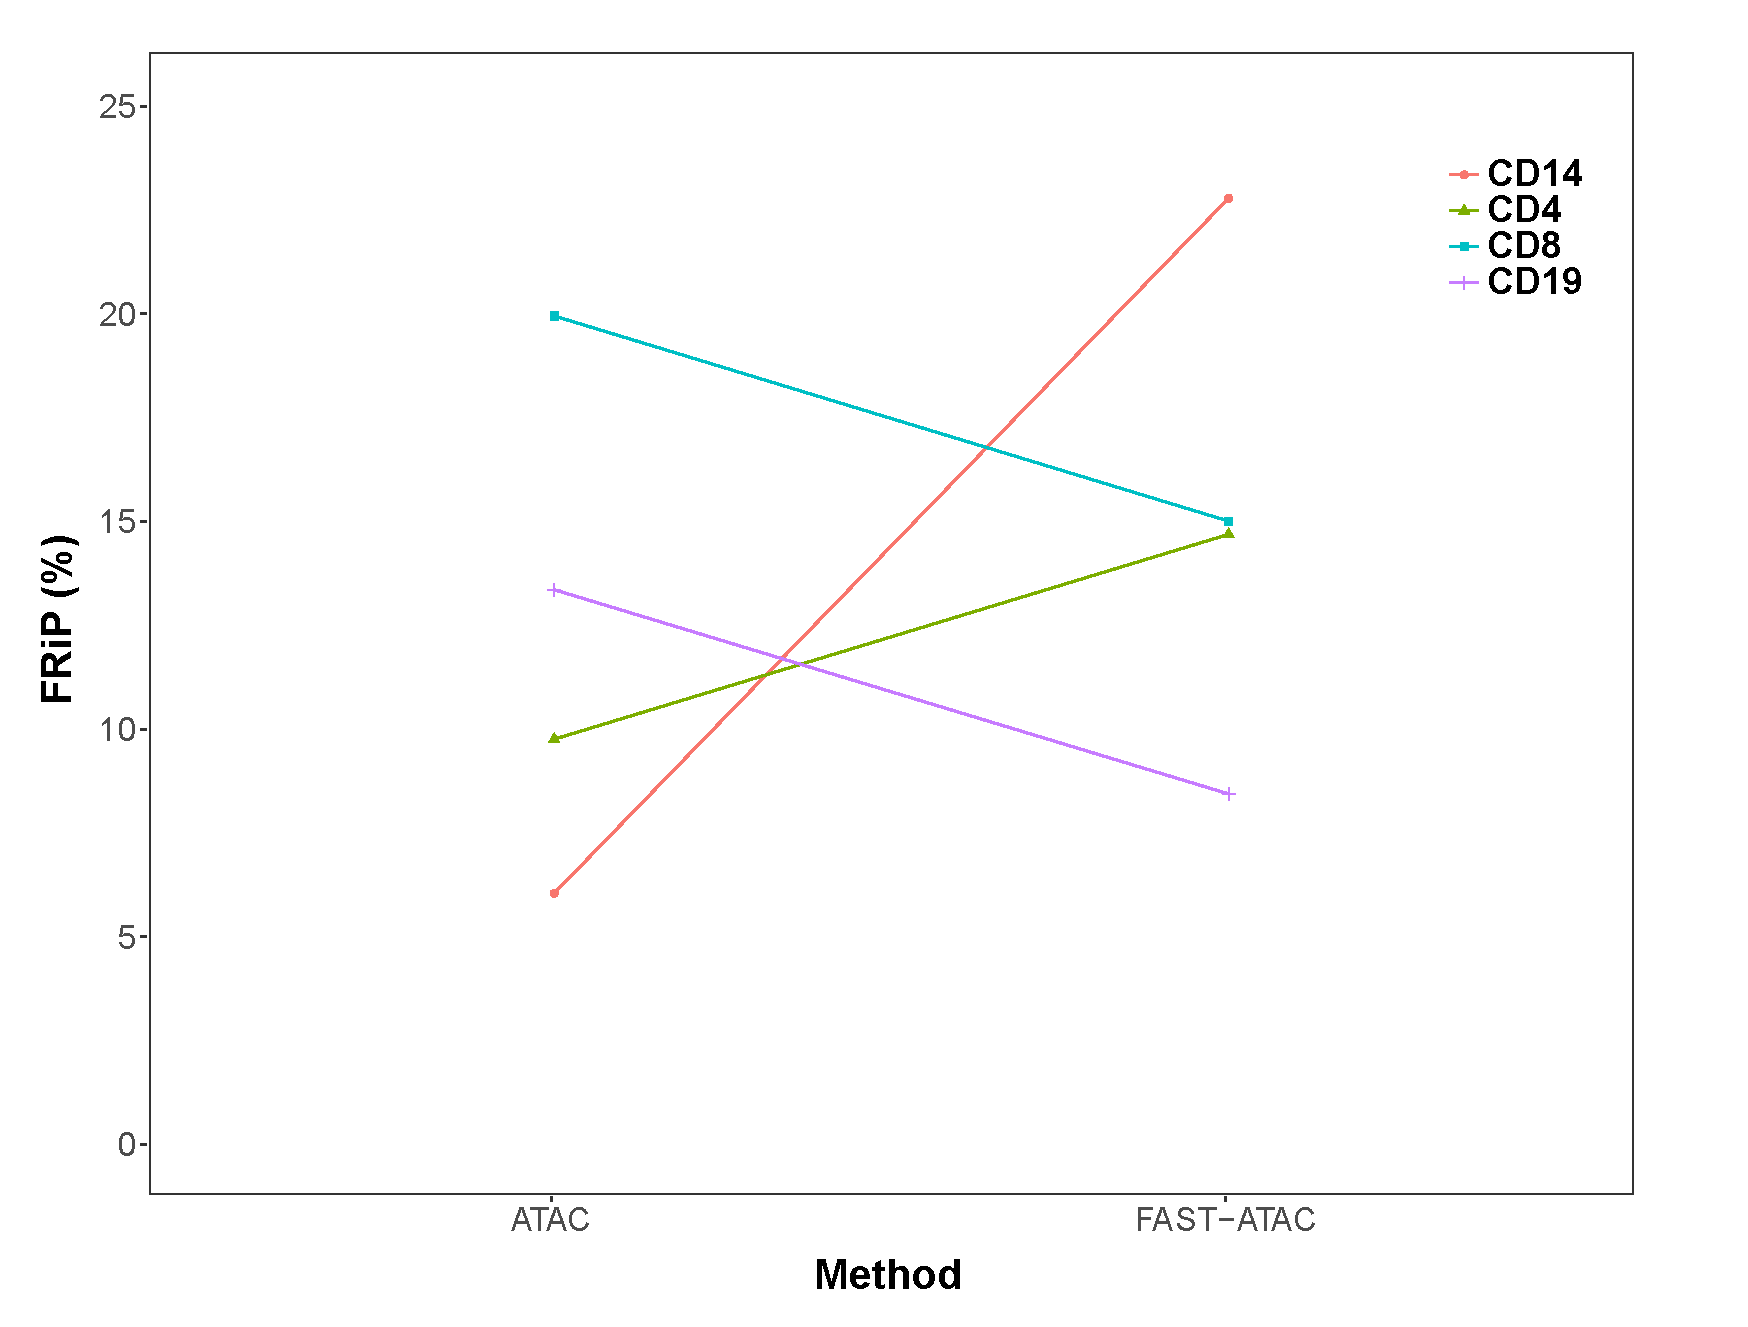
\includegraphics[width=\textwidth]{./Results1/pdfs/ATAC_vs_FAST_ATAC_FRiP_dotplot}
\caption{\textbf{}}
\end{subfigure}
\caption[Differences in MT DNA abundance and signal specificity between ATAC-seq and FAST-ATAC protocols]{\textbf{Differences in MT DNA abundance and signal specificity between ATAC-seq and FAST-ATAC protocols}}
\label{fig:ATAC_vs_FAST_ATAC}
\end{figure} 


\subsection{Impact of cryopreservation and fixation in the chromatin landscape of immune primary cells}

\subsubsection{Experimental design and cohort description}
As previously introduced, research using clinical samples represents a logistic challenge precluding immediate sample processing due to geographical and/or temporal limitations. Therefore long-term storage procedures and the use of preservatives such as fixatives facilitate handling of clinical samples. In the context of these thesis two different approaches were of interest and a collaborative project was established with High-Throughput Genomics at the Wellcome Centre for Human Genomics. On one side, the cryopreservation of PBMCs in liquid nitrogen using DMSO would allow long-term preservation and would require PBMCs thawing and recovery followed by FACS isolation of the cell population of interest. On the other hand, the use of a fixative on the FACS-isolated relevant cell types from the clinical sample could be used as a short term preservation method. Regarding fixative, there was an interest to test the performance of an optimised protocol developed by High-Throughput Genomics using DSP in scRNA-seq \parencite{}. DSP is a cell-permeable and reversible cross-linking fixative that have previously been used to preserve tissue samples for downstream immuno-staining, laser micro-dissection and RNA micro-array expression profiling \parencite{}.

In order to investigate the effect of the cryopreservation and DSP fixation in the nuclear integrity and chromatin structure, three healthy volunteers sex and age matched were processed on different days to be consistent with the case-control experimental design in psoriasis and PsA (Figure \ref{fig:Core_experimental_design}). For each of the individuals PBMCs were isolated from blood and a fraction was stained with the appropriate panel of Abs to isolate CD14$^+$ monocytes and CD4$^+$ T cells, as detailed in Chapter \label{ch:Mat}. ATAC-seq was performed directly in an aliquot of the isolated CD14$^+$ and CD4$^+$ cell. A fraction of the isolated CD14$^+$ and CD4$^+$ cell were appropriately fixed with DPS, stored at 4{$^\circ$}C for 24h and processed for ATAC-seq. A fraction of the PBMCs were cryopreserved following the protocol described in Chapter \label{ch:Mat}, stored in liquid nitrogen for approximately 1 week followed by thawing and recovery in culture for approximately 30 min before undergoing Ab staining and FACS to retrieve CD14$^+$ and CD4$^+$ cells. Altogether, for each of the three controls and two cell types three matched ATAC-seq samples were generated: ATAC-seq fresh, ATAC-seq fixed and ATAC-seq frozen.

\begin{landscape}
\begin{figure}[H]
\centering
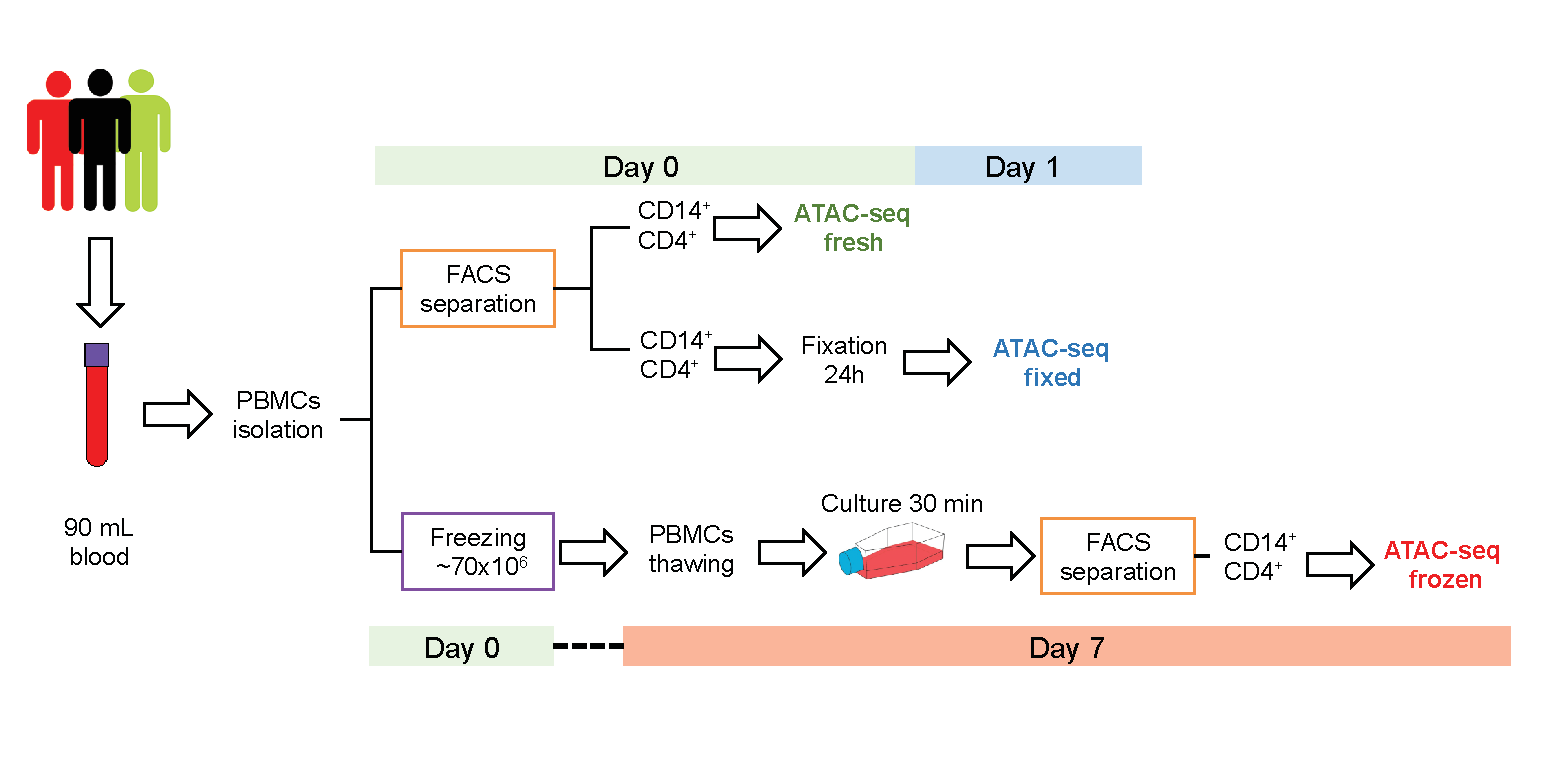
\includegraphics[width=\textwidth]{./Results1/pdfs/Chapter3_core_experimental_design}
\caption[Experimetal design to assess the impact of cryopreservation and fixation in the chromatin accessibility of immune primary cells.]{\textbf{Experimetal design to assess the impact of cryopreservation and fixation in the chromatin accessibility of immune primary cells.}}
\label{figure:Core_experimental_design}
\end{figure}
\end{landscape}



\subsubsection{Analysis of the chromatin preservation structure in the different conditions}

All samples from each of the two cell types presented more than 15 M reads, which have previously been shown as the minimum to proceed with appropriate ATAC-seq analysis (Figure \ref{figure:Core_ATAC_all_conditions_total_reads}). In the case of the CD14$^+$ monocytes the median of reads across the fresh, frozen and fixed were more similar (58.6, 64.2 and 39.6 M reads, respectively) (Figure \ref{figure:Core_ATAC_all_conditions_total_reads} a) than in the total CD4$^+$ samples, where the frozen and fixed presented lower median of total million reads compared to the controls (43.8, 32.9 and 28.8 M reads respectively)(Figure \ref{figure:Core_ATAC_all_conditions_total_reads} b).

\begin{figure}[htbp]
\centering
\begin{subfigure}{0.5\textwidth}
\centering
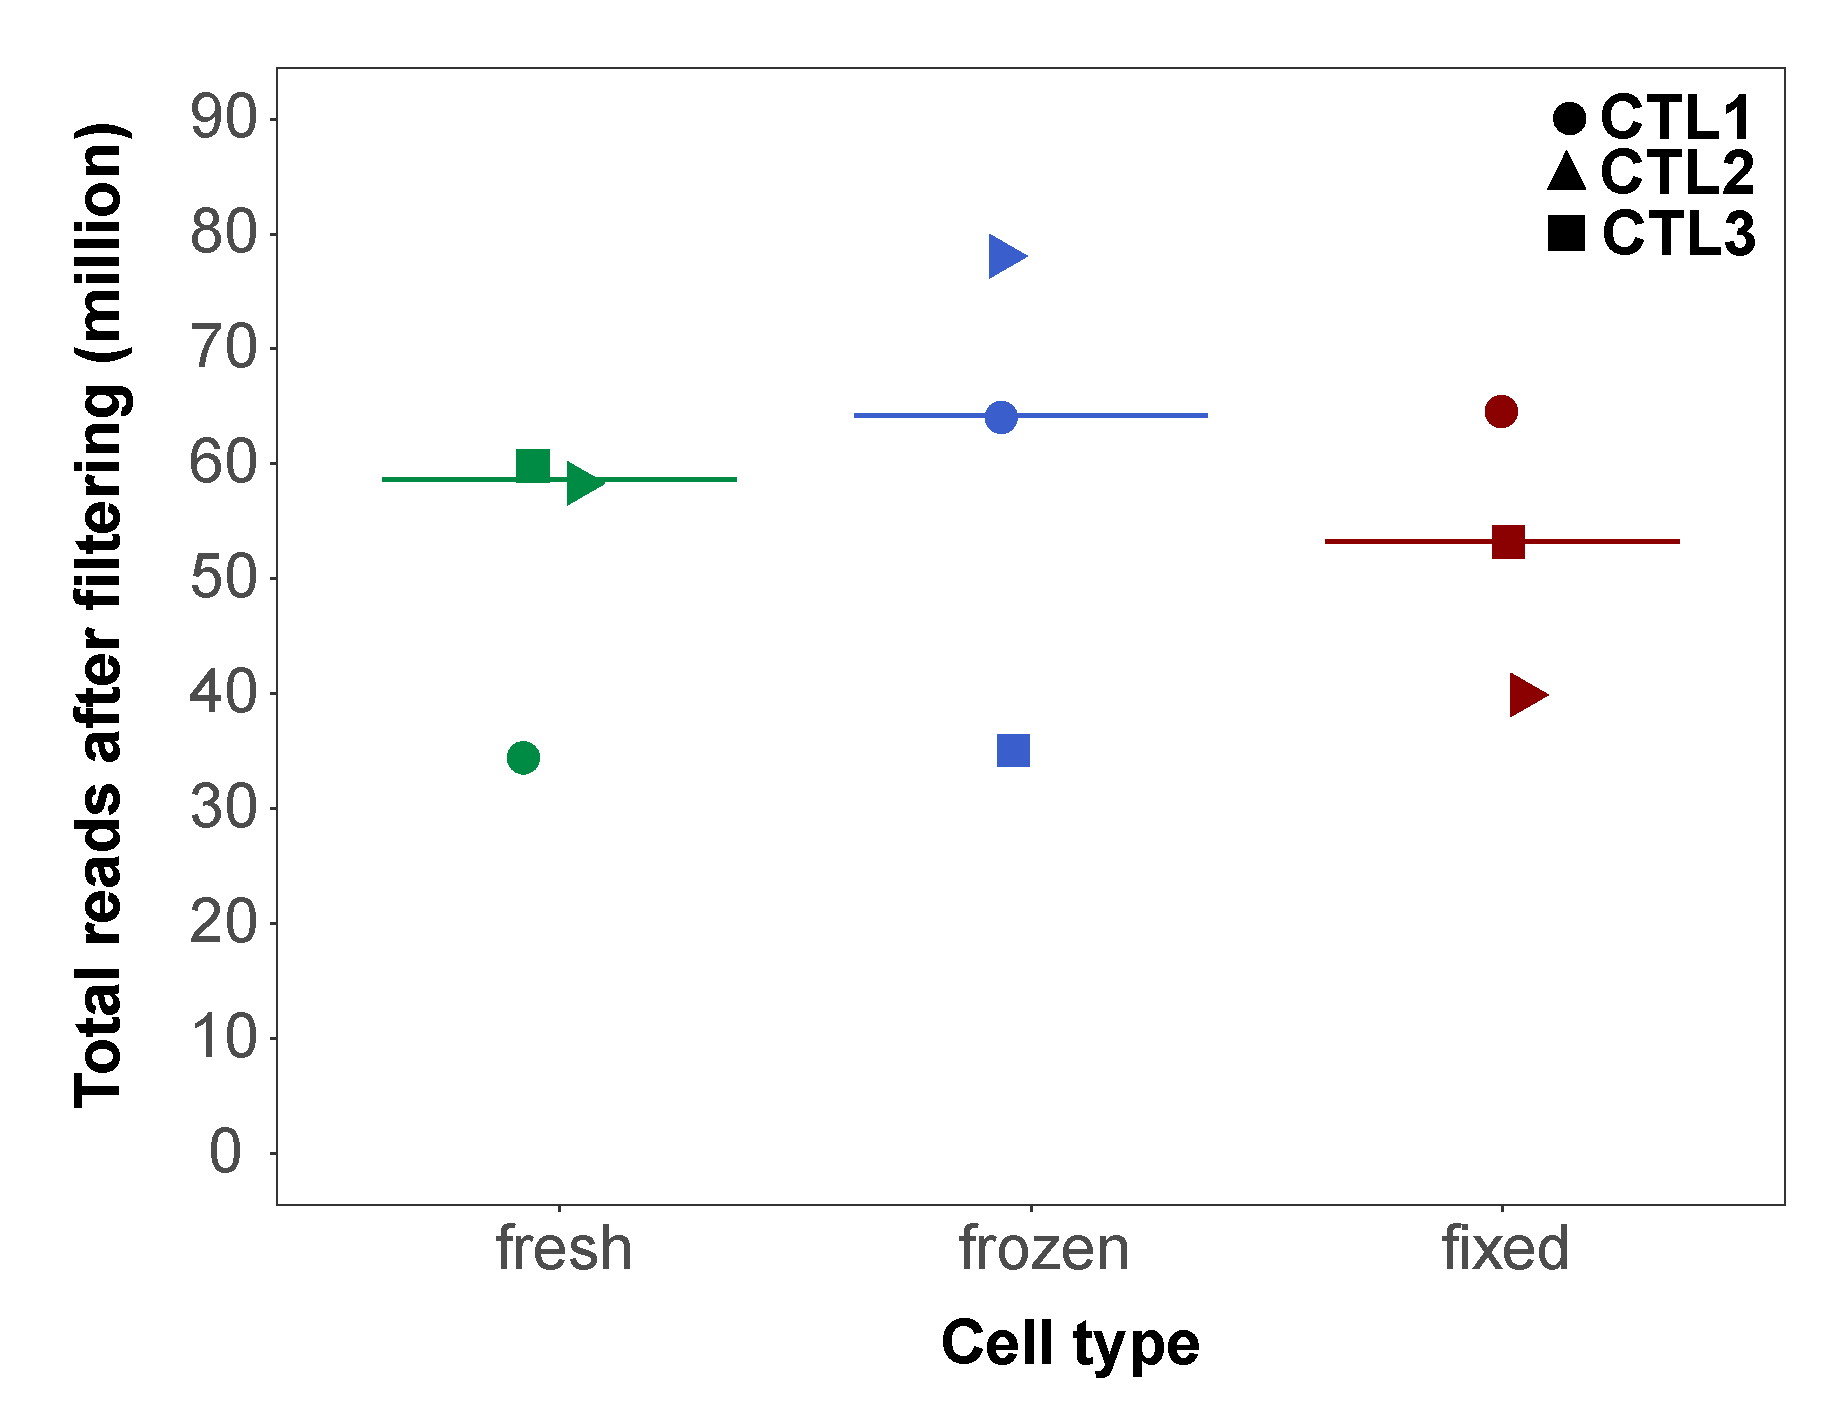
\includegraphics[width=\textwidth]{./Results1/pdfs/Core_ATAC_CD14_fresh_frozen_fixed_filtered_total_reads}
\caption{\textbf{}}
% The percentage sign indicated that the other subfig goes side by side
\end{subfigure}%
\begin{subfigure}{0.5\textwidth}
\centering
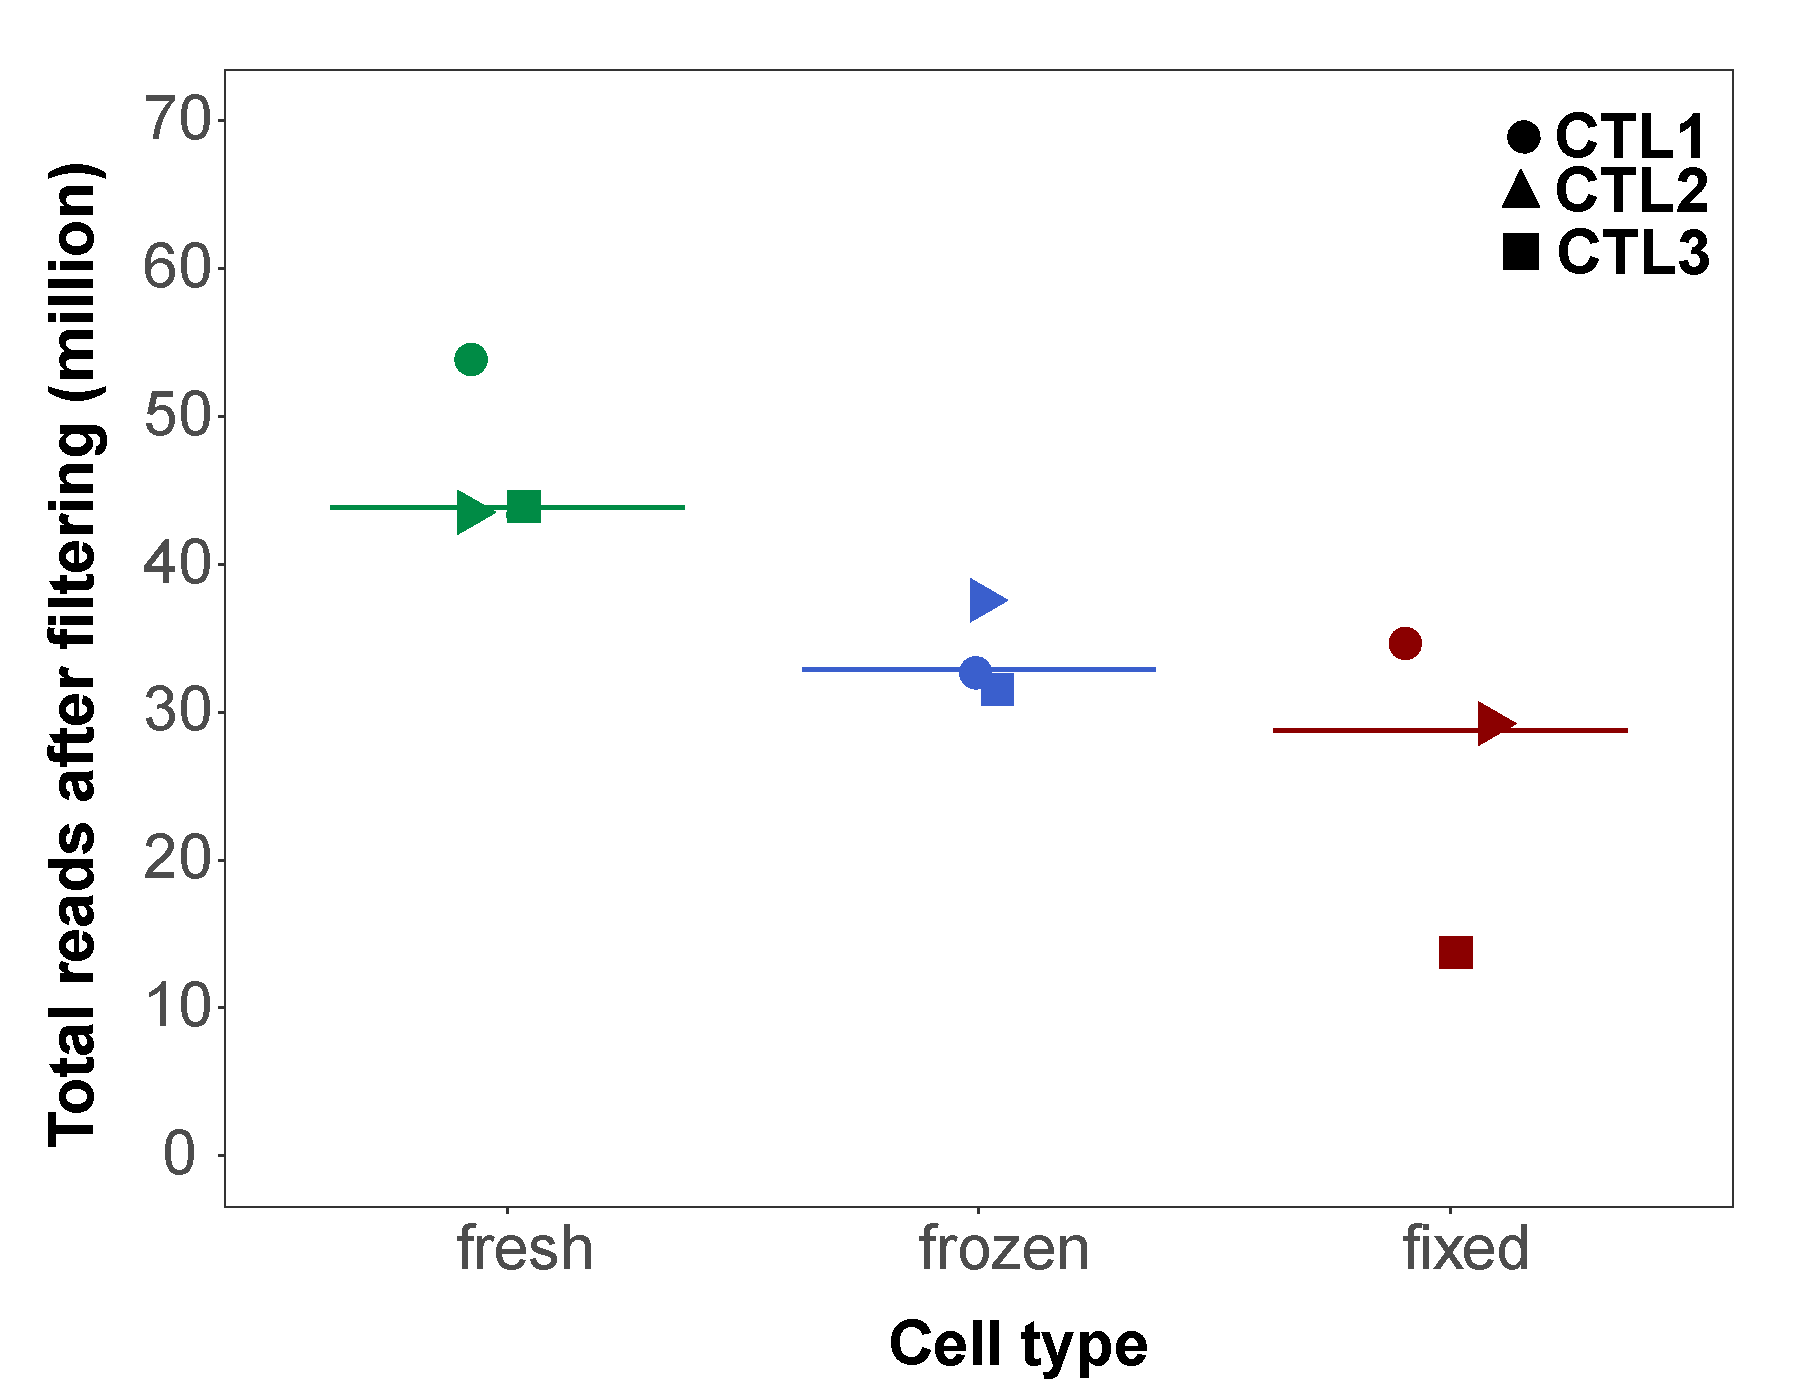
\includegraphics[width=\textwidth]{./Results1/pdfs/Core_ATAC_CD4_fresh_frozen_fixed_filtered_total_reads}
\caption{\textbf{}}
\end{subfigure}
\caption[Total number of ATAC-seq reads for the fresh, frozen and fixed CD14$^+$ monocytes and total CD4$^+$ samples.]{\textbf{Total number of ATAC-seq reads for the fresh, frozen and fixed CD14$^+$ monocytes and total CD4$^+$ samples.}}
\label{figure:Core_ATAC_all_conditions_total_reads}
\end{figure} 

The signal-to-noise ratios across the three conditions for the two cell types was quantified using enrichment of ATAC-seq reads across genes TSS. The median TSS for the CD14$^+$ monocytes was similar for the fresh and fixed libraries (17.4 and 16.5, respectively) and higher for the frozen samples(26.3)(Table \ref{tab:Core_ATAC_TSS_summary_table}). The TSS enrichments for the frozen and fixed CD4$^+$ samples (16.1 and 14.3, respectively) were considerably higher than the median of the fresh samples (5.6), which were borderline for the 6 fold-enrichmnet threhold ENCODE recommended. Interestingly, the CTL1 fixed samples of both cell types, CD14$^+$ monocytes and total CD4$^+$, presented  considerably lower TSS enrichment (2.5 and 7.9, respectively) compared to the other fixed samples (Table \ref{tab:Core_ATAC_TSS_summary_table}). 


In terms of the fragment size distribution profiles, all samples but CTL1 fixed from CD14$^+$ monocytes and total CD4$^+$, presented similar patters with a nucleosome-free fragments $<$150bp and fragments corresponding to mono-, di-, tri- and tretra-nucleosomes. Variation in the distribution across the fragments pattern were mainly observed for the fixed samples, presenting lower density of nucleosome-free fragments when compared to fresh and frozen, which were more similar between them in both cell types. CTL1 fixed in CD14$^+$ monocytes and total CD4$^+$ had extremely low abundance of nucleosome-free regions, consistently with the very low TSS enrichment for CTL1 CD14 fixed, previously highlighted. 

\begin{figure}[htbp]
\centering
\begin{subfigure}{0.5\textwidth}
\centering
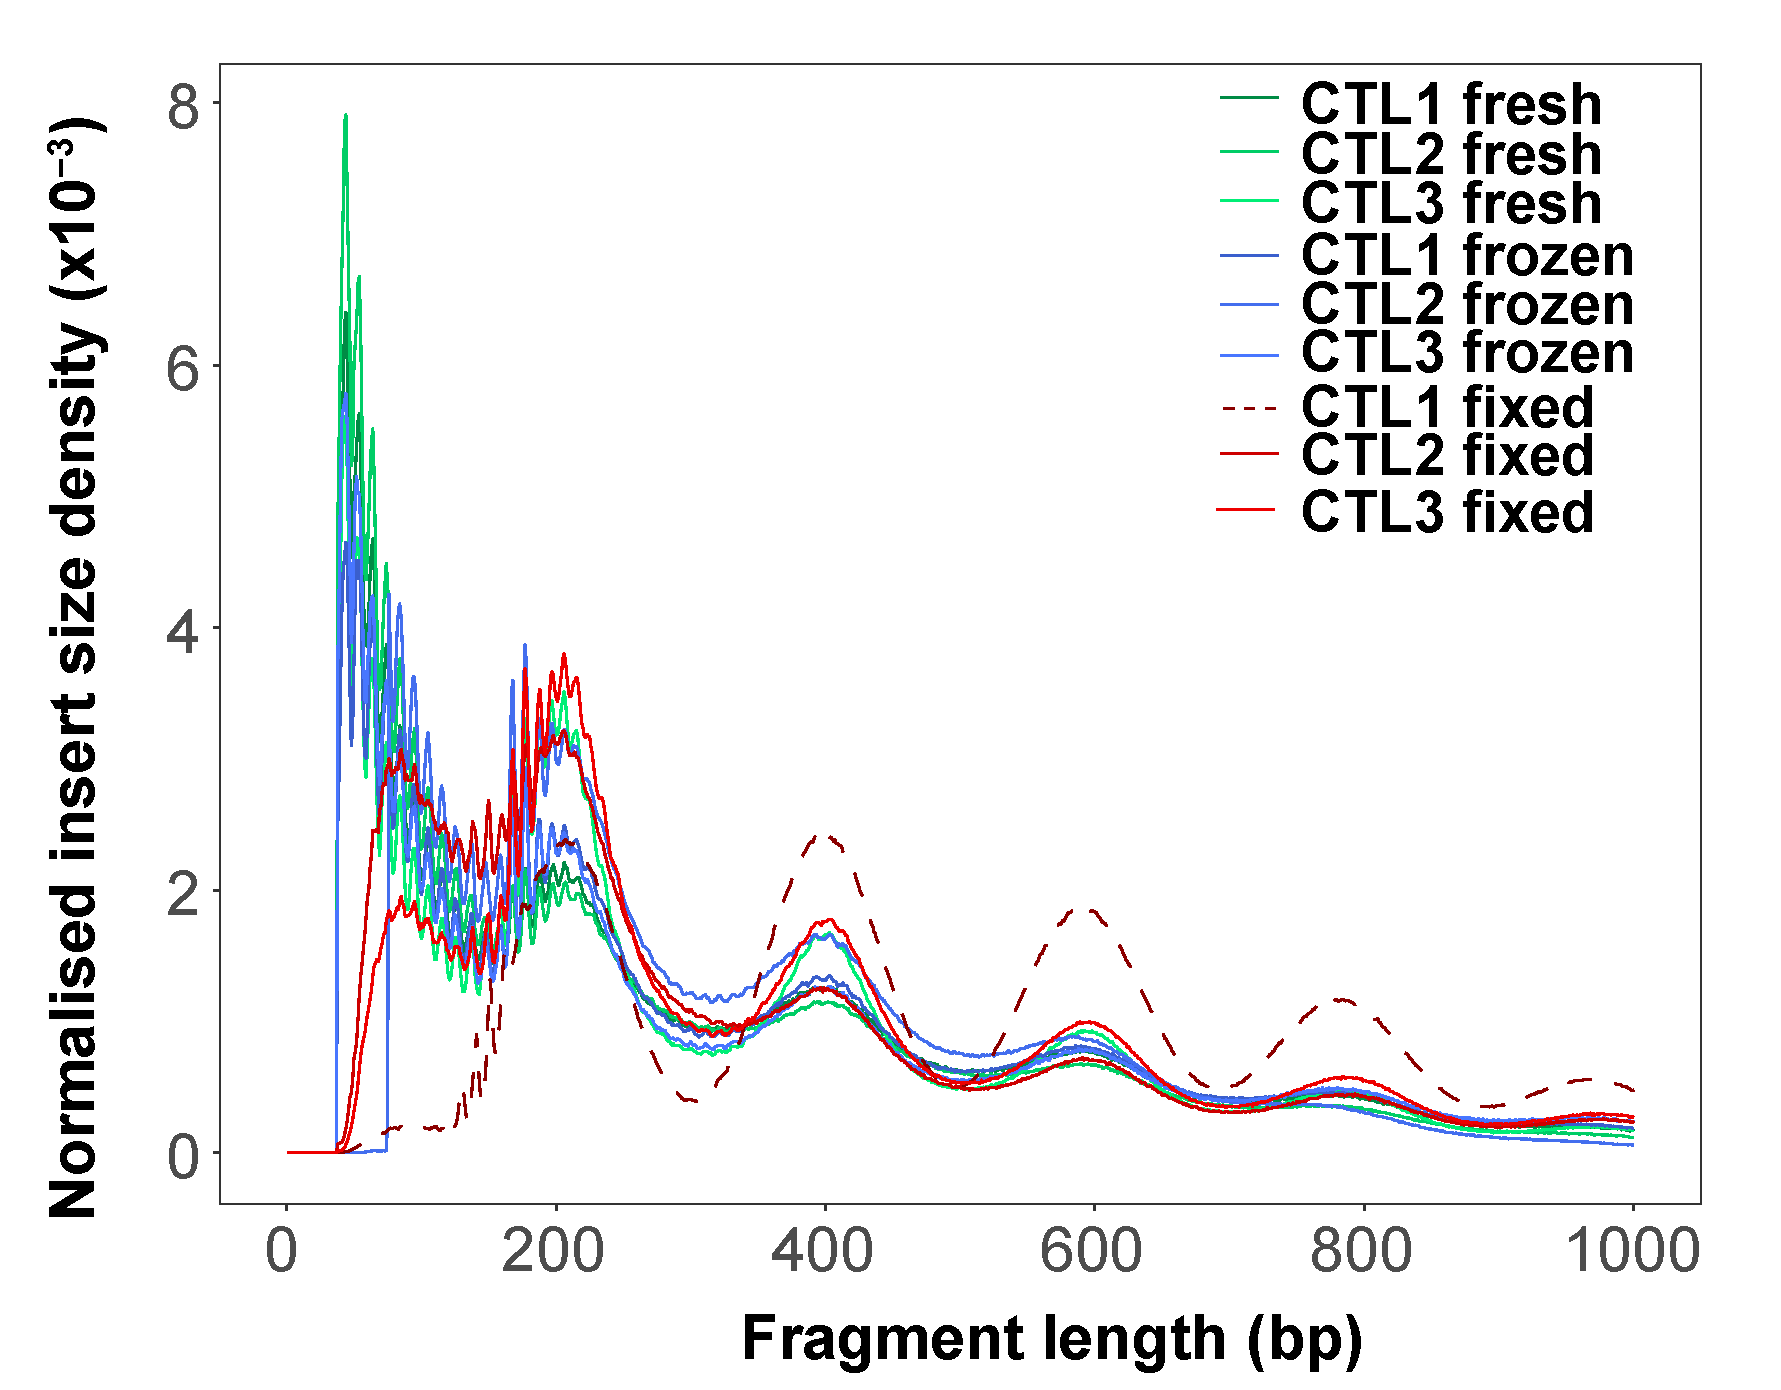
\includegraphics[width=\textwidth]{./Results1/pdfs/Core_ATAC_CD14_fresh_frozen_fixed_frag_size_distribution}
\caption{\textbf{}}
% The percentage sign indicated that the other subfig goes side by side
\end{subfigure}%
\begin{subfigure}{0.5\textwidth}
\centering
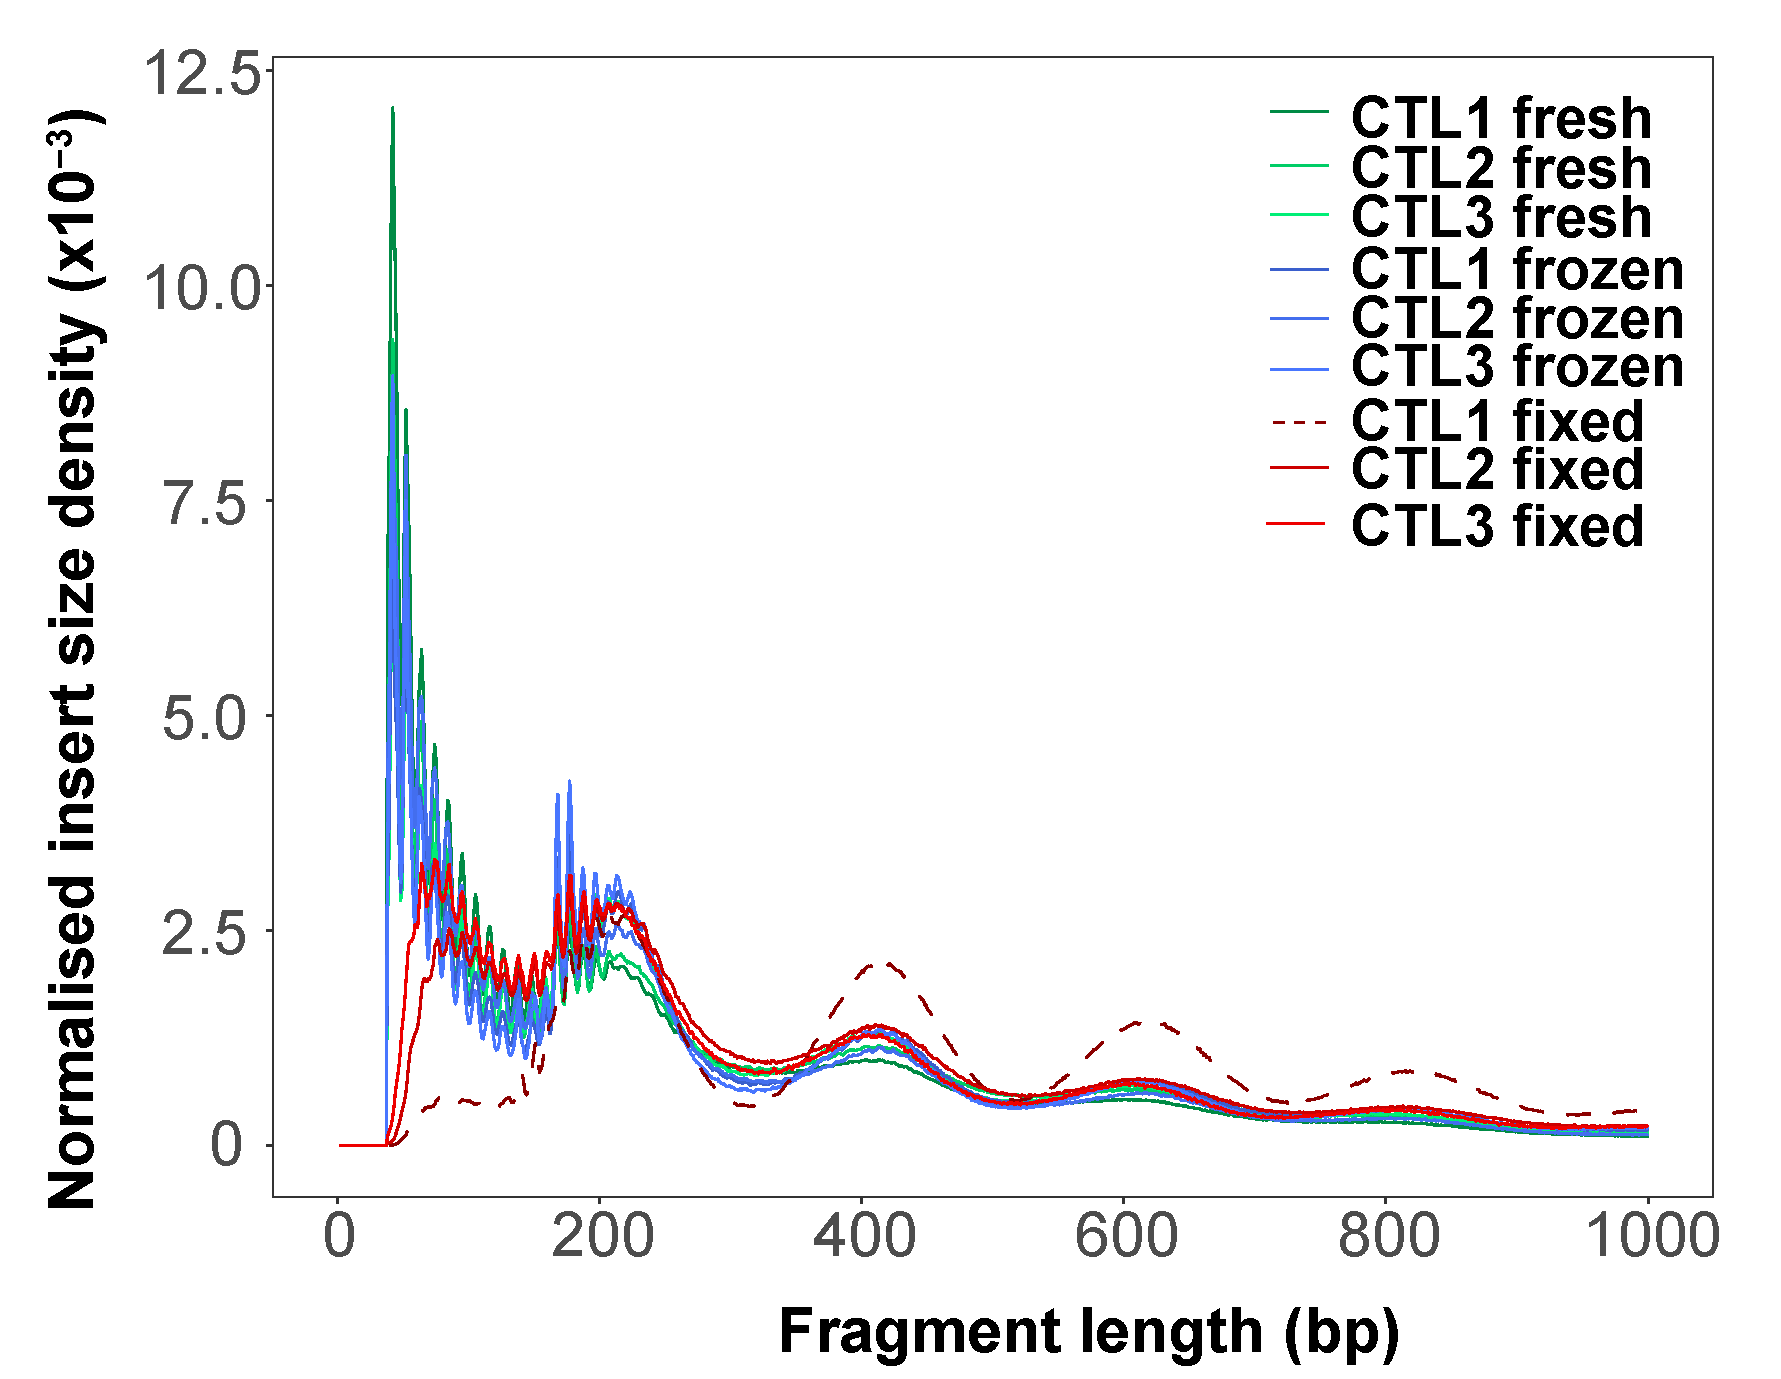
\includegraphics[width=\textwidth]{./Results1/pdfs/Core_ATAC_CD4_fresh_frozen_fixed_frag_size_distribution}
\caption{\textbf{}}
\end{subfigure}
\caption[Total number of ATAC-seq reads for the fresh, frozen and fixed CD14$^+$ monocytes and total CD4$^+$ samples.]{\textbf{Total number of ATAC-seq reads for the fresh, frozen and fixed CD14$^+$ monocytes and total CD4$^+$ samples.}}
\label{figure:Core_ATAC_all_conditions_total_reads}
\end{figure} 




This preservation of the typical ATAC-seq fragment size distribution was also consistent with the maintenance of chromatin structure within the TSS and their surroundings. The nucleosome-free fragments from all the samples showed to be enriched within the TSS, presenting the lowest enrichment the CD4$^+$ fresh samples (Figure \ref{figure:Core_ATAC_intra_dinucleosome_tss_enrichment} a and c). The enrichment of di-nucleosome fragments (between 260 and 340bp) in the TSS surroundings showed the characteristic periodicity of the upstream and downstream positioned nucleosomes in all the samples but in the CTL1 CD14$^+$ fixed (Figure \ref{figure:Core_ATAC_intra_dinucleosome_tss_enrichment} b and d). This patters was also weaker for the three fresh samples from CD4$^+$. Interestingly, this analysis demonstrated that the overall low sample quality for the CTL1 CD14 fixed sample is dominated by the low signal-to-noise ratio from the most abundant fragments (di-, tri- and tretra-nucleosomes) driving the loss of chromatin structure in the TSS surroundings. Conversely, the fresh CD4$^+$ samples presented low enrichment for the nucleosome-free fragments in the TSS, recapitulating their overall TSS enrichment (Table \ref{tab:Core_ATAC_TSS_summary_table}) and still recapitulated weakly the two nucleosome positioned in the TSS surroundings. Altogether, freezing and, importantly fixing, appeared to maintain overall the chromatin structure, with some particular outliers exceptions, particularly CTL1 fixed CD14.

\begin{figure}[H]
\centering
\begin{subfigure}[b]{0.45\textwidth}
\centering 
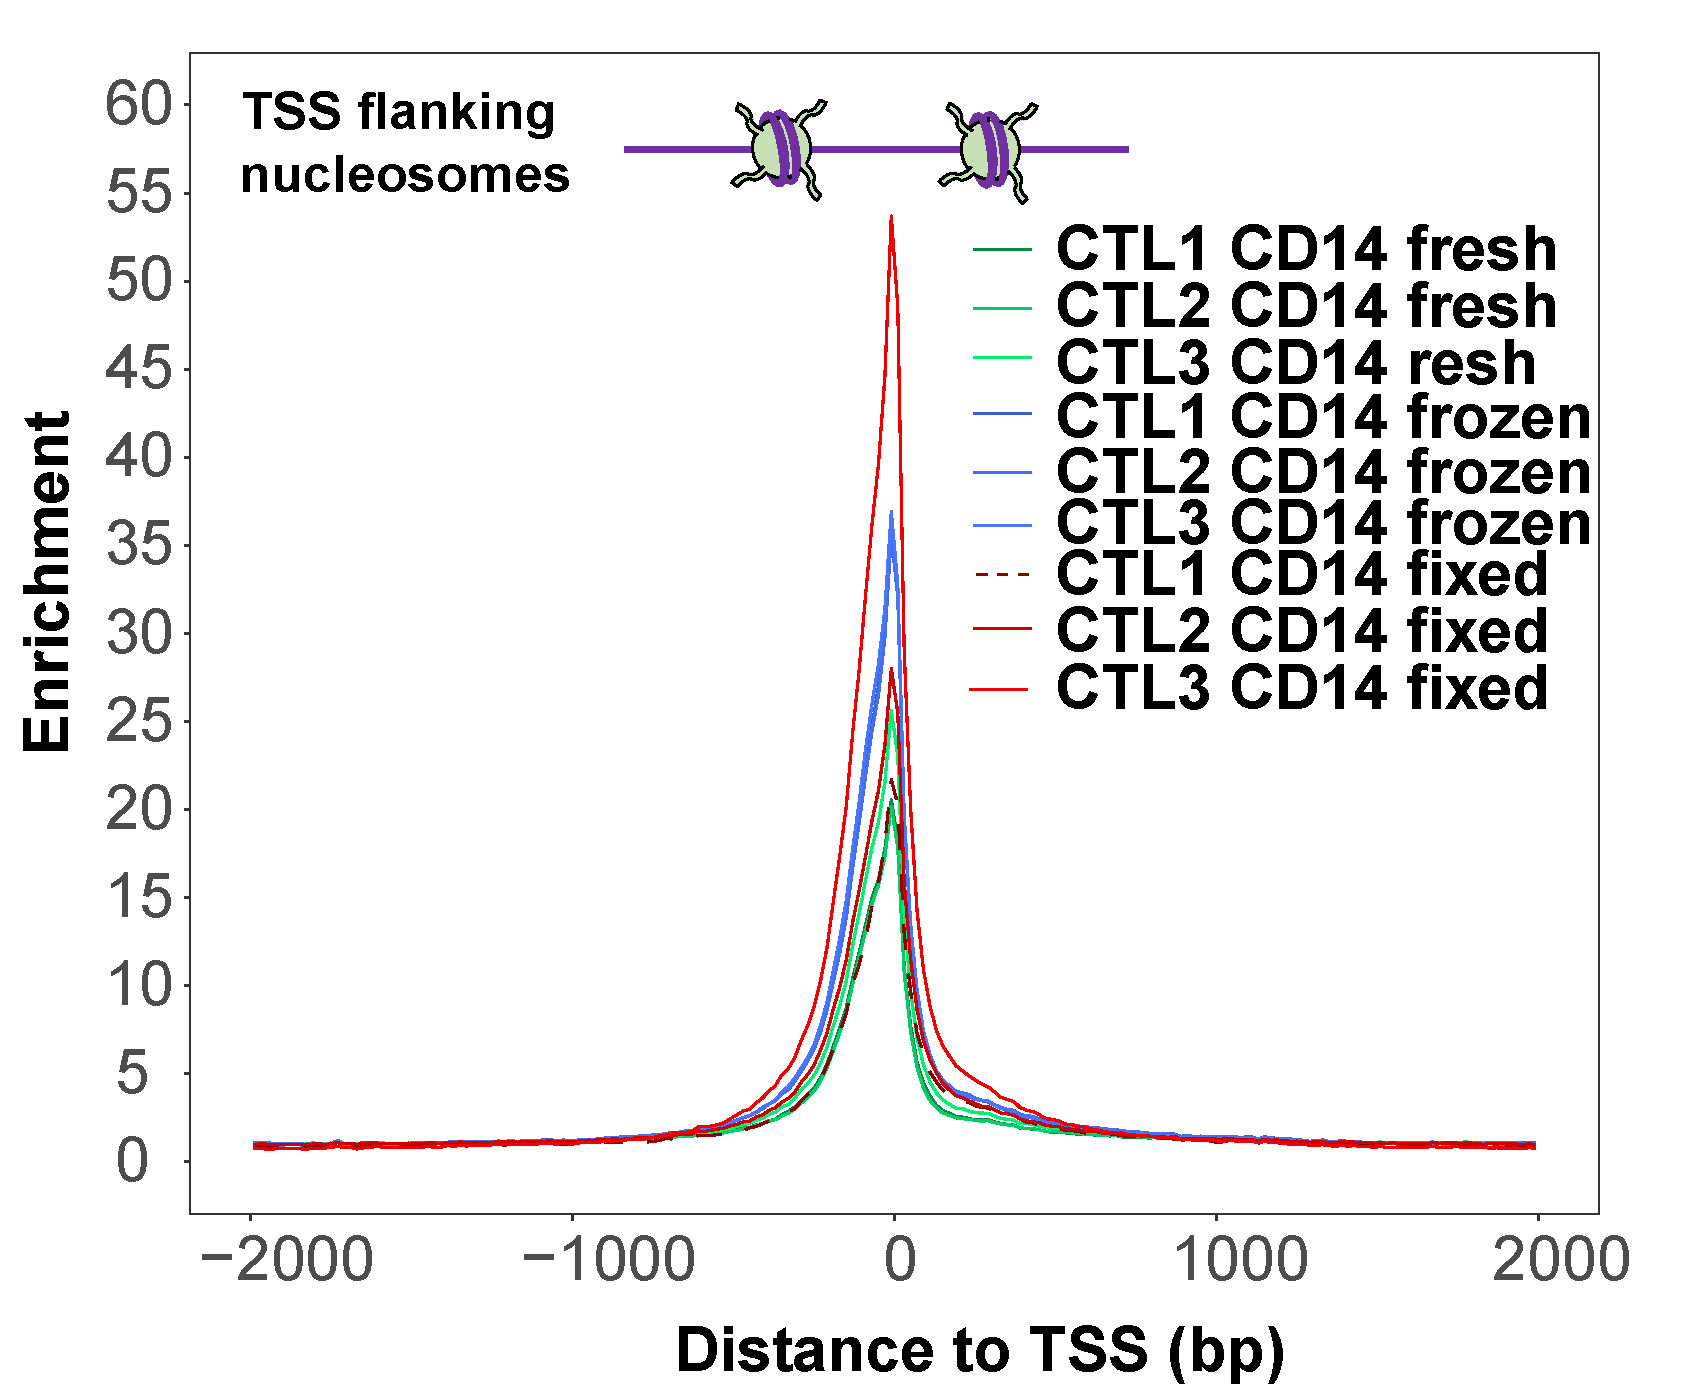
\includegraphics[width=\textwidth]{./Results1/pdfs/Core_ATAC_CD14_fresh_frozen_fixed_internucleosome_TSS}
\caption{}
\end{subfigure}
~
\begin{subfigure}[b]{0.45\textwidth}
\centering 
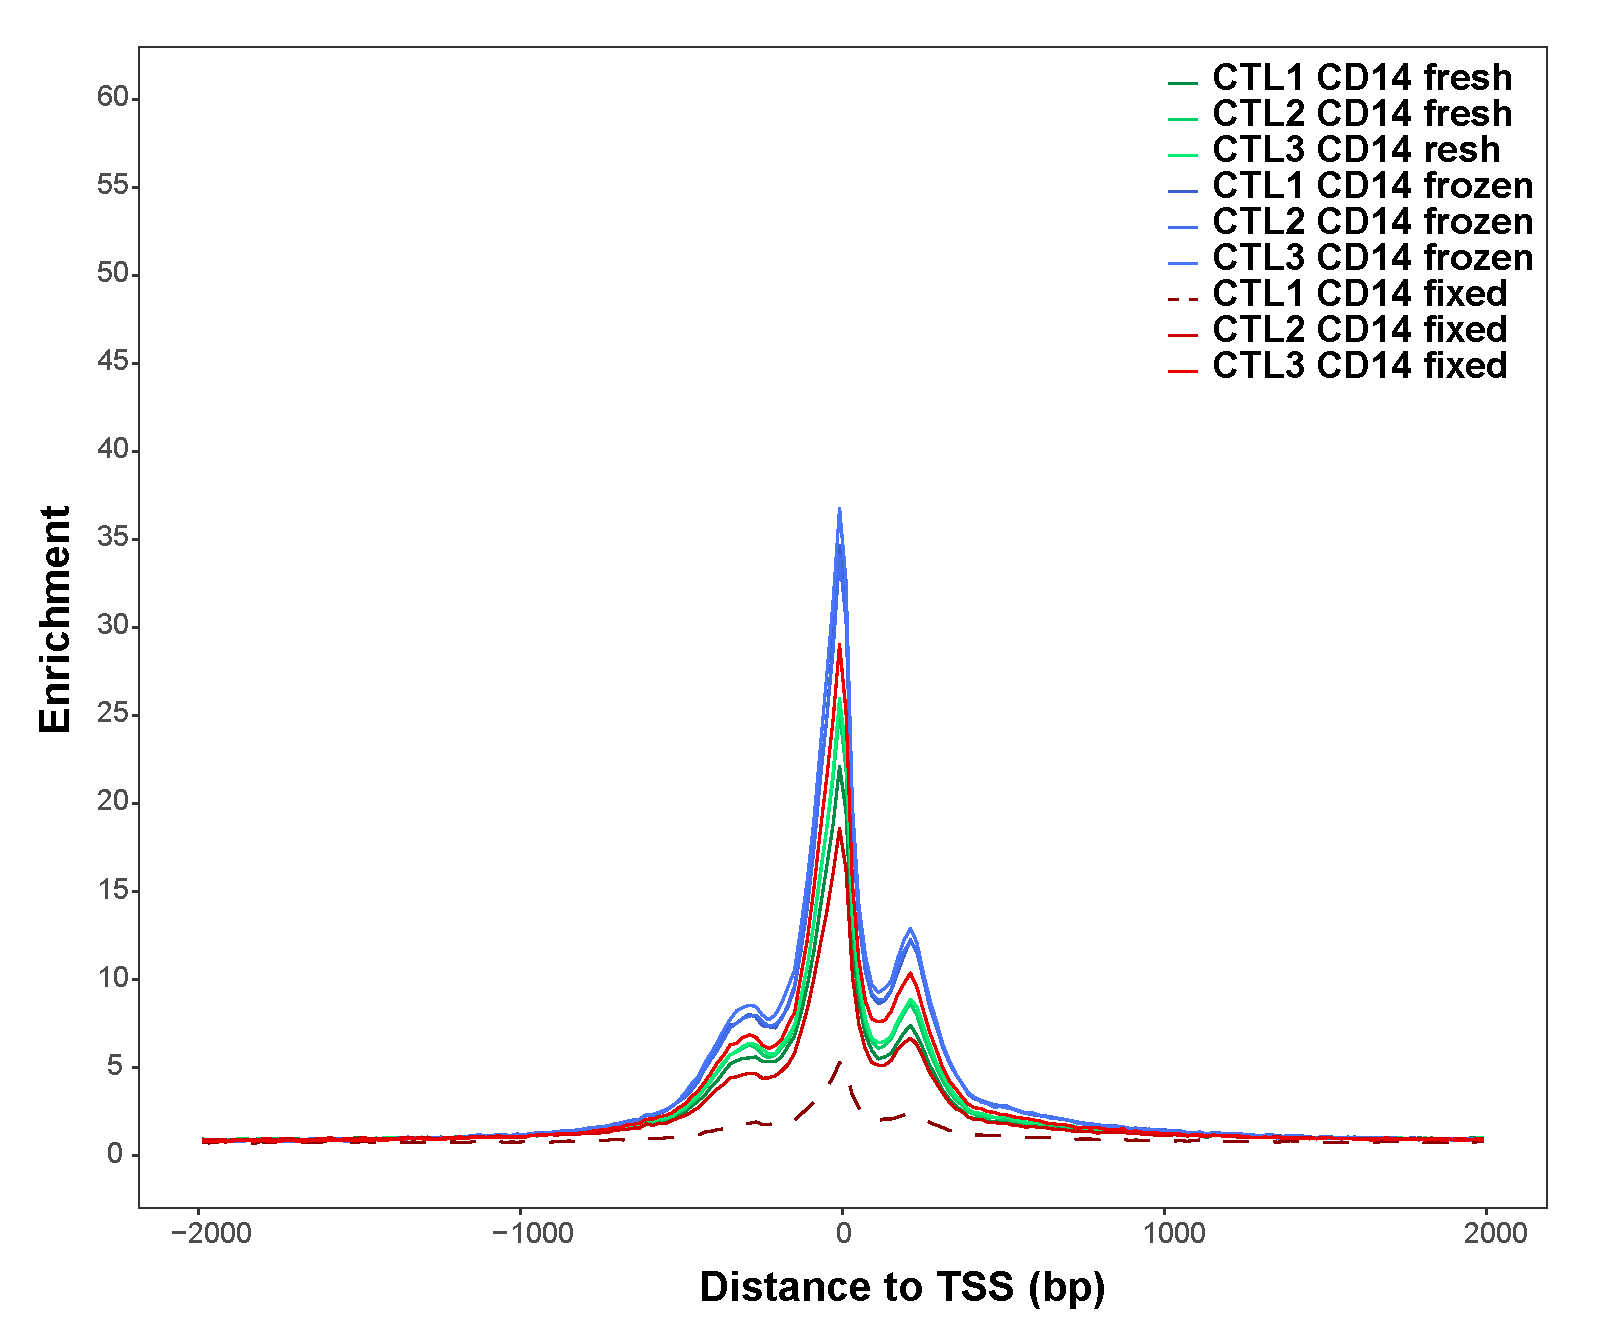
\includegraphics[width=\textwidth]{./Results1/pdfs/Core_ATAC_CD14_fresh_frozen_fixed_dinucleosome_TSS}
\caption{}
\end{subfigure}
~
\begin{subfigure}[b]{0.45\textwidth} 
%the [b] prevents offset in subcaptions
\centering
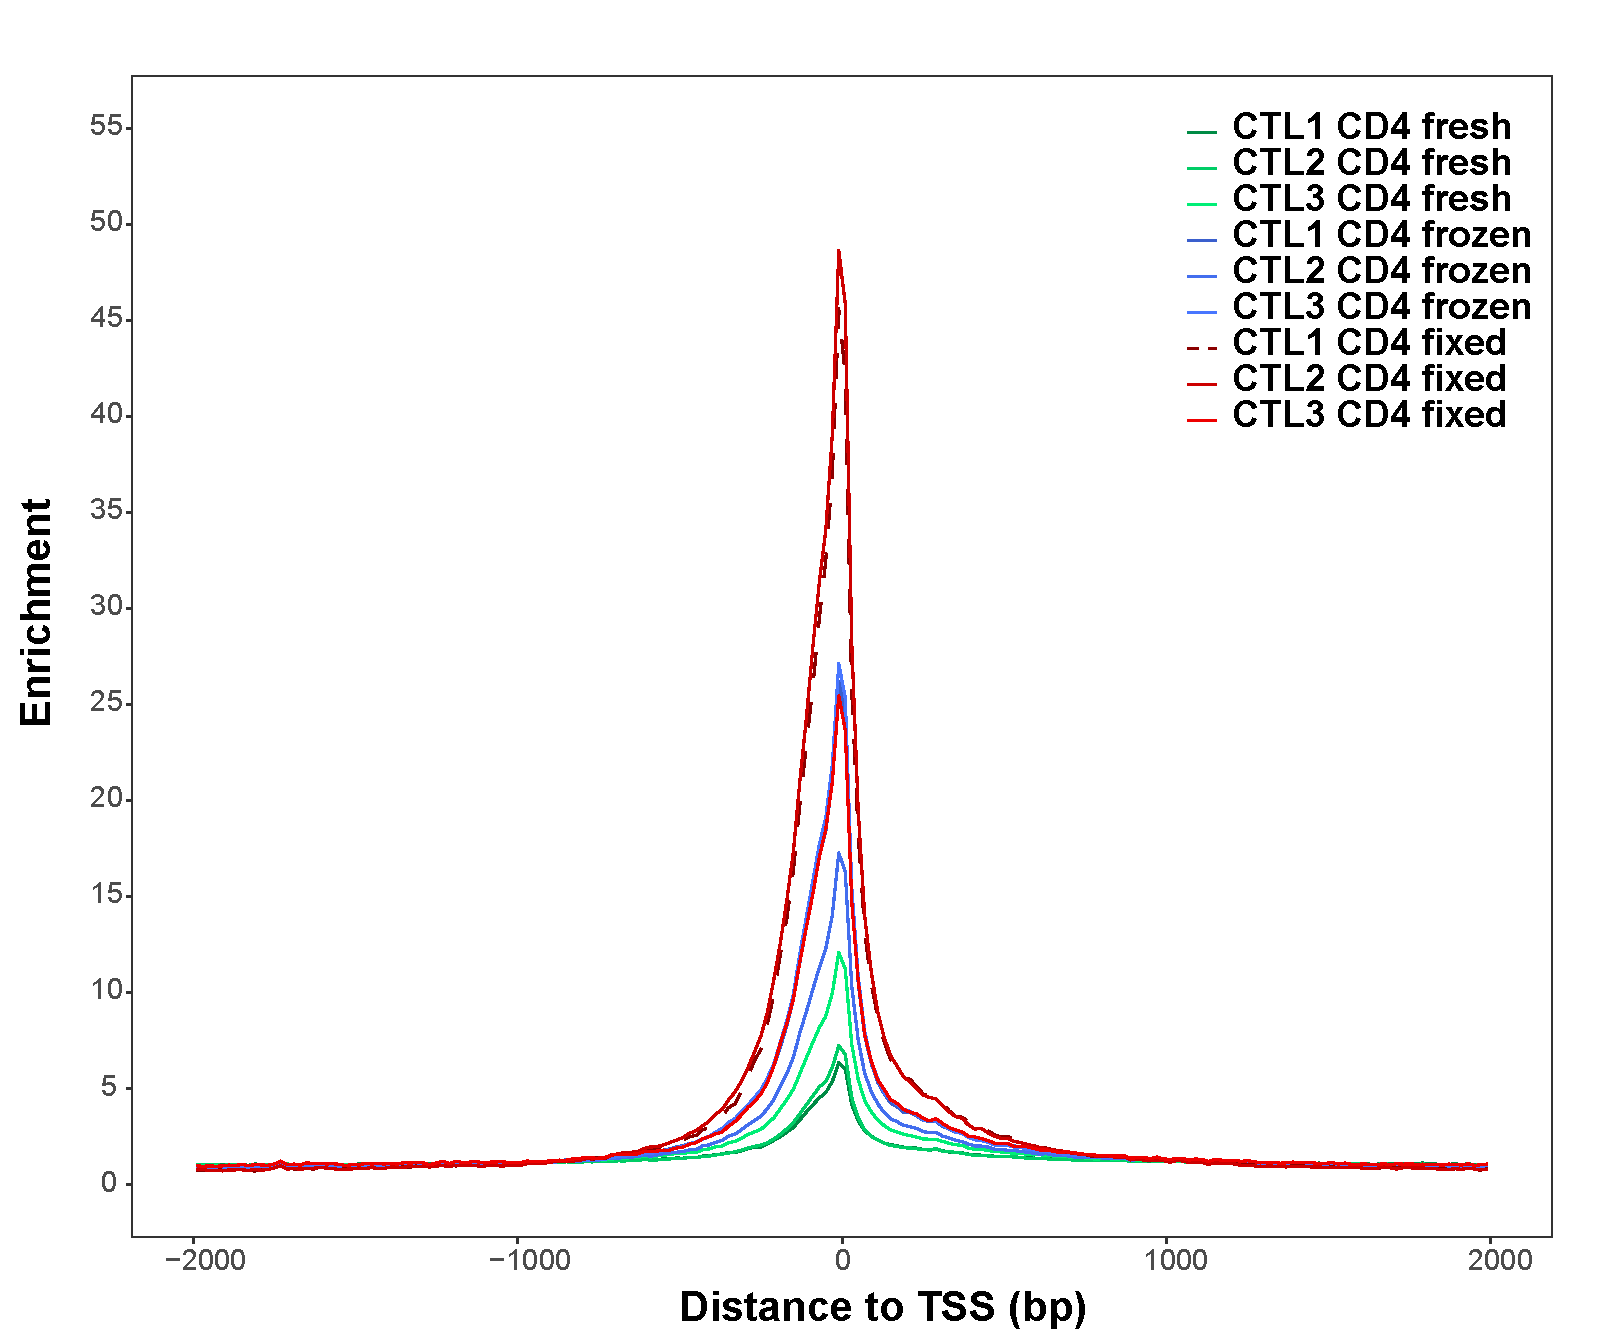
\includegraphics[width=\textwidth]{./Results1/pdfs/Core_ATAC_CD4_fresh_frozen_fixed_internucleosome_TSS}%
\caption{}
\end{subfigure}
\begin{subfigure}[b]{0.45\textwidth} 
%the [b] prevents offset in subcaptions
\centering
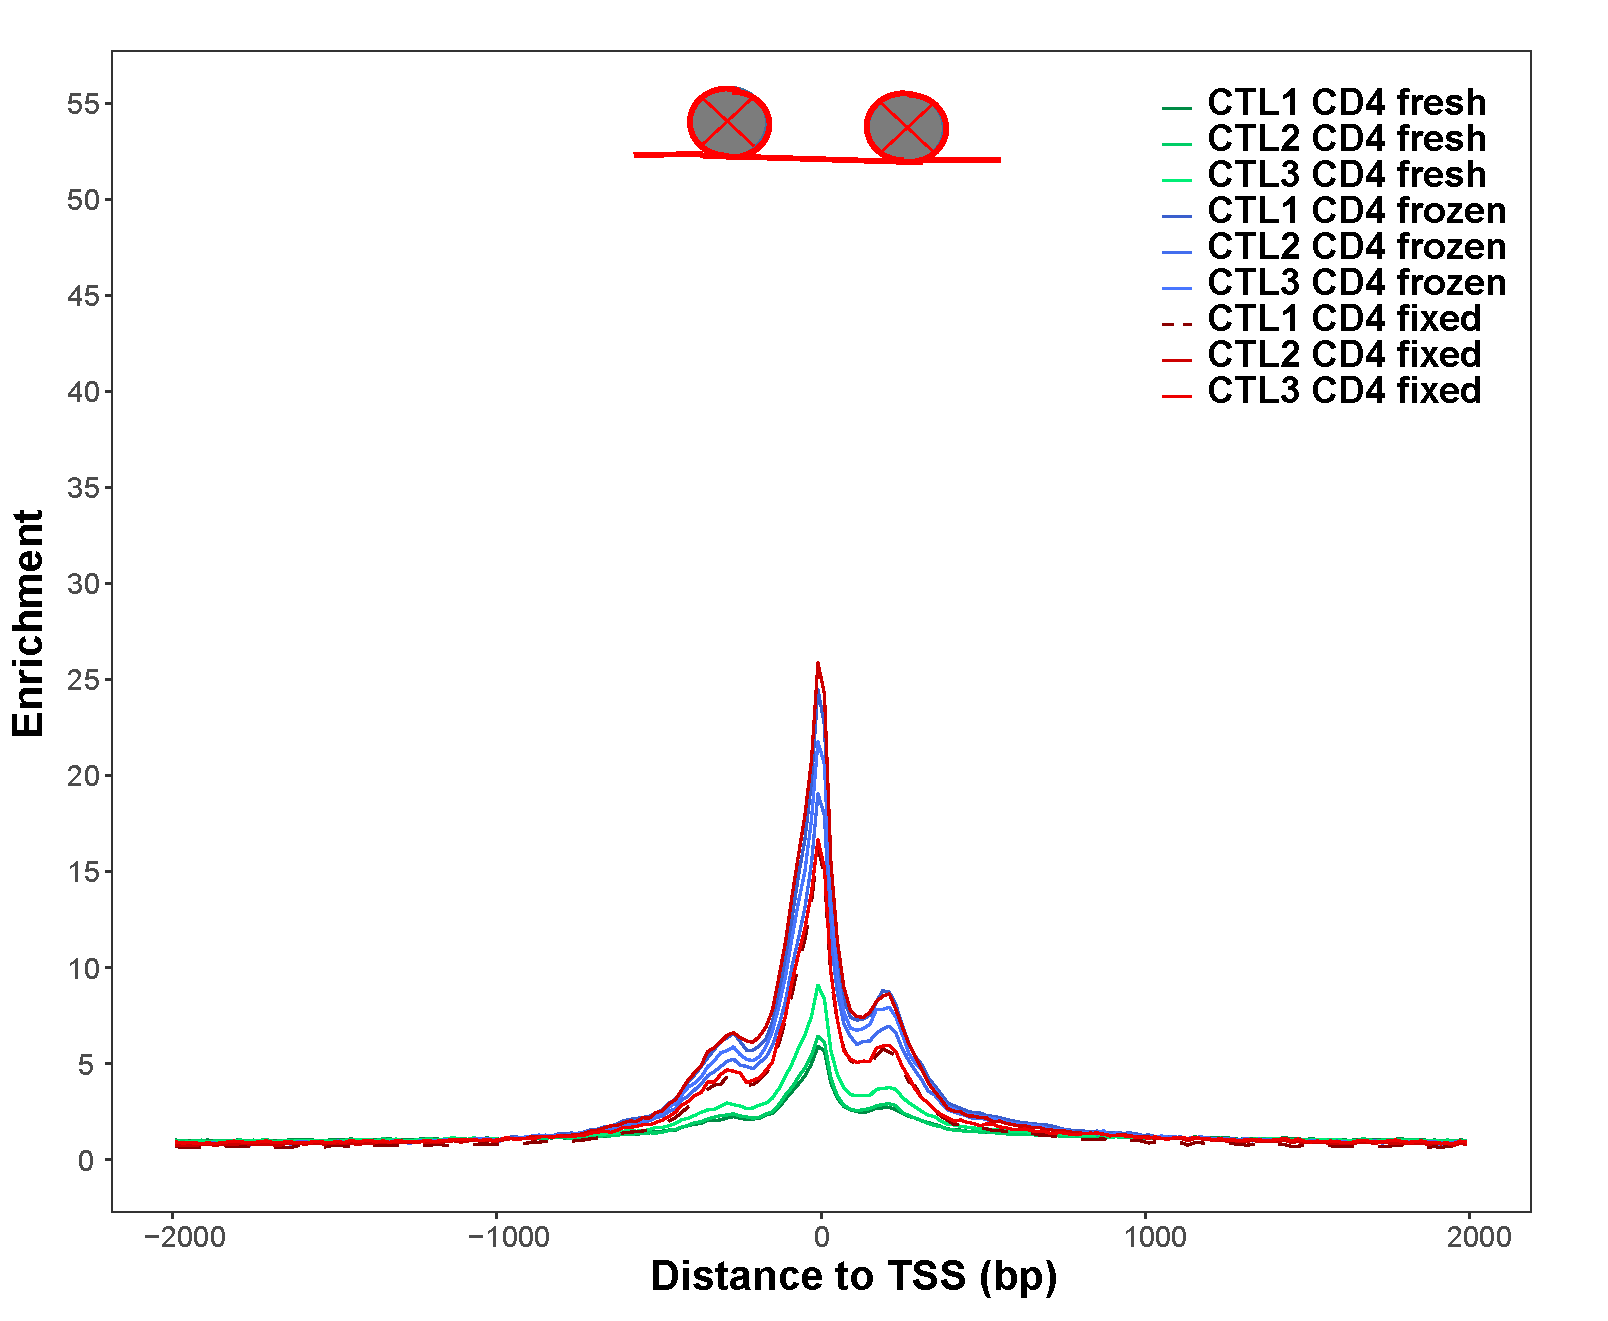
\includegraphics[width=\textwidth]{./Results1/pdfs/Core_ATAC_CD4_fresh_frozen_fixed_dinucleosome_TSS}%
\caption{}
\end{subfigure}
\caption[ATAC-seq enrichment of nucleosome-free and di-nucleosome fragments at the TSS and surroundings in CD14$^+$ monocytes and total CD4$^+$ samples for the three conditions.]{ATAC-seq enrichment of nucleosome-free and di-nucleosome fragments at the TSS and surroundings in CD14$^+$ monocytes and total CD4$^+$ samples for the three conditions.} Nucleosome-free fragments ($<$150bp) and di-nucleosome (between 260 and 340bp) were selected \textit{in silico} followed by enrichment analysis +/-1KB across all the Ensembl TSS.}
\label{figure:Core_ATAC_intra_dinucleosome_tss_enrichment}
\end{figure}





Regarding annotation, called peaks filtered for FDR$<$0.01 from all libraries for the three conditions and two cell types successfully recapitulated the distribution across different genomic features previously shown in the literature, being the greatest percentage of ATAC-seq peaks located at promoters, introns and intergenic regions (ref). Overall this suggested that freezing or fixing did not biased that distribution (Figure \ref{figure:Core_ATAC_all_conditions_genomic_features} a and b).  
 
\begin{figure}[htbp]
\centering
\begin{subfigure}{0.5\textwidth}
\centering
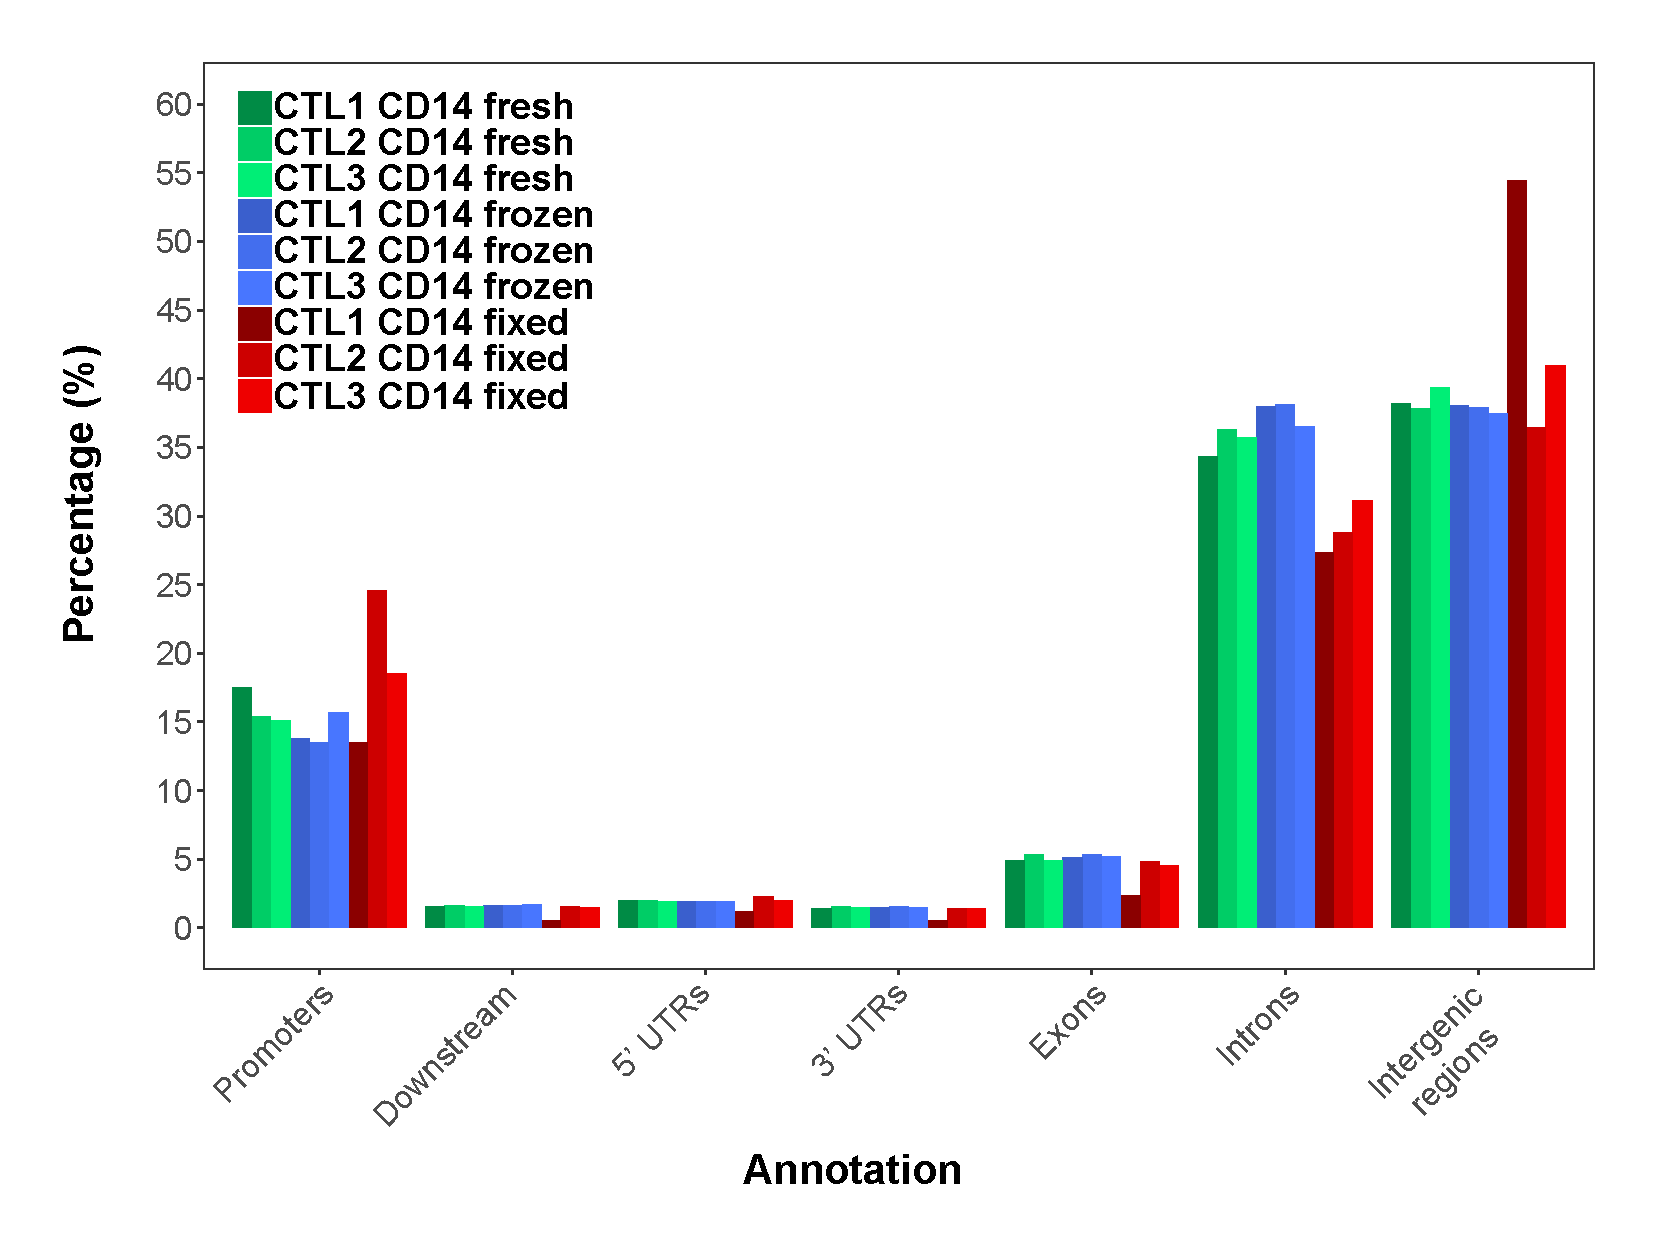
\includegraphics[width=\textwidth]{./Results1/pdfs/Core_ATAC_CD14_fresh_frozen_fixed_general_peak_annotation}
\caption{\textbf{}}
% The percentage sign indicated that the other subfig goes side by side
\end{subfigure}%
\begin{subfigure}{0.5\textwidth}
\centering
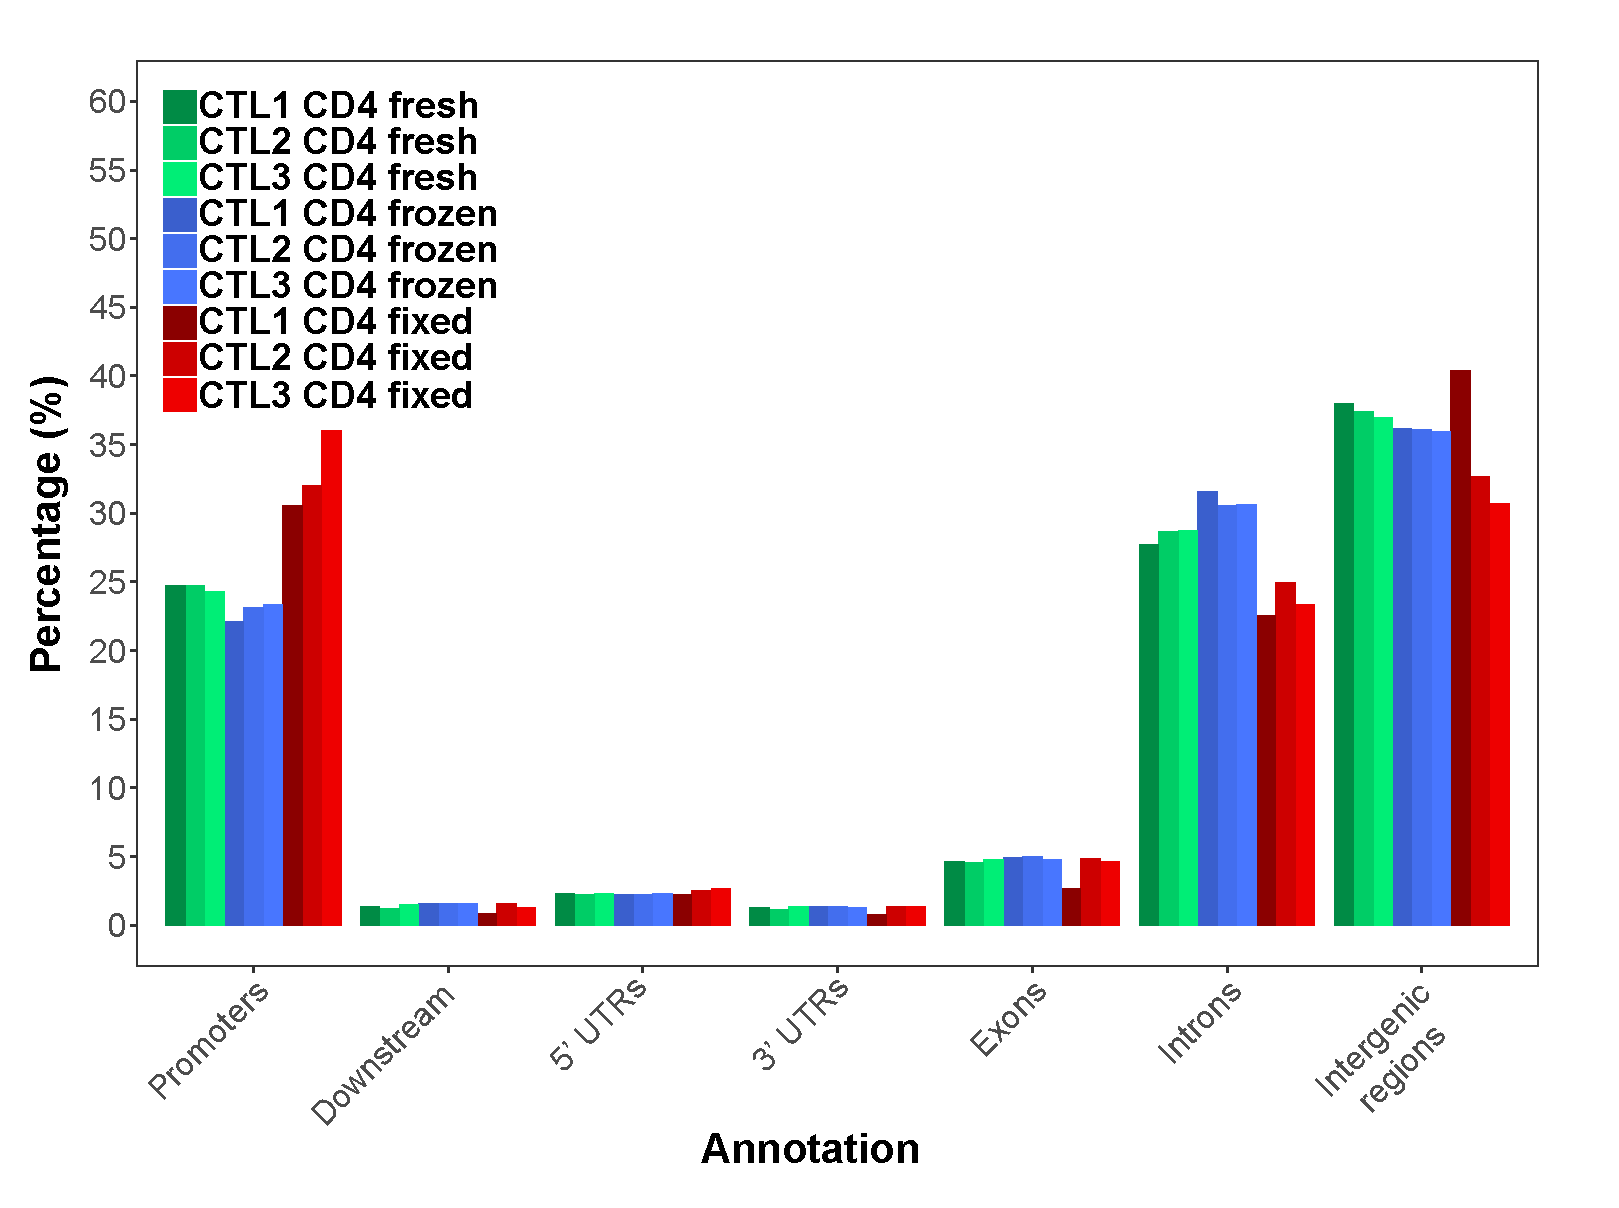
\includegraphics[width=\textwidth]{./Results1/pdfs/Core_ATAC_CD4_fresh_frozen_fixed_general_peak_annotation}
\caption{\textbf{}}
\end{subfigure}
\caption[Genomic features annotation for the ATAC-seq peaks called in each of the fresh,frozen and fixed samples from CD14$^+$ monocytes and total CD4$^+$.]{\textbf{Genomic features annotation for the ATAC-seq peaks called in each of the fresh,frozen and fixed samples from CD14$^+$ monocytes and total CD4$^+$.} Overlap was performed between the genomic features and the list of a) CD14$^+$ monocytes and b) total CD4$^+$ peaks filtered for FDR$<$0.01 in each sample from each of the three conditions (fresh=green, frozen=blue and fixed=red). Annotation for a particular category required a minimum of 1bp overlap.}
\label{fig:Core_ATAC_all_conditions_genomic_features}
\end{figure} 








\subsection{Limitations of ATAC-seq and FAST-ATAC to assess chromatin accessibility in KC}

Due to the fact that KC is one of the most relevant cell types in psoriasis pathophysiology, ATAC-seq as described in Buenrostro \textit{et al.}, 2013 (named as ATAC-seq 1 here) was performed in 50,000 cells of a suspensions isolated from a psoriasis lesional skin biopsy. Two different tranposition times (30 and 40 min) where tested. Since biopsy handling and lesional epidermal KC are particularly challenging this was considered the best system to test the performance of the standard protocol in the clinical setting of interest for the study. Two tranposition times (30 and 40 min) where tested.


\begin{figure}[htbp]
\centering
\begin{subfigure}{0.65\textwidth}
\centering
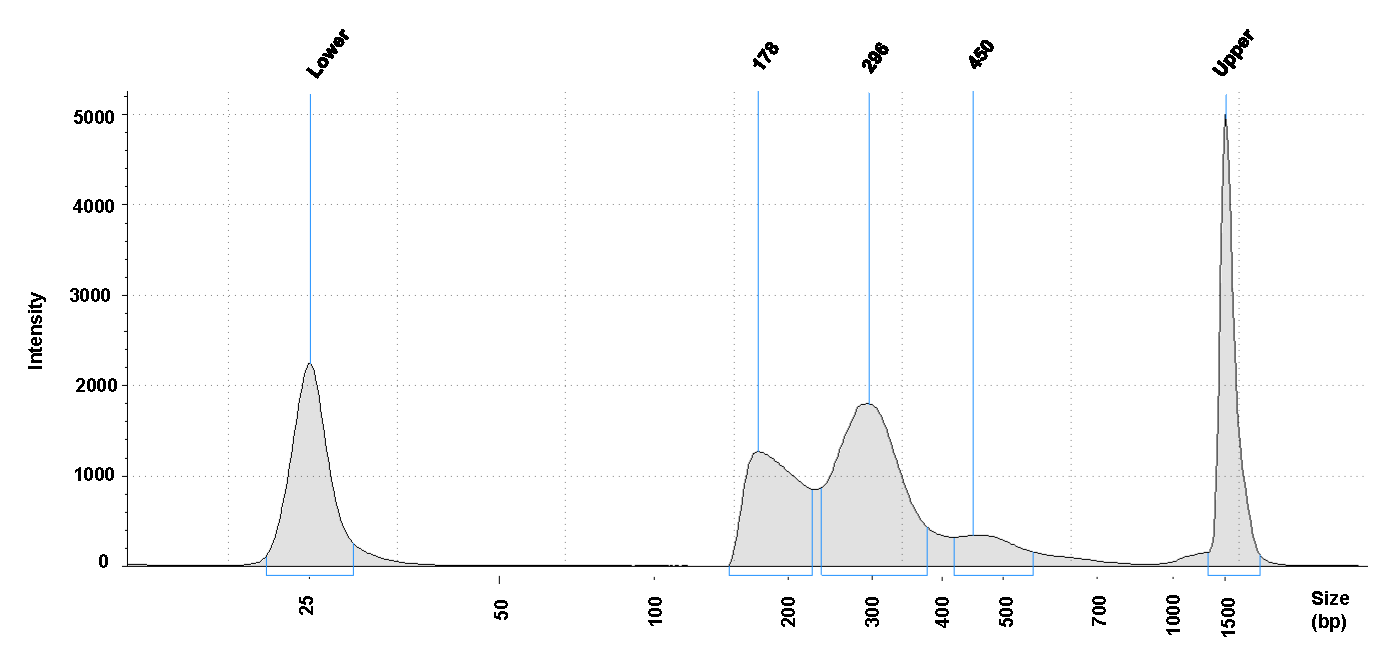
\includegraphics[width=\textwidth]{./Results1/pdfs/ATAC_PS02_tapestation_30min}
\caption{\textbf{}}
\end{subfigure}
\begin{subfigure}{0.45\textwidth}
\centering
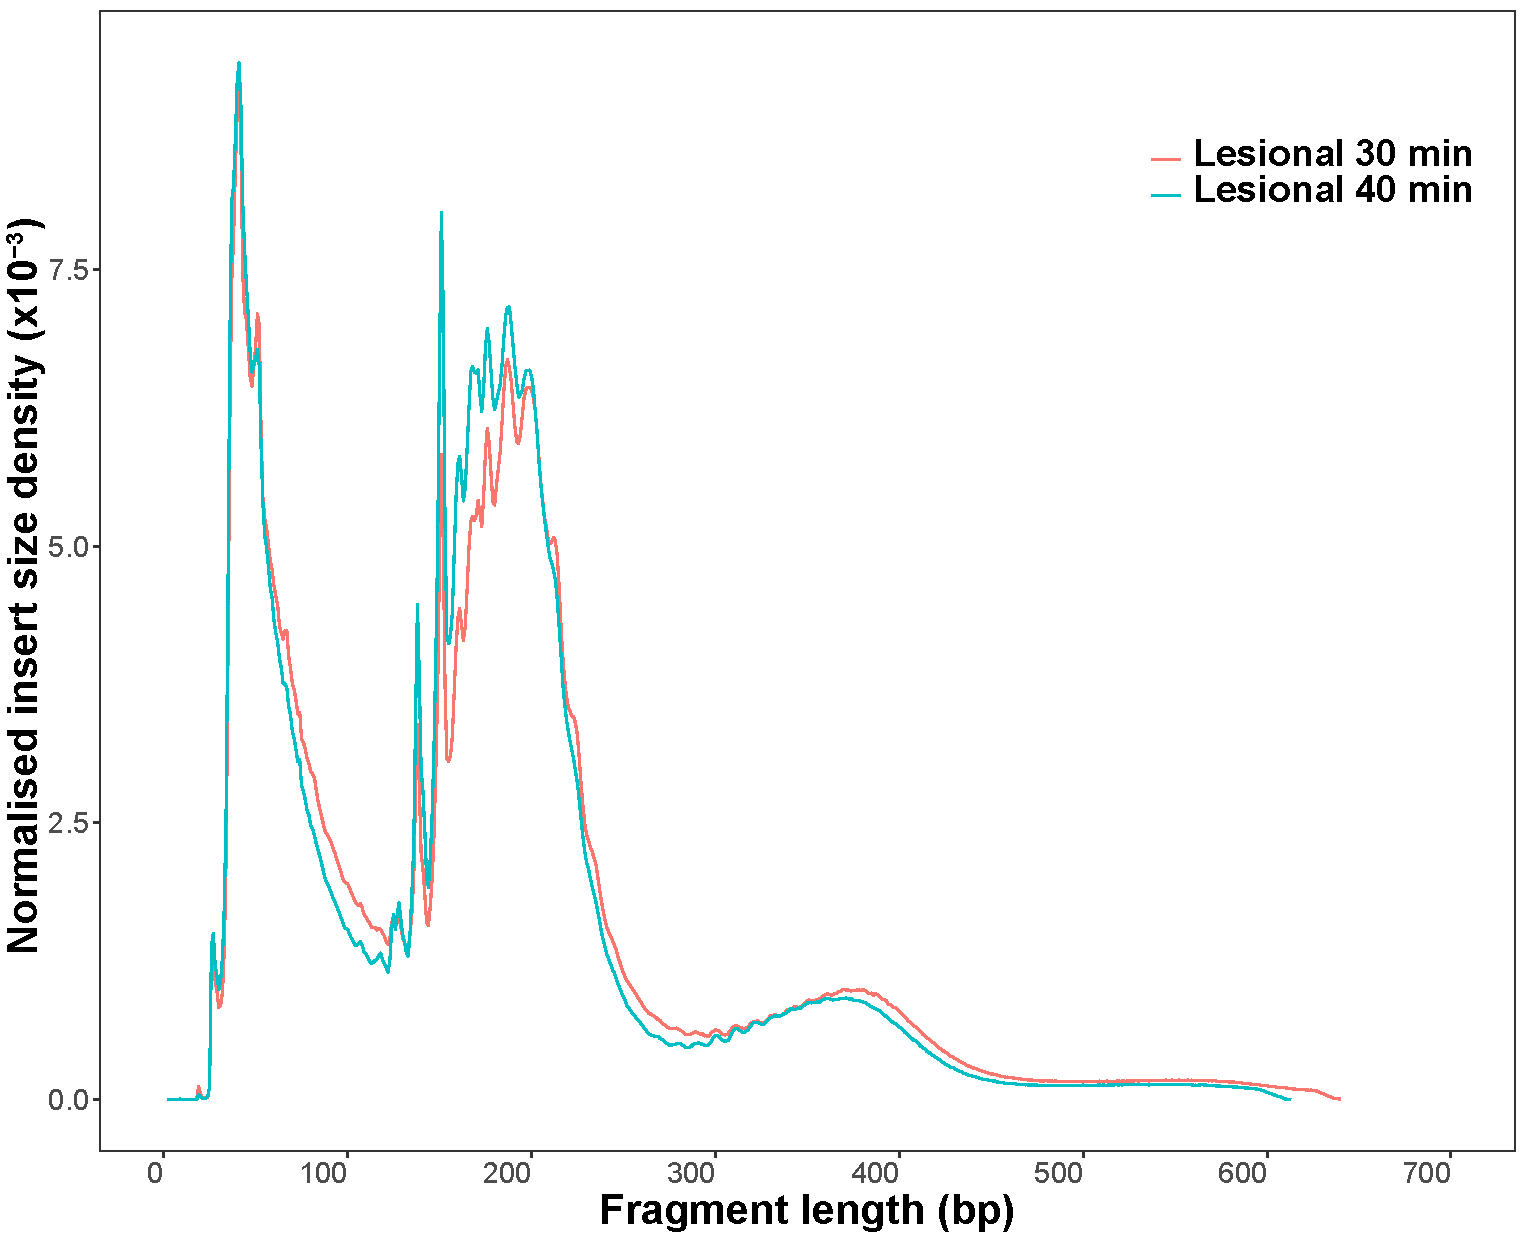
\includegraphics[width=\textwidth]{./Results1/pdfs/ATAC_PS-2_30_40_min_fragment_size_distribution}
\caption{\textbf{}}
\end{subfigure}%
\begin{subfigure}{0.45\textwidth}
\centering
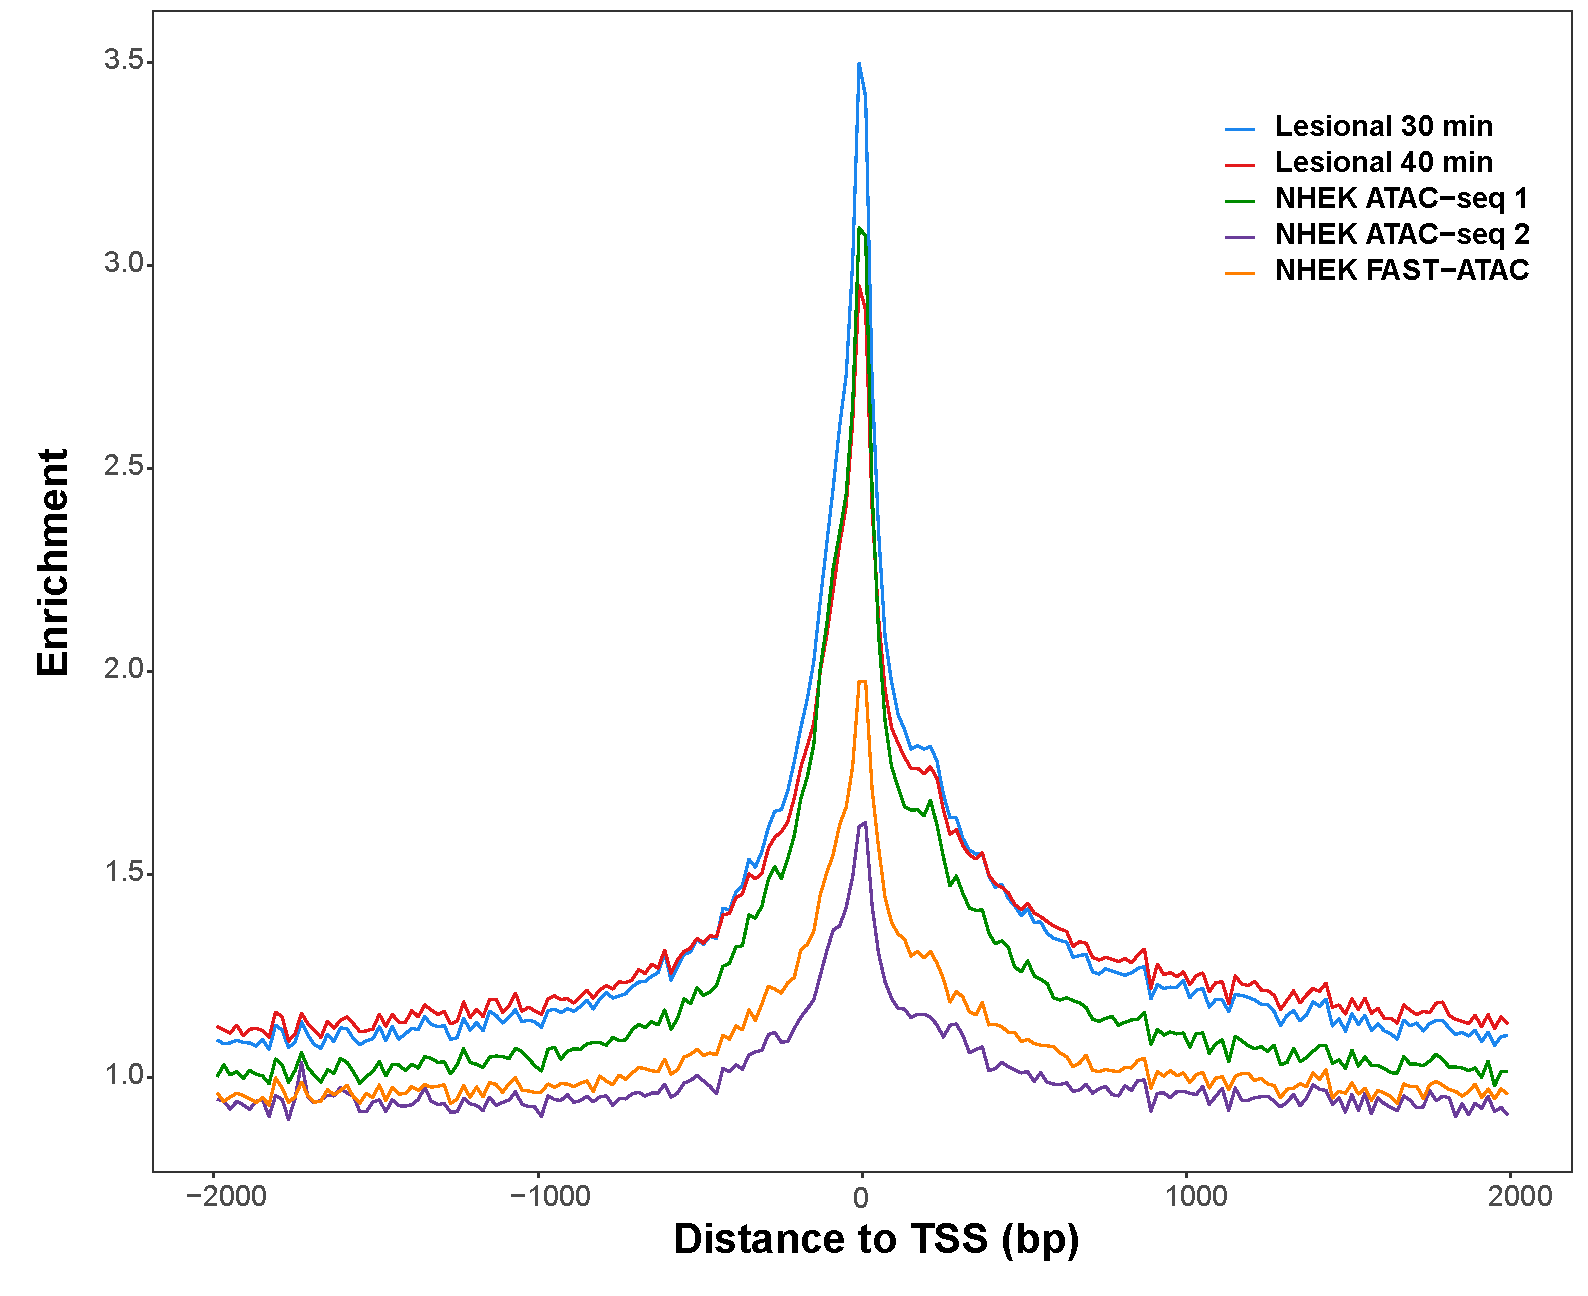
\includegraphics[width=\textwidth]{./Results1/pdfs/ATAC_skin_TSS_enrichment_PS02_30_40min_NHEK_ATAC1_ATAC_2_FAST_ATAC}
\caption{\textbf{}} % to add text to the figure name
\end{subfigure}
\caption[QC assessment of ATAC-seq in KC enriched cell suspension derived from a psoriatic lesional skin biopsy]{\textbf{QC assessment of ATAC-seq in KC enriched cell suspension derived from a psoriatic lesional skin biopsy}. Two transposition times (30 and 40 min) were tested using the standard ATAC-seq protocol (Buenrostro \textit{et al.}, 2013 in 50,000 cells from the same suspension.}
\label{fig:PS02_skin_ATAC_QC_assessment}
\end{figure} 




Although cell suspension obtained from biopsies using trypsinisation of the epidermal sheet are 90\% enriched in KC, they also contain significant amounts of dead cells and free-DNA releases by apoptotic cells. In order to overcome this problem and the impact that it may have over ATAC-seq background signal, viable KC were selected by adherence assay. Biopsy cell suspensions were cultured for 3h in a 96-well plate and washed afterwards to ensure that only the viable and less differentiated KC would remain for down stream analysis. In parallel cultured NHEK were also used to assess the performance of the different ATAC-seq protocols.

Table for the conditions: done
Tapestation profiles of the the chosen condition. done Send the others to supplementary.
QC measurements: for ATAC1, ATAC2 and NHEK, mention frag size distribution done
DHS enrichment for p and q done but not convincing.The complex network of keratin filaments in stratified epithelia is tightly regulated during squamous cell differentiation. Keratin 14 (K14) is expressed in mitotically active basal layer cells, along with its partner keratin 5(K5), and their expression is down-regulated as cells differentiate.


\begin{table}[htbp]
%\setlength{\tabcolsep}{20pt}
%\renewcommand{\arraystretch}{1.5}
\begin{tabular}{@{} c c c}
\toprule
\textbf{Protocol} & \textbf{Lysis and} & \textbf{Key parameters} \\
                  & \textbf{transposition} &  \\
\midrule
\midrule
Buenrostro \texit{et al.,} 2013 & Two steps & 0.1\% NP-40 and 2.5$\micro$L Tn5  \\
&&&
Bao \texit{et al.,} 2015        &Two steps   & 0.05\% NP-40 and 5$\micro$L Tn5  \\
&&&
                                &          & C1: 0.01\% digitonin, 0.5$\micro$L Tn5 \\
                                &          & C2: 0.01\% digitonin, 2.5$\micro$L Tn5 \\
 Corces \texit{et al.,} 2016    & One step & C3: 0.025\% digitonin, 0.5$\micro$L Tn5 \\
													      &          & C4: 0.025\% digitonin, 2.5 $\micro$L Tn5 \\
\bottomrule
\end{tabular}
\medskip %gap
\caption[Description of the most relevant parameter from the ATAC-seq and FAST-ATAC protocols assayed in NHEK and skin biopsies.]{\textbf{ Description of the most relevant parameter from the ATAC-seq and FAST-ATAC protocols assayed in NHEK and skin biopsies.}Transposition for all the different protocols was 30 min.}
\label{tab:ATAC_skin_optimisation_protocols}
\end{table}
\bigskip %bigger space



\begin{figure}[htbp]
\centering
\begin{subfigure}{0.48\textwidth}
\centering
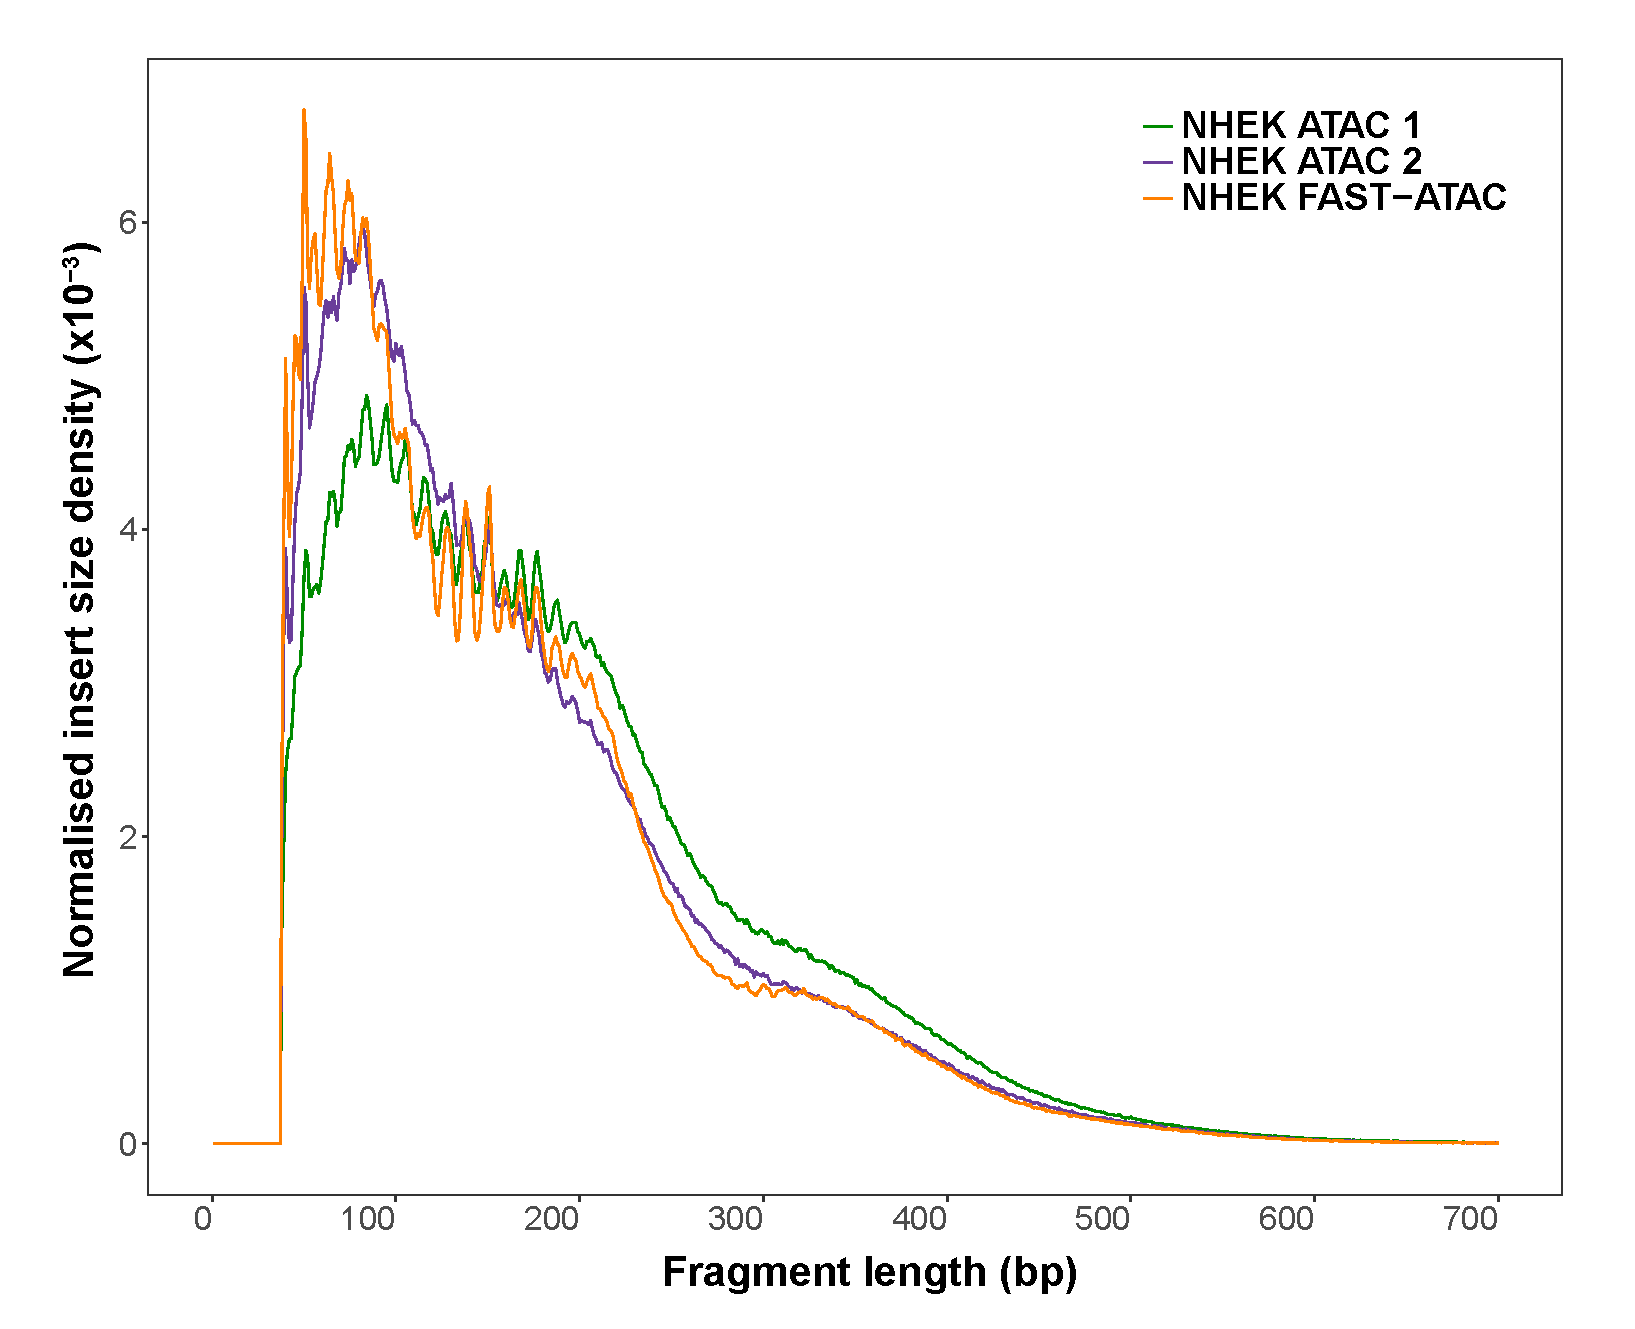
\includegraphics[width=\textwidth]{./Results1/pdfs/ATAC_NHEK_ATAC1_ATAC2_FAST_ATAC_fragment_size_distribution}
\caption{\textbf{}}
\end{subfigure}%
\begin{subfigure}{0.48\textwidth}
\centering
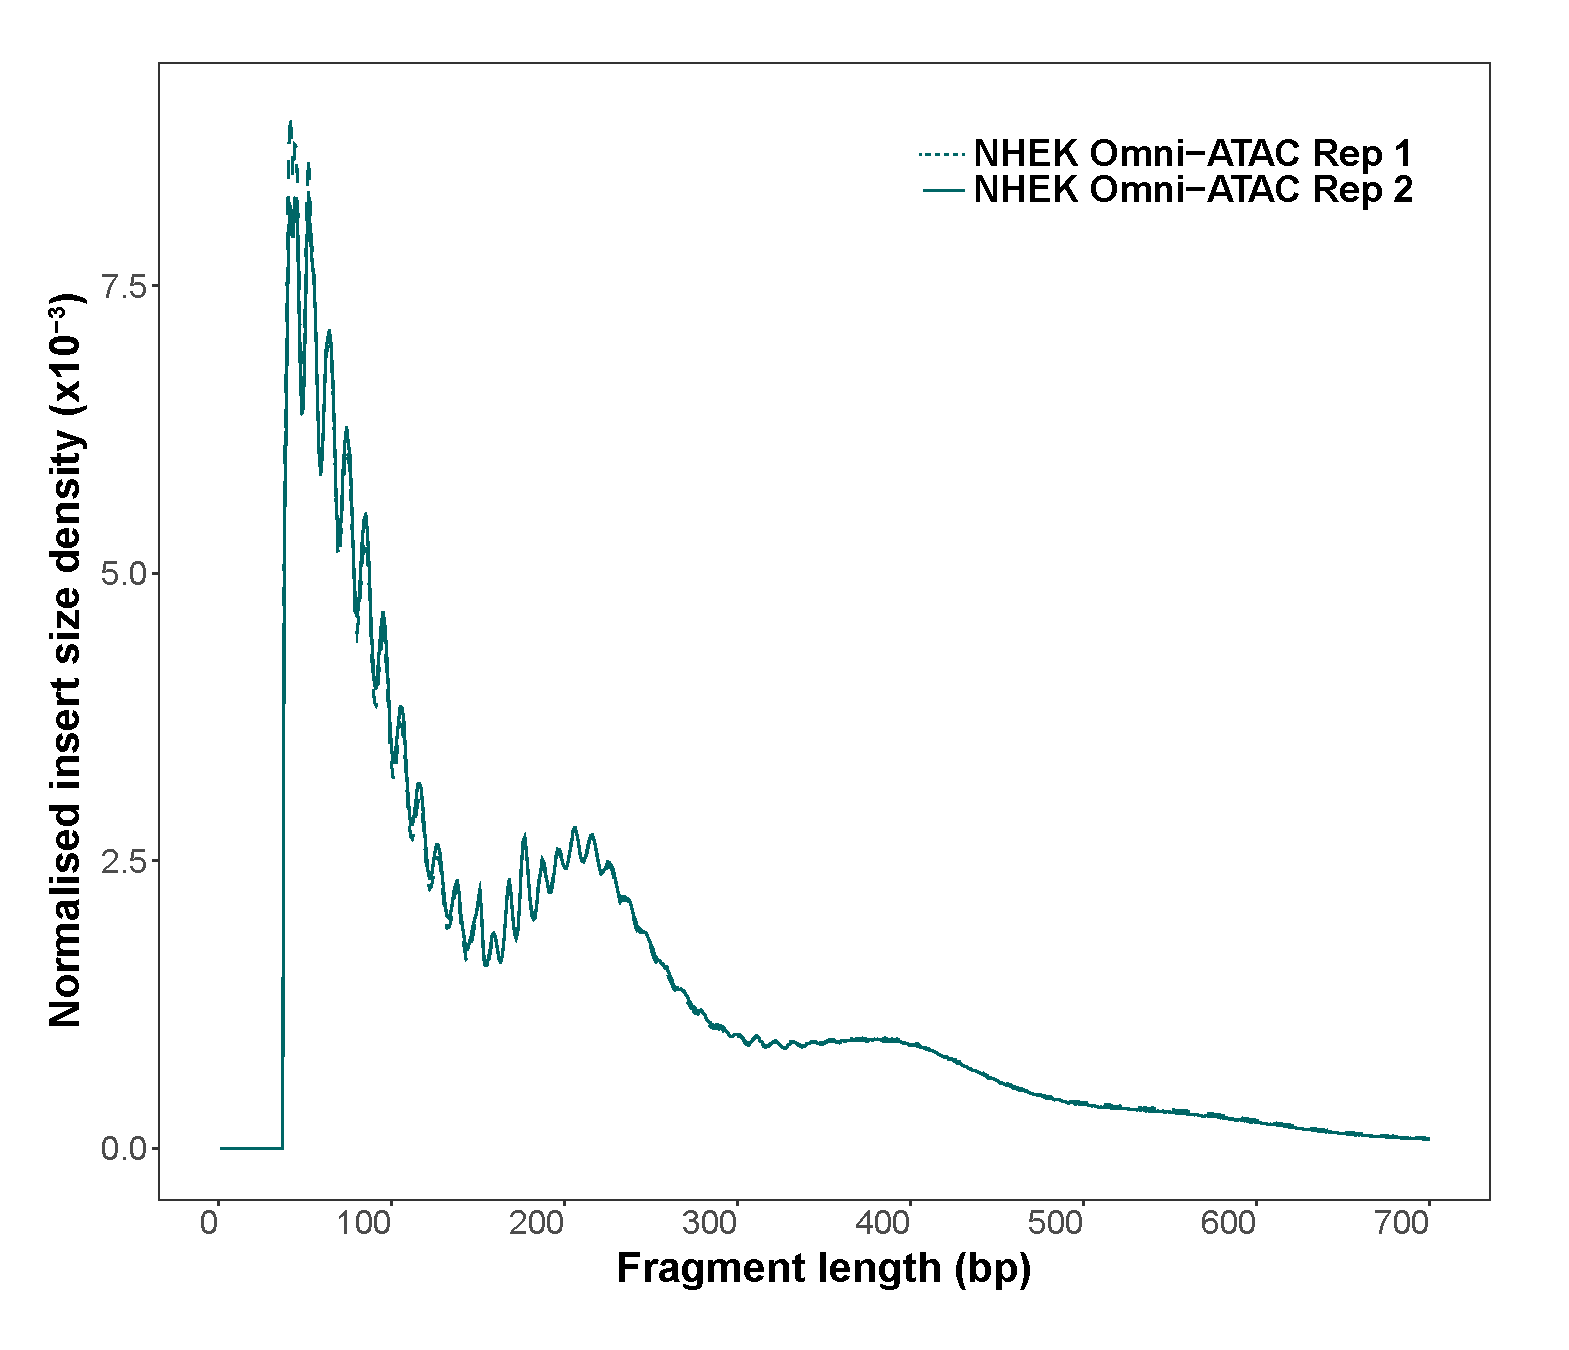
\includegraphics[width=\textwidth]{./Results1/pdfs/ATAC_NHEK_Omni_ATAC_fragment_size_distribution}
\caption{\textbf{}}
\end{subfigure}
\begin{subfigure}{0.5\textwidth}
\centering
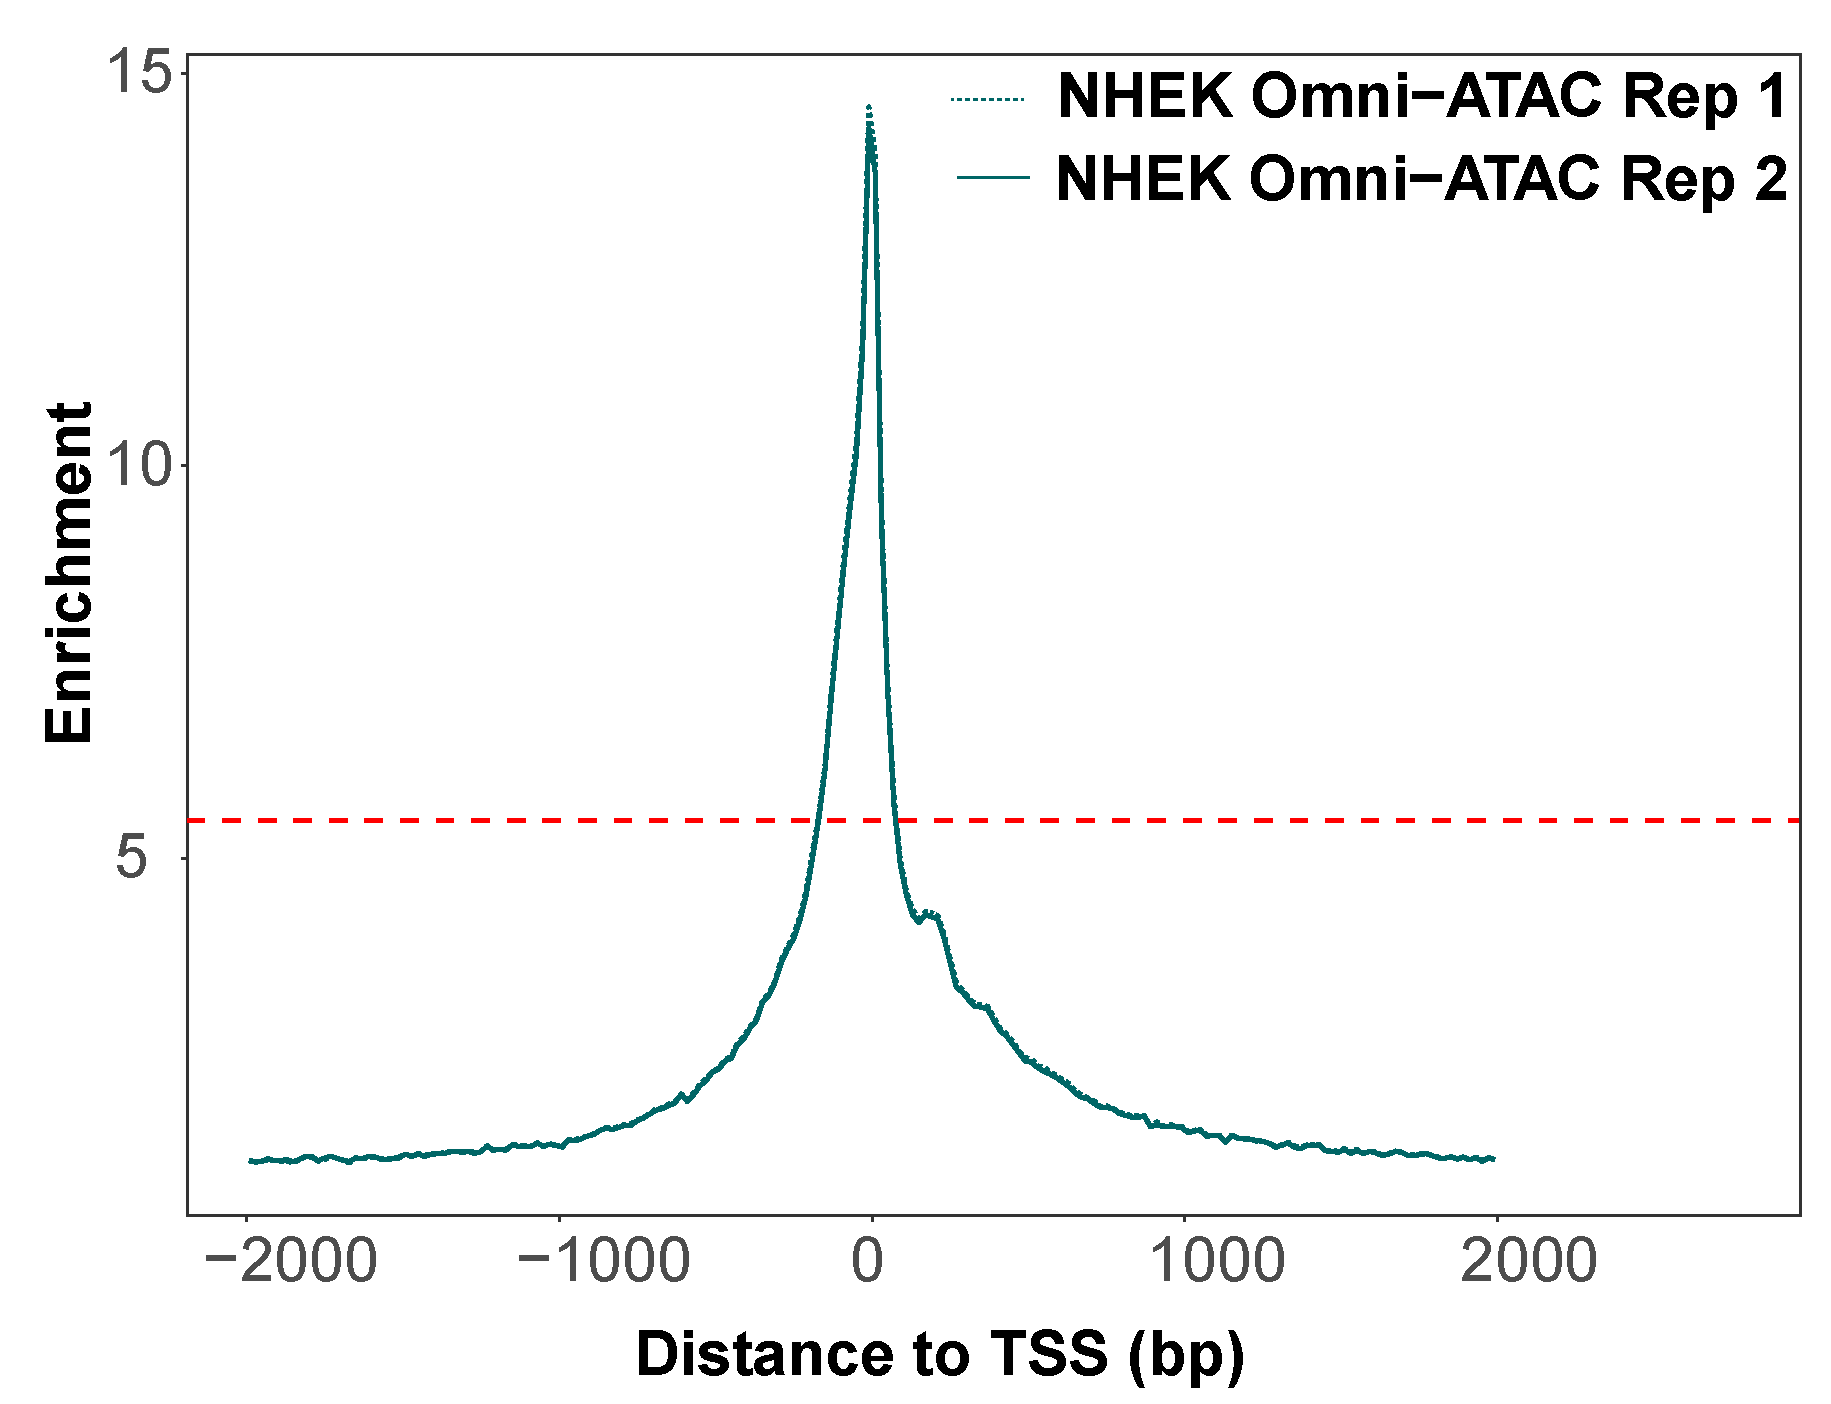
\includegraphics[width=\textwidth]{./Results1/pdfs/ATAC_skin_TSS_enrichment_NHEK_omni_ATAC}
\caption{\textbf{}} % to add text to the figure name
\end{subfigure}%
\caption[QC assessment of FAST-ATAC and Omni-ATAC in cultured NHEK]{\textbf{QC assessment of FAST-ATAC and Omni-ATAC in cultured NHEK.\\
}}
\label{fig:PS02_skin_ATAC_QC_assessment}
\end{figure} 






Omni-ATAC
Tapestation profiles of the the chosen condition include it with the supplementary that includes all other tapestation profiles.done
QC measurements: frag size distribution and TSS done
Track including all skin samples

Think of what to include about the biopsies in supplementary done



\begin{figure}[htbp]
\centering
\begin{subfigure}{0.5\textwidth}
\centering
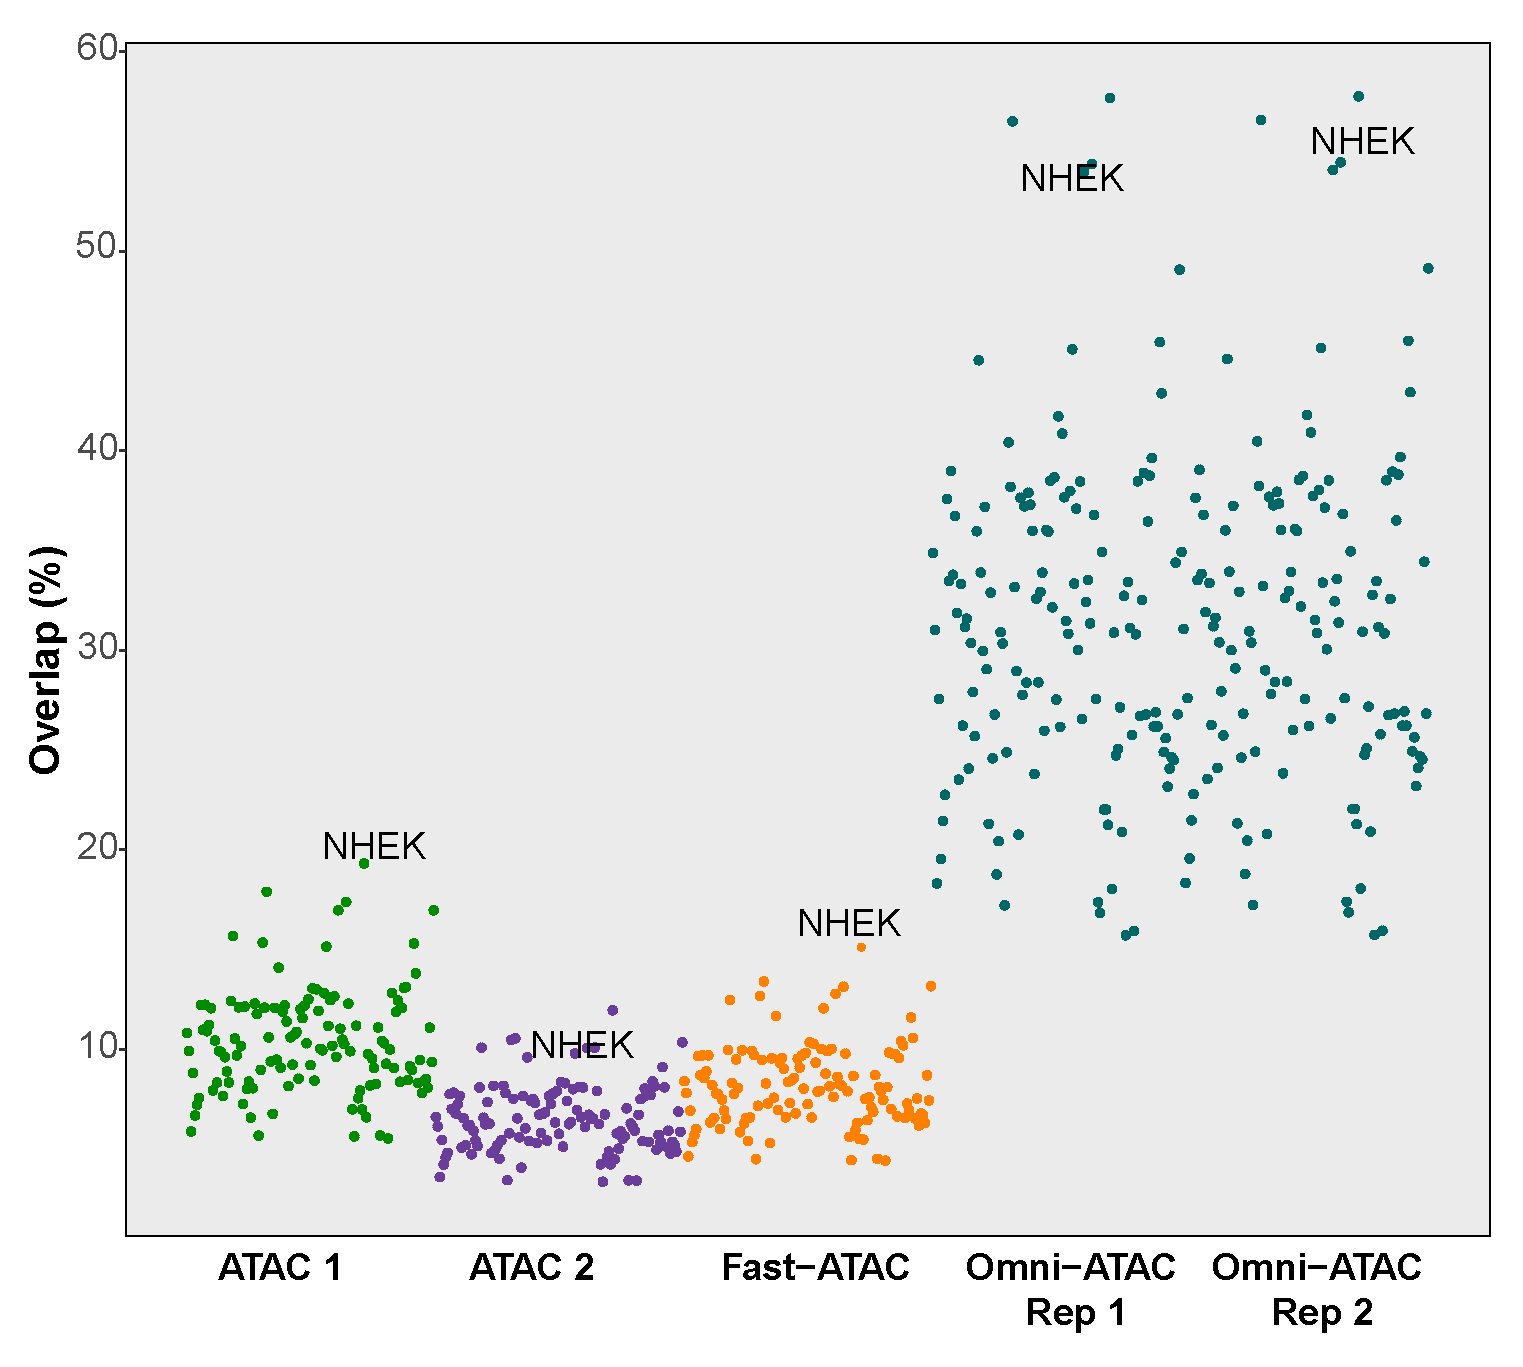
\includegraphics[width=\textwidth]{./Results1/pdfs/ENCODE_125_cell_types_overlap_FAST_ATAC_Omni_ATAC_pval_2}
\caption{\textbf{}}
% The percentage sign indicated that the other subfig goes side by side
\end{subfigure}%
\begin{subfigure}{0.5\textwidth}
\centering
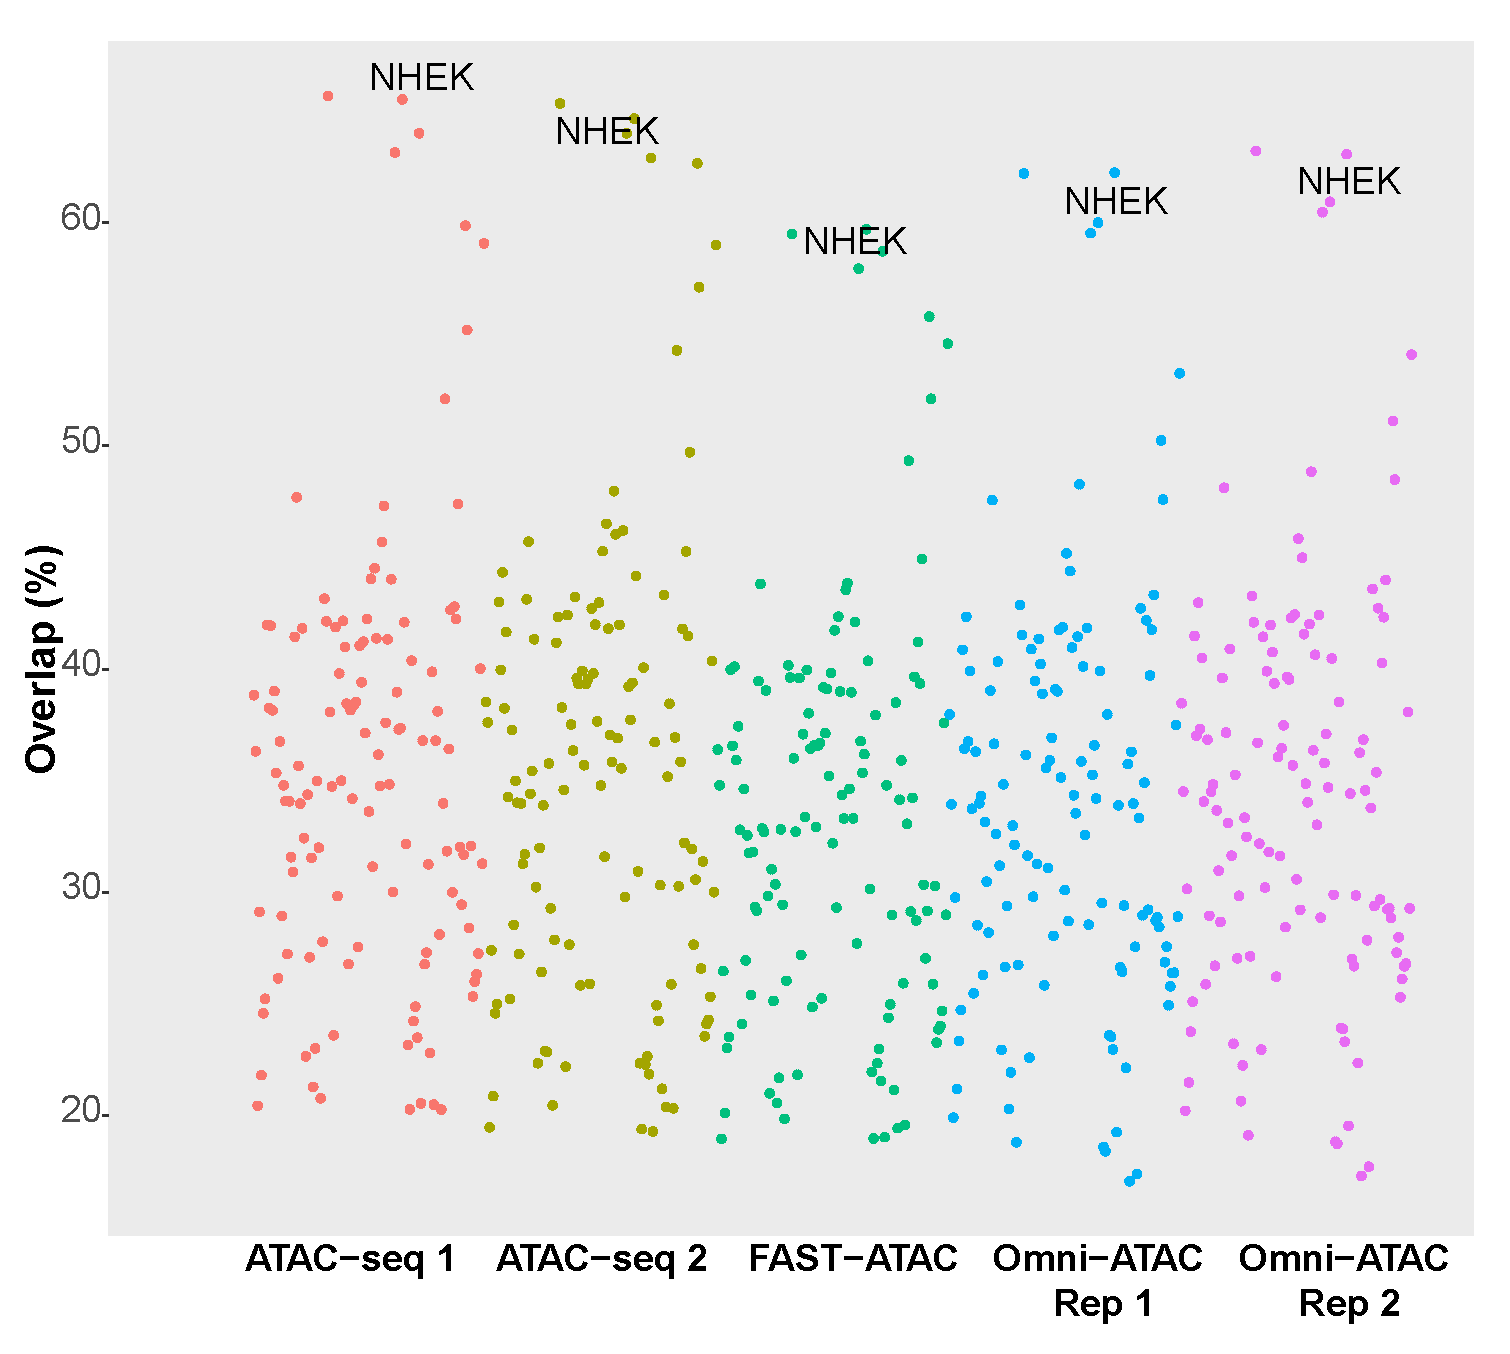
\includegraphics[width=\textwidth]{./Results1/pdfs/ENCODE_125_cell_types_overlap_FAST_ATAC_Omni_ATAC_qval_2}
\caption{\textbf{}}
\end{subfigure}
\begin{subfigure}{0.5\textwidth}
\centering
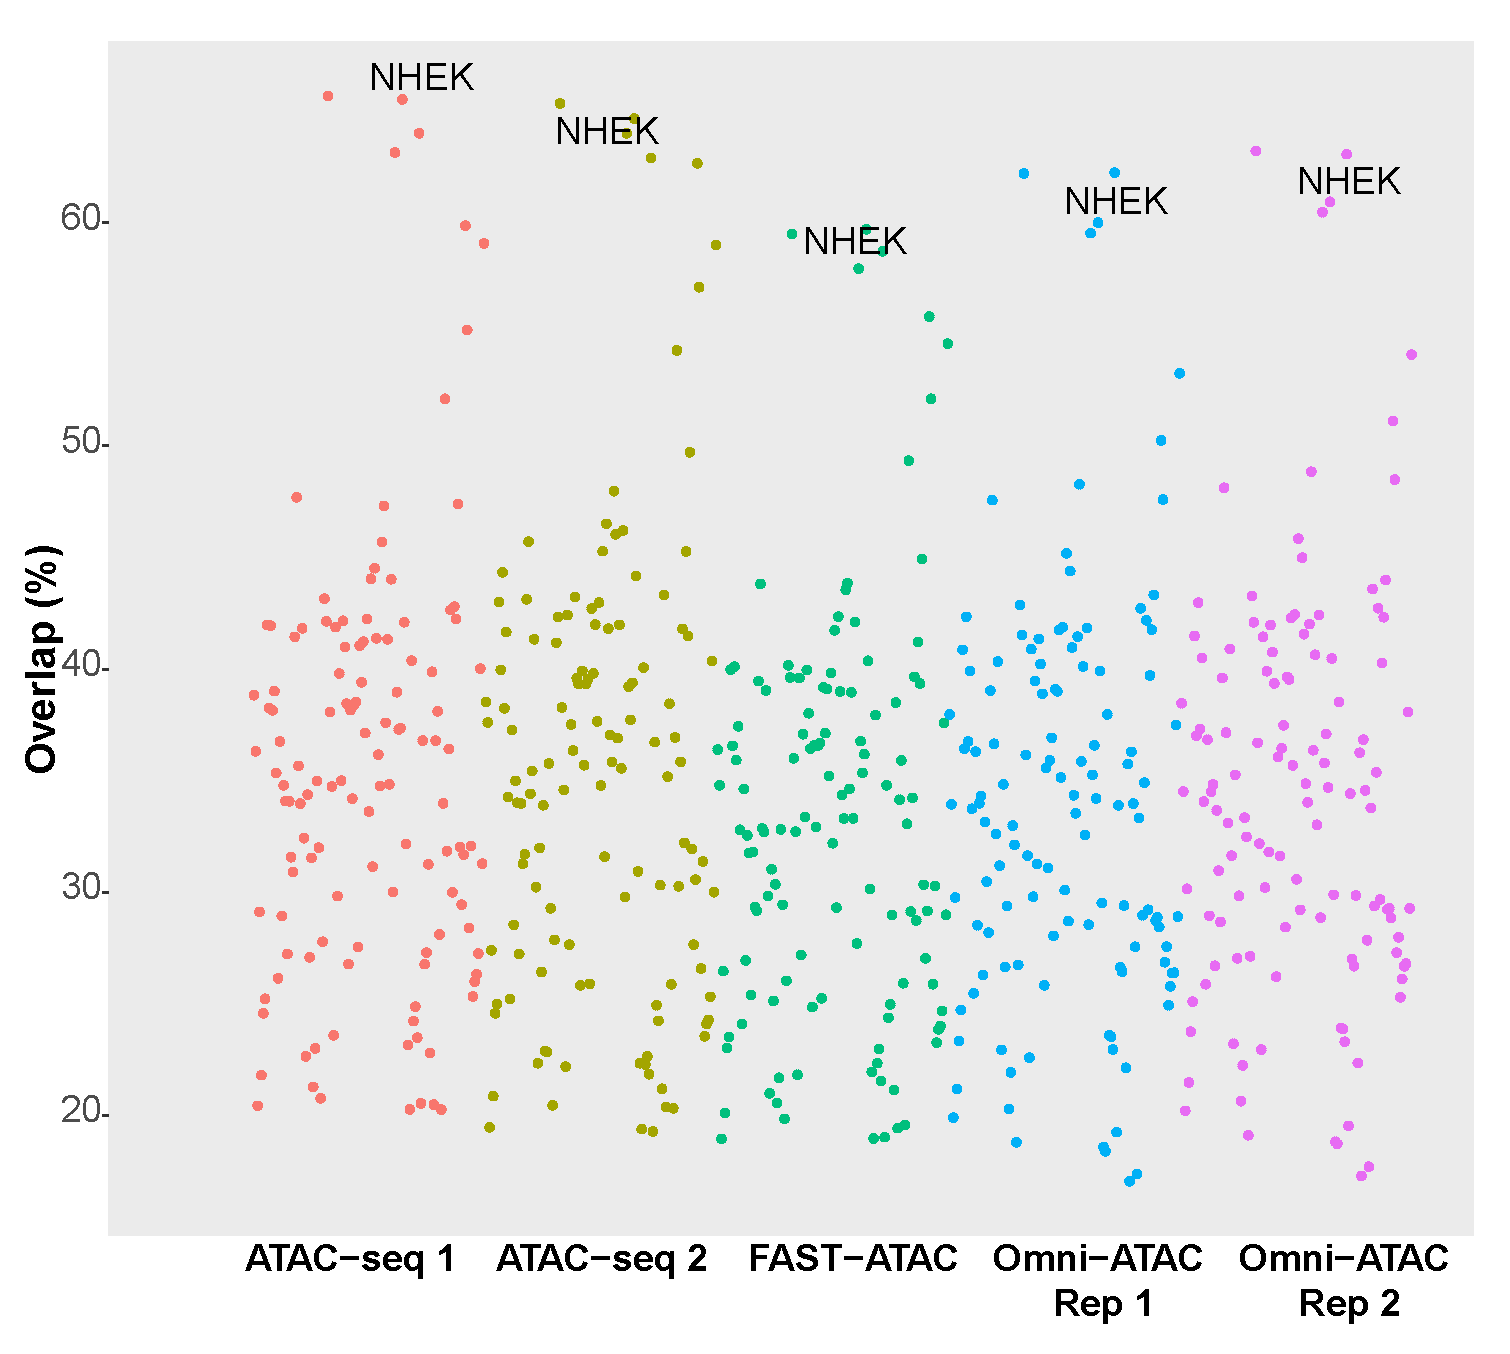
\includegraphics[width=\textwidth]{./Results1/pdfs/ENCODE_125_cell_types_overlap_FAST_ATAC_Omni_ATAC_qval_2}
\caption{\textbf{}} % to add text to the figure name
\end{subfigure}%
\caption[QC assessment of Omni-ATAC in NHEK and chromatin accessibility signal for the samples generated with the different ATAC-seq protocols]{\textbf{QC assessment of Omni-ATAC in NHEK and chromatin accessibility signal for the samples generated with the different ATAC-seq protocols}.\\}
\label{fig:Omni_ATAC_NHEK_QC_assessment_and_all_tracks}
\end{figure} 



\subsection{Discussion}
Maybe justify in the dicussion the use of DESEq2 and limma shared based on Alasoo observation of noise effect in limma